\chapter[Интегративное моделирование амилоидоподобных фибрилл]{Интегративное моделирование амилоидоподобных фибрилл\footnote{При подготовке данного раздела диссертации использованы следующие публикации, выполненные автором лично или в соавторстве, в которых, согласно Положению о присуждении ученых степеней в МГУ, отражены основные результаты, положения и выводы исследования: \cite{shaytan_self-assembling_2011,shaytan_self-organizing_2011,yolamanova_peptide_2013}.}}  \label{part4_amyloid}


В данной главе излагаются подходы, разработанные автором для интегративного моделирования структуры амилоидоподобных фибрилл. Особенностью подходов является использование экспериментальных данных как на этапе конструирования возможных межмолекулярных укладок пептидов в фибриллах, так и на этапе оценки крупномасштабной морфологии фибрилл. Излагаются работы по изучению фибрилл из олигомеров проводящего полимера тиофена и пептидов, а также конструированию положительно заряженных амилоидоподобных фибрилл, ускоряющих вирусную трансдукцию.
Материалы данной главы включают данные из диссертации автора на соискание степени Dr. Rer. Nat. \cite{shaytan_thesis_ulm_2012} и следующих статьей \cite{shaytan_self-assembling_2011,shaytan_self-organizing_2011,yolamanova_peptide_2013}. 


\section{Амилоиды и материалы на основе амилоидов}

    В настоящем разделе мы рассмотрим феномен амилоидных фибрилл, обсудим их структуру, свойства самосборки и экспериментальные методы, используемые для их исследования. Также дадим обзор достижений в разработке новых материалов, основанных на ковалентном присоединении синтетических фрагментов к образующим $\beta$-лист (амилоидогенным) пептидам. Упор будет сделан на экспериментальных результатах для PEO-функционализированных алкилированных  диблок олигомеров кватротиофен-пептид, которые являются основным объектом следующего раздела.

\subsection{Строение природных амилоидных фибрилл и их полиморфизм}

    Термин ``амилоидные фибриллы'' в его современном понимании относится к удлиненным белковым агрегатам, характеризующимся своей длинной и относительно прямой морфологией, характерными картинами дифракции \cite{sunde_common_1997}, специфическими свойствами связывания некоторых красителей и жесткой структурой ядра \cite{kumar_mechanisms_2010}. На сегодняшний день идентифицировано более 20 белков плазмы, которые могут образовывать патологические отложения амилоидного характера в организме человека, что связано со многими разрушительными заболеваниями, такими как болезнь Альцгеймера, болезнь Паркинсона, диабет II типа, болезнь Хантингтона, болезнь Крейтцфельдта-Якоба, прионные расстройства и многими другими \cite{chiti_protein_2006,makin_structures_2005,rochet_amyloid_2000}. Известно, что патологическое образование амилоидных фибрилл включает структурную перестройку нативного состояния белков в конформацию фибрилл, богатую $\beta$-слоями \cite{sipe_beta-pleated_2008}. Недавно выяснилось, что практически все белки потенциально могут собираться в амилоидные фибриллы \cite{chiti_protein_2006,chiti_designing_1999} и были получены многие модельные последовательности de novo, которые агрегируют в фибриллы при определенных условиях \cite{janek_water-soluble_1999}.

    Амилоидные фибриллы имеют диаметр примерно 7-10 нм (по данным электронной микроскопии (ЭМ) или атомно-силовой микроскопии (АСМ) \cite{chiti_protein_2006,makin_structures_2005,rochet_amyloid_2000}) и обычно состоят из 2-6 протофиламентов. Внутренняя структура всех амилоидных фибрилл имеет один и тот же структурный мотив, перекрестный $\beta$-мотив, который выявляется характерной картиной дифракции рентгеновских лучей \cite{sunde_common_1997} с меридиональными рефлексами соответсвующими 4,7–4,9 \AA{} (так называемое расстояние между основными цепями) и более диффузными экваториальными рефлексами соответсвующими приблизительно 10\AA{} (наблюдались вариации от 8,8 до 14,6\AA{} \cite{fandrich_behaviour_2002}) (так называемый интервал боковых цепей), эти рефлексы свидетельствуют о высоком порядке и периодичности внутренней структуры фибрилл вдоль и перпендикулярно направлению фибрилл. Понимание молекулярных деталей самосборки пептидов в фибриллярные агрегаты было сложной задачей из-за большого размера, низкой растворимости и некристаллической и гетерогенной природы фибрилл. В течение последнего десятилетия значительный прогресс в нашем понимании принципов образования фибрилл был достигнут благодаря многочисленным экспериментальным и теоретическим исследованиям и, что важно, разрешению расположения пептидов на атомистическом уровне с помощью рентгеновской кристаллографии и твердотельного ЯМР. Для получения дополнительной информации можно рекомендовать ряд недавних обзоров по структуре и образованию амилоидных (-подобных) фибрилл \cite{kumar_mechanisms_2010,rambaran_amyloid_2008,fandrich_structural_2009}. Понимание структуры амилоидных фибрилл значительно улучшилось с помощью рентгеноструктурных исследований микрокристаллов амилоид-образующих сегментов амилоидогенных белков \cite{nelson_structure_2005,sawaya_atomic_2007}. Эти исследования показывают, что перекрестные $\beta$-мотивы в амилоидных фибриллах, образованные этими амилоидогенными сегментами, состоят из пары $\beta$-листов (рис. \ref{fig:p4_p1_f2}), состоящих из выровненных пептидных фрагментов. Два таких $\beta$-листа дополняют друг друга, образуя пару листовых структур, в которых боковые цепи, выступающие из двух листов, интеркалируют, образуя сухую ``стерическую молнию'' (рис. \ref{fig:p4_p1_f2}б), которая считается важным стабилизирующим взаимодействием.
  
    Исследования методами твердотельного ЯМР в сочетании с измерениями по изображениям электронной микроскопии позволили предложить прямые атомистические модели расположения молекул в скрученных протофиламентах амилоида-$\beta_{1-40}$ \cite{petkova_experimental_2006,tycko_molecular_2006} (рис. \ref{fig:p4_p1_f2}в). Две $\beta$-цепи каждой молекулы амилоид-$\beta_{1-40}$ соединены через изгибную область, содержащую остатки 25–29, и являются частями двух разных совпадающих параллельных $\beta$-листов, взаимодействующих через свои боковые цепи в одном протофиламенте. Одиночный протофиламент амилоид-$\beta_{1-40}$, по-видимому, включает два перекрестных $\beta$-мотива, то есть четыре $\beta$-листа с расстоянием между листами $\sim$1 нм. Протофиламент проявляет левостороннюю спиральную закрутку, что характерно для $\beta$-листов.

\begin{figure} [H]
    \centering
    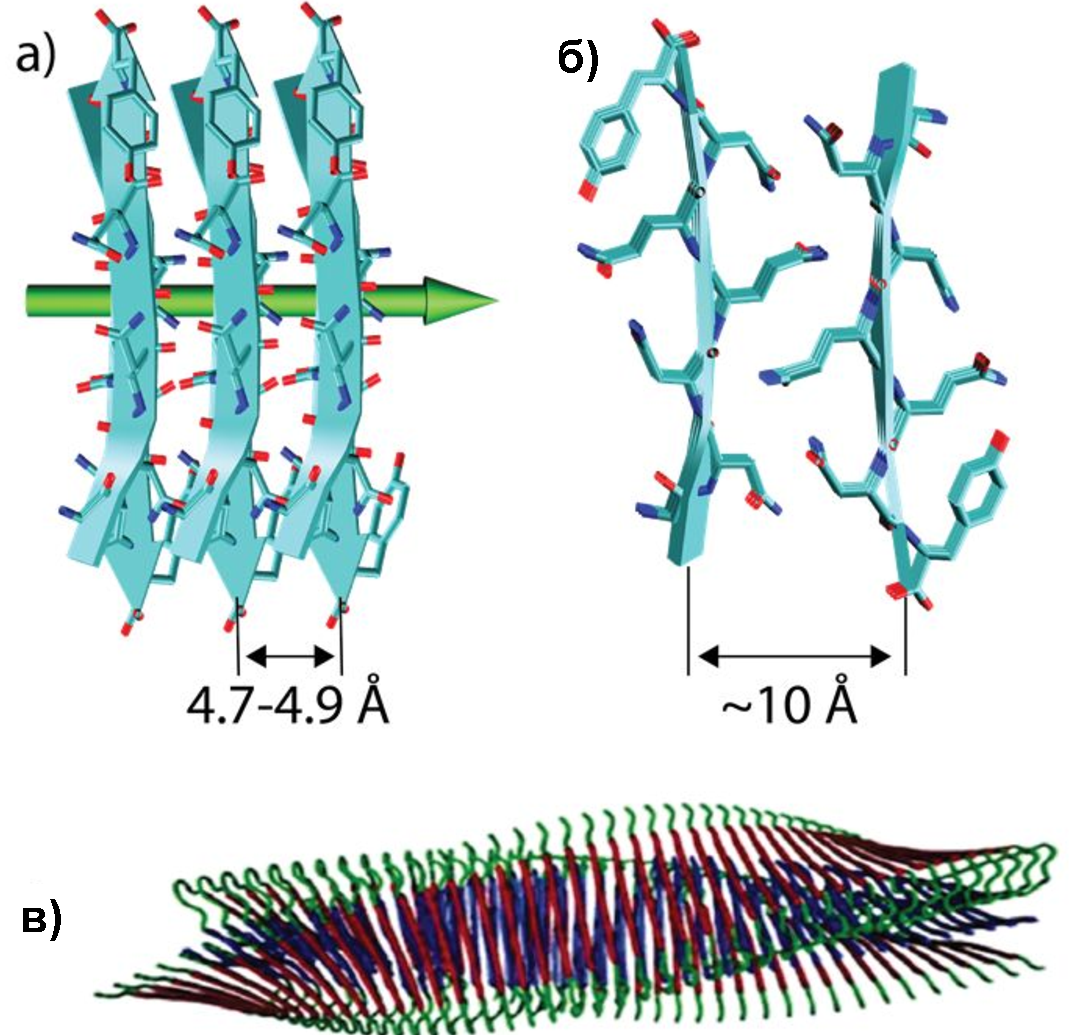
\includegraphics[width=\textwidth]{images/p4/punkt1/part4_p1_f2.pdf}
    \caption[Модели расположения $\beta$-тяжей в амилоидных протофибриллах]{Модели расположения $\beta$-тяжей в амилоидных протофибриллах посредством поперечной $\beta$-структуры. Вид сбоку (а) и вид сверху (б) перекрестной $\beta$-структуры ядра фибриллы на примере микрокристаллов пептидных фрагментов дрожжевого белка Sup35 \cite{nelson_structure_2005}, показано расстояние между основной и боковой цепями. Зеленая стрелка показывает направление фибрилл. На панели (б) видна стерическая застежка-молния между боковыми цепями соседних листов. (в) Ленточная диаграмма протофиламента амилоид-$\beta_{1-40}$, если смотреть параллельно оси фибриллы. Структурная модель основана на данных твердотельного ЯМР в сочетании с ограничениями из данных электронной микроскопии. Каждая молекула A$\beta$ вносит две $\beta$-цепи в параллельные $\beta$-листы. Основано на материалах статьи \cite{petkova_experimental_2006}}
    \label{fig:p4_p1_f2}
\end{figure}
  
    Вышеупомянутые примеры, однако, далеко не единственные возможные молекулярные структуры, согласующиеся с перекрестным $\beta$-мотивом. Внутренняя структура последних может существенно различаться в разных фибриллах. Рентгеновские структуры 13 микрокристаллов ряда амилоидобразующих сегментов амилоидогенных белков, решенные Sawaya et al. \cite{sawaya_atomic_2007} пролили дополнительный свет на то, как перекрестный $\beta$ мотив может проявлять вариации. В зависимости от ориентации $\beta$-нитей (параллельных или антипараллельных) внутри листов, от ориентации $\beta$-листов (параллельных или антипараллельных) относительно друг друга или от упаковки листов (лицом к лицу или лицом к спине) 8 различных основных классов расположения ``стерических застежек-молний'' могут в принципе согласовываться с перекрестный $\beta$ мотивом (см. рис. \ref{fig:p4_p1_f3}), 5 из которых уже наблюдались в решенных атомистических структурах микрокристаллов. Твердотельный ЯМР амилоидных фибрилл, образованных различными пептидами, гомологичными участкам пептида Альцгеймера, также показал, что $\beta$-лист может располагаться по-разному - параллельно или антипараллельно внутри протофиламентов в зависимости от свойств полипептида-предшественника \cite{gordon_increasing_2004,balbach_supramolecular_2002,petkova_solid_2004,petkova_self-propagating_2005}, хотя, как описано ранее, исследования фибрилл, образованных из полноразмерного амилоида-$\beta$, показали, что пептид сворачивается в $\beta$-изгибную структуру, которая затем связывается с другими молекулами, образуя параллельную $\beta$-структуру \cite{petkova_experimental_2006,luhrs_3d_2005}.

\begin{figure} [H]
    \centering
    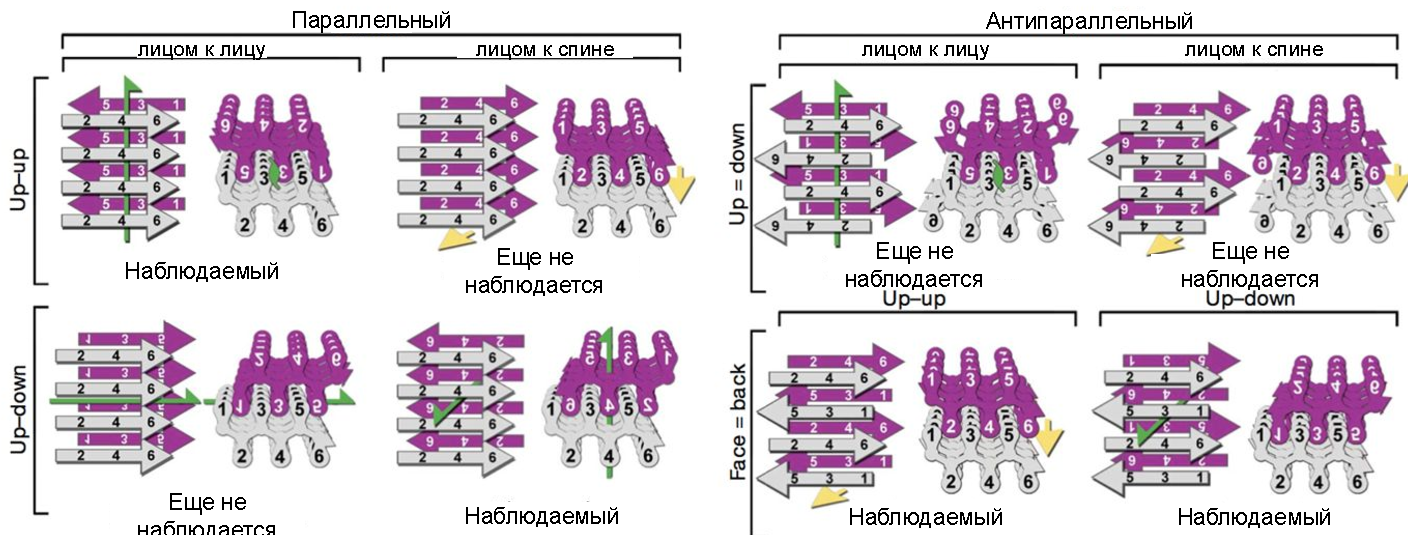
\includegraphics[width=\textwidth]{images/p4/punkt1/part4_p1_f3.pdf}
    \caption[Возможные варианты расположения $\beta$-листов в перекрестном $\beta$-мотиве]{Возможные варианты расположения $\beta$-листов в перекрестном $\beta$-мотиве. Два идентичных листа можно классифицировать по: ориентации их граней (либо ``лицом к лицу'', либо ``лицом к спине''), ориентации их нитей (при этом оба листа имеют одинаковый край нити ``вверх'', или один ``вверх'', а другой ``вниз''), а также от того, параллельны ли нити в листах или антипараллельны. Оба вида сбоку (слева) и виды сверху (справа) показывают, какой из шести остатков сегмента образует застежку-молнию, а какой - смотрит наружу. Зеленые стрелки показывают винтовые оси симметрии второго порядка, а желтые стрелки показывают трансляционную симметрию. Под каждым классом перечислены белковые сегменты, принадлежащие этому классу. По материалам Sawaya et al. \cite{sawaya_atomic_2007}.}
    \label{fig:p4_p1_f3}
\end{figure}

    Хотя за последние десятилетия был достигнут значительный прогресс, мы все еще далеки от того, чтобы сказать, что полная картина самосборки фибрилл теперь понятна как на молекулярном, так и на нано- и микромасштабах. Оказывается, амилоидные (-подобные) фибриллы имеют тенденцию быть высокополиморфными структурами \cite{fandrich_structural_2009} со сложным взаимодействием на молекулярном уровне, которые могут приводить к широкому спектру различных агрегатов с различной морфологией. Структурный и морфологический полиморфизм амилоидных фибрилл простирается намного дальше, чем просто зависимые от последовательности вариации структуры перекрестного $\beta$-мотива - одни и те же полипептидные последовательности, как известно, образуют фибриллы различной морфологии в зависимости от таких факторов, как значение pH, температуры, наличие перемешивания, солей и других сорастворенных веществ \cite{petkova_self-propagating_2005,pedersen_changing_2006,toyama_structural_2007,makarava_same_2008,verel_polymorphism_2008,klement_effect_2007}. Даже в одних и тех же условиях и в одном образце могут существовать значительные вариации морфологии фибрилл. Различное расположение протофиламентов может приводить к различным морфологиям амилоидных фибрилл. Эти фибриллы могут различаться по нескольким структурным свойствам, таким как толщина поперечного сечения фибриллы, шаг спирали, способ слипания и переплетения амилоидных протофиламентов с образованием трехмерной структуры фибрилл. Fändrich et al. суммировали доступные данные и определили три возможности того, как амилоидные фибриллы могут различаться по структуре (см. рисунок \ref{fig:p4_p1_f4}) \cite{fandrich_structural_2009}. Во-первых, фибриллы могут состоять из разного количества протофиламентов. Во-вторых, фибриллы могут различаться относительной ориентацией протофиламентов. В-третьих, фибриллы могут различаться по своей субструктуре протофиламентов, а именно, конформации лежащих в основе пептидов в перекрестных $\beta$-мотивах, природе и регистре $\beta$-листов, в количестве остатков в $\beta$-цепях, а также в расстоянии между $\beta$-листами.

\begin{figure} [H]
    \centering
    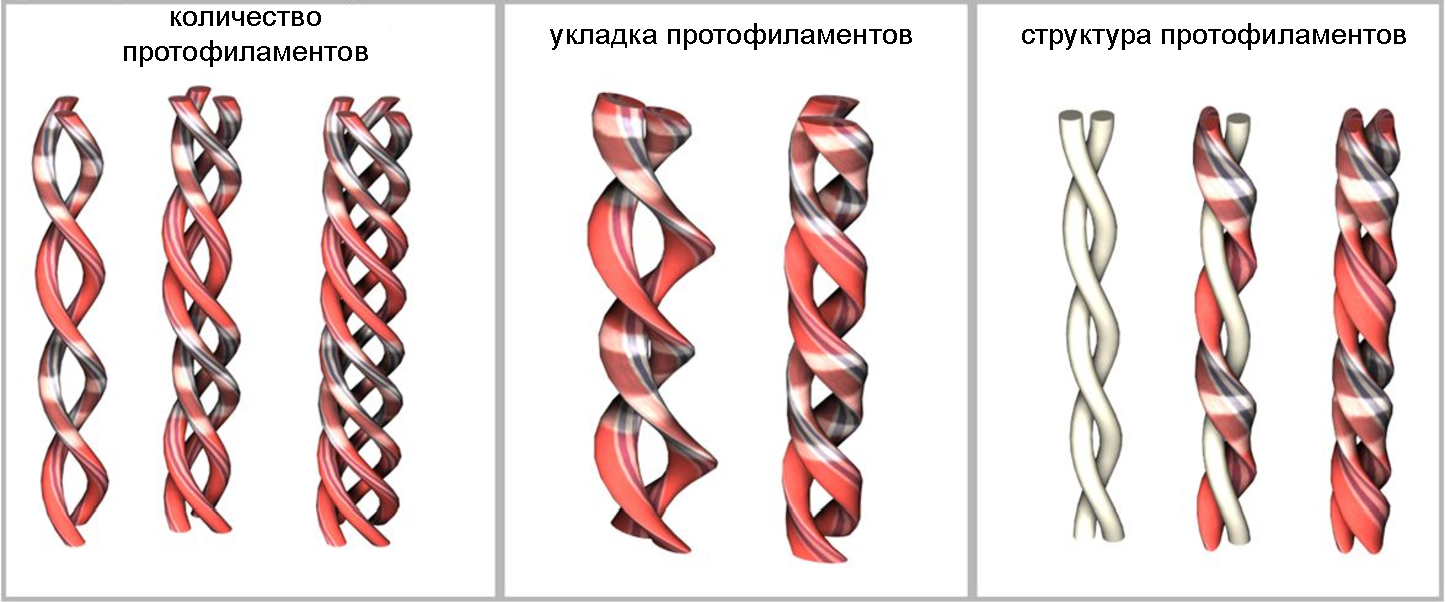
\includegraphics[width=\textwidth]{images/p4/punkt1/part4_p1_f4.pdf}
    \caption[Структурные типы полиморфизма амилоидных фибрилл]{Структурные типы полиморфизма амилоидных фибрилл. Схематическое изображение различных морфологий амилоидных фибрилл, которые различаются количеством, относительной ориентацией или структурой лежащих в основе протофиламентов.}
    \label{fig:p4_p1_f4}
\end{figure}



\subsection{Экспериментальные методы, используемые для изучения амилоидоподобных волокон}

    В настоящее время для изучения амилоидных (-подобных) фибриллярных агрегатов применяется множество различных экспериментальных подходов, включая рентгеновскую и электронную дифракцию, оптическую и электронную микроскопию, АСМ, твердотельный ЯМР, рассеяние нейтронов, ИК, УФ-видимую и КД спектроскопию, связывание красителей в сочетании со сложной подготовкой и модификацией фибрилл и агрегирующих молекул.
    
    В то время как химическая структура агрегирующих соединений почти всегда известна, а морфология фибрилл в субмикронном масштабе решается с помощью электронной или атомно-силовой микроскопии, структура фибрилл в атомистическом и наноразмерном масштабах, включая упаковку отдельных молекул, очень часто остается недоступной для возможностей экспериментальных измерений. В конкретных случаях становится возможным получить представление о внутренней структуре фибрилл, когда могут быть получены соответствующие микрокристаллы (с помощью дифракции рентгеновских лучей) или когда доступны достаточные данные ЯМР. Однако эти данные, хотя и бесценно полезны, до сих пор ограничиваются лишь несколькими небольшими пептидами при определенных условиях. Для большинства соединений и, более того, для полимер-биоконъюгатов имеющиеся экспериментальные данные о межмолекулярных взаимодействиях в большинстве случаев ограничиваются спектроскопическим анализом (ИК, УФ-видимая, КД-спектроскопия) и характерными дифракционными картинами (рентгеновские лучи, электроны) и, следовательно, точное структурное расположение в наномасштабе и его связь с морфологией остаются плохо понятными.
    
\subsection{Самосборка и образование фибрилл}

    Большое внимание уделяется раскрытию механизма образования амилоидных фибрилл, поскольку понимание механизмов, лежащих в основе полимеризации растворимого мономерного пептида в зрелые нерастворимые фибриллы, может пролить свет на возможные терапевтические подходы к остановке, обращению или предотвращению образования фибрилл. Процесс образования амилоидных фибрилл, по-видимому, начинается с частично структурированных конформеров белков \cite{uversky_conformational_2004,kelly_alternative_1998}. Частичное сворачивание/разворачивание белков, по-видимому, способствует определенным межмолекулярным взаимодействиям, таким как гидрофобные и электростатические взаимодействия, которые необходимы для стимулирования полимеризации белковых молекул в амилоидные фибриллы. Это термодинамически неблагоприятное состояние затем переходит в стабильную амилоидогенную форму.
    
    Для некоторых белков предлагается модель полимеризации зависящей от нуклеации при описания образования фибрилл, аналогичная описанию процесса кристаллизации \cite{come_kinetic_1993}. Гетерогенное ядро (``затравка'') или пептидная мицелла формируется выше критической ``пороговой'' концентрации, и фибриллы зарождаются внутри них, удлиняясь за счет необратимого связывания мономеров со своими свободными концами \cite{lomakin_nucleation_1996,walsh_amyloid_1999}. Рост фибрилл может быть представлен схематически в виде кривой экспоненциального роста с отставанием, где фаза значительно укорачивается в присутствии затравок.
    
    Однако становится все более очевидным, что для многих белков такие модели не подходят для извлечения информации о размере ядра из зависимости кинетики образования амилоидных фибрилл от концентрации белка \cite{xue_systematic_2008}. В случае образования амилоидных фибрилл многими белками наблюдается быстрое образование сферических олигомеров и/или протофибрилл, и во многих случаях зрелые фибриллы появляются при длительной инкубации \cite{s_conformational_2008,mukhopadhyay_characterization_2006,apetri_secondary_2006,chimon_evidence_2007,goldsbury_multiple_2005,jain_evidence_2008,kumar_mechanism_2007}. Этот механизм агрегации получил название ``сборка с помощью олигомерных промежуточных продуктов'' \cite{s_conformational_2008,serio_nucleated_2000,modler_assembly_2003}. В этом механизме, по-видимому, образование префибриллярных агрегатов не ограничивается неблагоприятным событием нуклеации \cite{jain_evidence_2008,kumar_mechanism_2007,hurshman_transthyretin_2004} и может рассматриваться как изодесмическая полимеризация \cite{hurshman_transthyretin_2004}.
    
    Начальная фаза образования фибрилл многими белками характеризуется накоплением сферических олигомеров и протофибрилл. Электронная микроскопия и эксперименты с атомно-силовой микроскопией показывают, что самые ранние префибриллярные агрегаты представляют собой сферические олигомеры \cite{s_conformational_2008,mukhopadhyay_characterization_2006,apetri_secondary_2006,jain_evidence_2008,kumar_mechanism_2007,serio_nucleated_2000,modler_assembly_2003,hurshman_transthyretin_2004,carrotta_protofibril_2005,kad_hierarchical_2003}, которые впоследствии, по-видимому, сливаются с образованием гранулированных удлиненных червеобразных амилоидных протофибрилл. Удлиненные протофибриллы иногда могут округляться с образованием кольцевых, кольцевидных протофибрилл \cite{lashuel_alpha-synuclein_2002,lashuel_neurodegenerative_2002,kayed_annular_2009}. Недавно было показано, что кольцевые протофибриллы белка амилоид-$\beta$ структурно отличаются от сферических олигомеров; они обнаруживают эпитоп, который отсутствует в сферических олигомерах и в фибриллах белка \cite{kayed_annular_2009}. Альтернативно, образование фибрилл может идти по ``пути смещения'' без образования фибрилл, но вместо этого включает превращение промежуточных продуктов в аморфные отложения \cite{rambaran_amyloid_2008}.
    
    Важно определить, когда происходит конформационная конверсия $\beta$-листа во время образования амилоидных фибрилл. В реакциях образования амилоидных фибрилл, демонстрирующих характерные особенности механизма подобного кристаллизации, и в большинстве примеров сборки через олигомерные промежуточные соединения, рост агрегатов и приобретение $\beta$-листовой структуры, по-видимому, связаны \cite{jain_evidence_2008,kumar_mechanism_2007,serio_nucleated_2000,modler_assembly_2003,esler_alzheimers_2000,scheibel_elongation_2004}. Похоже, что связывающие звенья (мономеры или олигомеры) сначала присоединяются к концам растущих агрегатов, а затем претерпевают конформационные изменения $\beta$-слоя. Недавно для двух белков было замечено, что образование амилоидных фибрилл включает конформационно преобразованные олигомерные промежуточные соединения, т.е. конформационные изменения $\beta$-складок происходят в олигомерных промежуточных соединениях до того, как они присоединяются к концам растущих агрегатов \cite{chimon_evidence_2007}.
    
    Процесс образования амилоидных волокон является относительно медленным, олигомеризация белка амилоида-$\beta$ \textit{in vitro} занимает до 72 часов, прежде чем отдельные фибриллы могут быть разделены \cite{chimon_evidence_2007}.
    
    Отличительным признаком самосборки амилоида является наличие иерархии различных взаимодействий, которые управляют фибриллярной структурой и морфологией на разных уровнях организации: например, $\beta$-листы -> ``стерические застежки-молнии'' -> протофиламенты -> амилоидные волокна. Хотя взаимодействие между различными межмолекулярными взаимодействиями и его влияние на морфологию довольно сложно и не до конца изучено, Aggeli et al. предложили хорошую статистико-механическую модель, подкрепленную экспериментальными данными, которая очерчивает основные уровни иерархии и доминирующие межмолекулярные взаимодействия \cite{aggeli_hierarchical_2001}. Модель описывает самосборку хиральных стержнеобразных единиц, таких как пептиды, образующие $\beta$-листы, в спиральные ленты, которые с увеличением концентрации объединяются в скрученные ленты (двойные ленты), фибриллы (скрученные стопки лент) и волокна (переплетенные фибриллы) (см. рисунок \ref{fig:p4_p1_f5}). Показано, что конечная ширина и спиральность фибриллы являются результатом конкуренции между приростом свободной энергии от притяжения между лентами и проигрышем в энергии из-за упругого искажения внутренне скрученных лент при включении в растущую фибриллу. Волокна стабилизируются аналогично. Поведение двух рационально сконструированных пептидов из 11 остатков аминокислот, P11-I и P11-II, иллюстрирует предложенную схему. P11-I и P11-II предназначены для принятия конформации $\beta$-нити и для самосборки в одном измерении с образованием антипараллельных $\beta$-листовых лент, двойных лент, фибрилл и волокон в четко определенных растворителем условиях.

\begin{figure} [H]
    \centering
    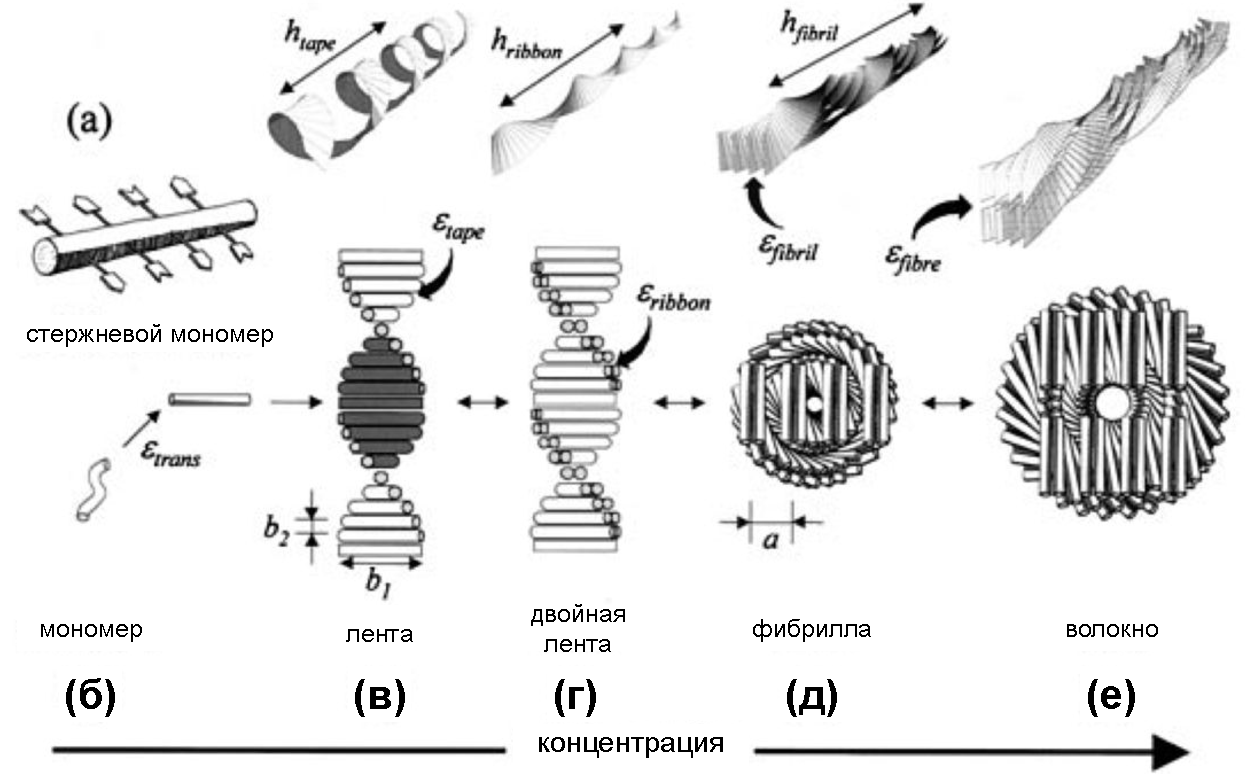
\includegraphics[width=\textwidth]{images/p4/punkt1/part4_p1_f5.pdf}
    \caption[Модель иерархической самосборки хиральных стержневых единиц]{Модель иерархической самосборки хиральных стержневых единиц. Локальные расположения (в–е) и соответствующие глобальные равновесные конформации для иерархических самособирающихся структур, сформированных в растворах хиральных молекул (a), которые имеют дополнительные донорные и акцепторные группы, показанные стрелками, через которые они взаимодействуют и выравниваются, образуя ленты (в). Черная и белая поверхности стержня (а) отображены на сторонах спиральной ленты (в), которая выбрана так, чтобы закручиваться к черной стороне (в). Все внешние стороны двойной ленты (г), фибриллы (д) и волокна (е) белые. Одна из фибрилл в волокне (е) для ясности нарисована более темным оттенком. (д и е) Вид спереди краев фибрилл и волокон соответственно. Адаптированно из Aggeli et al. \cite{aggeli_hierarchical_2001}.}
    \label{fig:p4_p1_f5}
\end{figure}





\subsection{Функциональные амилоиды и синтетические амилоидные агрегаты}

    Однако амилоидные фибриллы не всегда вредны. Сейчас все чаще становится очевидным, что живые организмы, от прокариот до людей, используют амилоидные фибриллы, образованные их эндогенными белками, для выполнения нормальных физиологических функций \cite{chiti_protein_2006,fowler_functional_2006}. Многие грибы производят амфипатические белки, называемые гидрофобинами \cite{sunde_structural_2008}. Они обладают способностью собираться в фибриллы, богатые $\beta$-слоями, на границах раздела воздух-вода, и считается, что они играют защитную роль в грибковых структурах, таких как споры и плодовые тела. Предполагается, что прионы дрожжей играют функциональную роль, формируя цитоплазматические фибриллярные сборки, которые могут быть связаны с методом наследственной передачи информации \cite{uptain_prions_2002}. Амилоидные и амилоидоподобные фибриллярные агрегаты, образованные природными белками или синтетическими пептидами и полимерными биоконъюгатами, привлекают большое внимание как из-за их возможного применения в качестве строительных блоков в нано- и биотехнологиях. Амилоидные фибриллы все чаще исследуются на предмет их потенциальной роли в формировании нанотрубчатых (и не только) каркасов для бионанотехнологий \cite{scheibel_conducting_2003,hamada_engineering_2004,hamedi_electrochemical_2008}. Сами фибриллы могут быть очень прочными, имеющими такую же прочность на растяжение, как сталь \cite{smith_characterization_2006}, свойство, которое они разделяют со своим структурным родственником, шелком. Пептидные волокна можно функционализировать путем присоединения белков \cite{baldwin_cytochrome_2006} или использовать в качестве матрицы для связывания с металлами \cite{scheibel_conducting_2003,reches_casting_2003}.
    
    Болдуин и др. \cite{baldwin_cytochrome_2006} собрали гибридный белок, состоящий из функционального цитохрома b562 с амилоидогенной последовательностью SH3. Структуры имели амилоидоподобное ядро, при этом обладали функциональными свойствами глобулярного цитохрома. Другой пример - нанопроволоки, которые в одной из работ были изготовлены путем сборки белков, таких как N-терминальная область дрожжевого приона Sup35. Конъюгированные частицы коллоидного золота были связаны вдоль волокон с использованием открытых остатков цистеина  Sup35, в результате чего были получены проволочки диаметром около 100 нм \cite{scheibel_conducting_2003}. В другой работе очень короткий пептид, состоящий из двух остатков фенилаланина, собирается с образованием амилоидоподобных нанотрубок, которые можно функционализировать с помощью ионнов серебра в центре нанотрубки. В результате были получены нанопроволоки диаметром около 20 нм \cite{reches_casting_2003}.
    
    Другой подход, привлекающий все большее внимание, - это синтетическое конъюгация пептидов с другими молекулярными соединениями. Конъюгаты синтетических и природных макромолекул представляют большой интерес в настоящее время из-за их многообещающих биомедицинских, микроэлектронных и других передовых технологических приложений \cite{borner_strategies_2009,lutz_modern_2008,borner_bioinspired_2007,vandermeulen_peptideprotein_2004,hardy_silk-inspired_2009,schlaad_block_2003}. Ковалентное присоединение синтетических полимеров к амилоидогенным пептидным последовательностям приводит к новому классу блок-сополимеров, которые могут унаследовать типичные свойства своих составляющих, например улучшенные рабочие характеристики, проводимость, биосовместимость и высокую склонность к самоорганизации. Обзоры \cite{borner_strategies_2009,lutz_modern_2008,borner_bioinspired_2007,vandermeulen_peptideprotein_2004} обобщают последние достижения в области химии биоконъюгации полимеров, из которых биоконъюгирование с амилоидогенными пептидами является одним из наиболее часто используемых. На результирующее взаимодействие межмолекулярных взаимодействий влияют как синтетические, так и пептидные части, что приводит к еще большему структурному полиморфизму, чем наблюдается в природных амилоидных волокнах, имея в виду, что синтетическая химия обеспечивает большую вариативность в структуре строительных блоков, включая разветвленные молекулярные топологии \cite{eckhardt_rational_2005}. Ряд предполагаемых самоорганизующихся морфологий, которые могут быть адаптированы различными полимерными биоконъюгатами, изображены на рисунке \ref{fig:p4_p1_f6}. Более того, взаимодействие между различными взаимодействиями может также указывать на зависимость супрамолекулярной организации от внешних условий (таких как температура, качество растворителя, pH и др.), что перспективно для технологических приложений \cite{ikkala_hierarchical_2004}.

\begin{figure} [H]
    \centering
    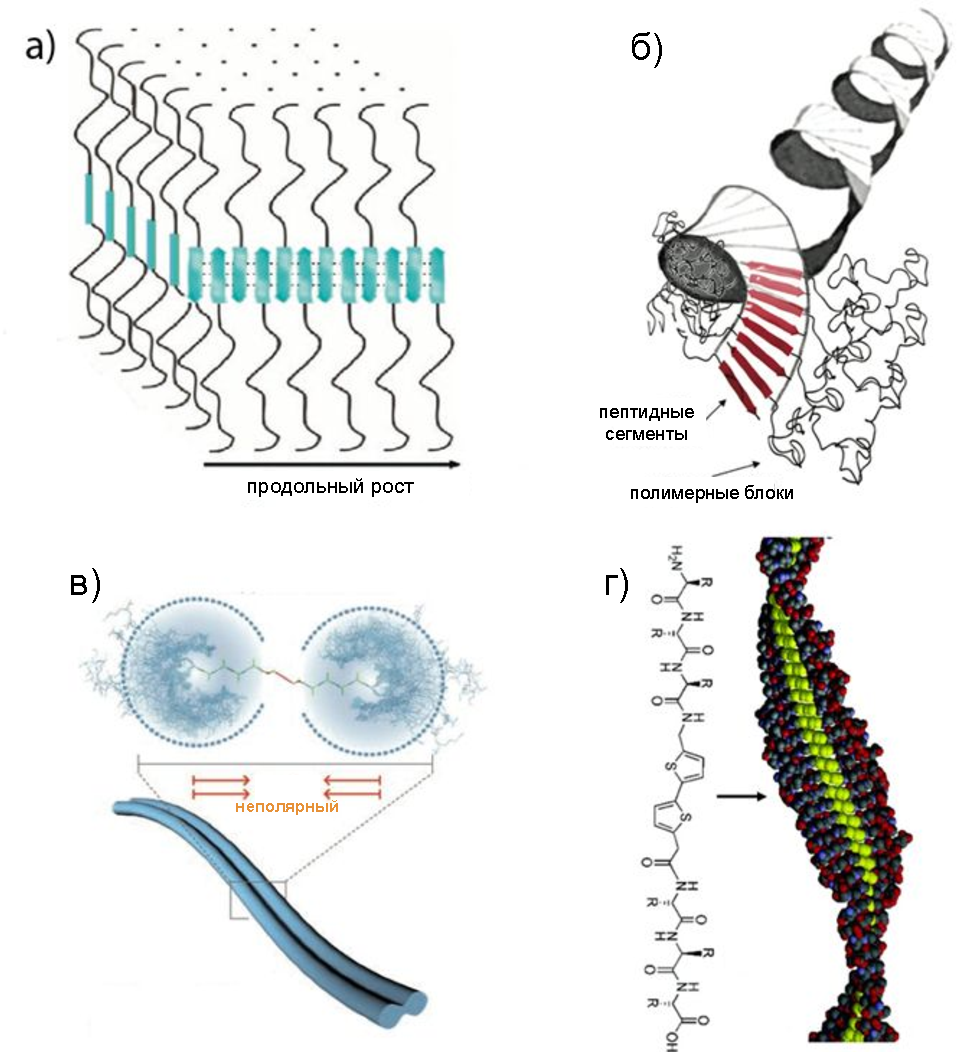
\includegraphics[width=\textwidth]{images/p4/punkt1/part4_p1_f6.pdf}
    \caption[Примеры различных морфологической организации фибриллярных агрегатов, предположительно образуемых полимерными биоконъюгатами]{Примеры различных морфологической организации фибриллярных агрегатов, предположительно образуемых полимерными биоконъюгатами: (а) широкие плоские ленты \cite{hentschel_switch-peptides_2006}, (б) спиральная надстройка \cite{hentschel_peptide-directed_2006}, (в) ленты с поперечным сечением в форме гантели \cite{frauenrath_general_2008}, (г) спиральные ленты с полимером посередине \cite{diegelmann_one-dimensional_2008}. По материалам \cite{diegelmann_one-dimensional_2008,hentschel_switch-peptides_2006,hentschel_peptide-directed_2006,frauenrath_general_2008}.}
    \label{fig:p4_p1_f6}
\end{figure}



\subsubsection{Конъюгаты тиофен-пептид}

    Как подчеркивалось ранее, ярким примером конъюгатов пептид-полимер являются конъюгаты пептидов, образующих $\beta$-лист, и электропроводящих полимеров - тиофенов, которые, как было показано, образуют фибриллы как в воде \cite{diegelmann_one-dimensional_2008}, так и в органических средах \cite{schillinger_oligothiophene_2009}. Примеры синтетических ``молекулярных химер'', в которых одна часть молекулы состоит из олиготиофена, а другая - из аминокислотной последовательности, образующей $\beta$-лист, были представлены несколькими группами. Klock et al. \cite{klok_synthesis_2004} синтезировали молекулу типа TP, в которой кватро(3-гексилтиофен) (T) функционализирован пентапептидной последовательностью Gly-Ala-Gly-Ala-Gly (P), которая, как известно, образует $\beta$-листовые домены в шелке тутового шелкопряда (см. рис. \ref{fig:p4_p1_f7}а, а'). Эти авторы обнаружили образование длинных линейных цепей шириной от 3,5 до 4,0 нм и высотой 3\AA{} на поверхности из молекул TP и тенденцию пептидных блоков к формированию $\beta$-листов посредством множественных водородных связей. Однако точная архитектура наблюдаемой сверхструктуры еще не известна, и детальная схема водородных связей еще не может быть нарисована. Schillinger et al. \cite{schillinger_oligothiophene_2009} провели исследование симметрично замещенного P-T-P-алкилированного гибрида кватротиофен-пептида, который включает последовательность $(Thr-Val)_3$, которая, как известно, имеет высокую склонность к принятию $\beta$-листовой формы (см. рис. \ref{fig:p4_p1_f7}б, б’). АСМ и ПЭМ снова указали на образование волокнистых структур длиной до 1-2 мм (АСМ), высотой 2,4 $\pm$ 0,4 нм (АСМ) и шириной 8 $\pm$ 2 нм (ПЭМ) и 11 $\pm$ 2 нм (АСМ). Diegelmann et al. \cite{diegelmann_one-dimensional_2008} сообщили об успешном синтезе битиофенов, присоединенных к последовательностям Ala-Phe-Glu-Gln-Gln и Glu-Phe-Ala-Gln-Glu (гибрид типа P-T-P) (см. рис. \ref{fig:p4_p1_f7}в, в’). Атомно-силовая микроскопия (АСМ) образцов гелей, нанесенных на слюду, выявила одномерные наноструктуры высотой от 2 до 6 нм. Еще два примера гибридов олиготиофеновых пептидов были представлены Ступпом и сотрудниками. Первоначально был представлен гибрид тертиофена, который включает одну глутаминовую кислоту и два блока аланина \cite{tsai_self-assembly_2008}. В дальнейшем этот подход был расширен до двух производных центрального пентатиофена, симметрично замещенных двумя последовательностями Lys-Lys-Leu-Leu \cite{stone_self-assembling_2009} (см. рис. \ref{fig:p4_p1_f7}г, г’). Обнаруженные наноструктуры имели ширину 4,94 $\pm$ 0,76 нм.
    
    Во всех исследованиях с помощью атомно-силовой микроскопии было визуализировано, что при определенных условиях эти соединения могут самоорганизовываться в длинные (в диапазоне микрометров) морфологически похожие фибриллярные агрегаты с шириной фибриллы, обычно варьирующейся от 4 до 50 нм и высотой от 0,3. до 6 нм. Однако взаимосвязь между молекулярным составом, молекулярной конформацией, межмолекулярными силами и трехмерной супрамолекулярной организацией этих материалов мало изучена. Следовательно, необходимы дополнительные экспериментальные и теоретические исследования, чтобы вывести структурную модель, описывающую расположение этих гибридов на основе олиготиофена-олигопептида.

\begin{figure} [H]
    \centering
    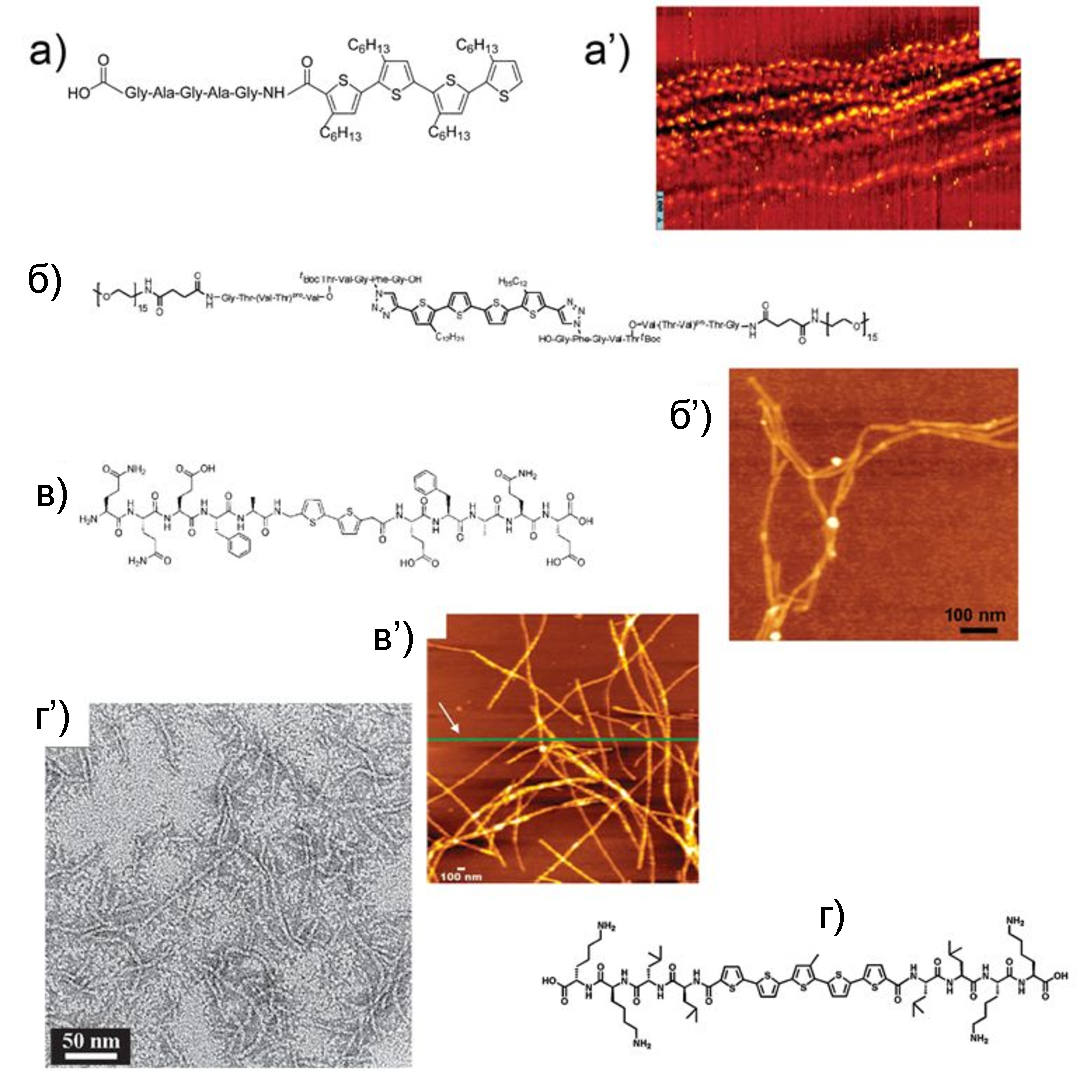
\includegraphics[width=\textwidth]{images/p4/punkt1/part4_p1_f7.pdf}
    \caption[Различные конъюгаты тиофенов и пептидов, образующих $\beta$-лист]{Различные конъюгаты тиофенов и пептидов, образующих $\beta$-лист, и соответствующие изображения наблюдаемых фибриллярных агрегатов с помощью АСМ или ПЭМ. По материалам  \cite{diegelmann_one-dimensional_2008,klok_synthesis_2004,schillinger_oligothiophene_2009,stone_self-assembling_2009}.}
    \label{fig:p4_p1_f7}
\end{figure}



\subsubsection{Диблок-олигомер кватротиофена и пептида}

    В настоящем разделе мы опишем экспериментальные данные, доступные для самосборки диблочного олигомера кватротиофен-$\beta$-листовой пептида (изображенного на рисунке \ref{fig:p4_p1_f1}). Представленные здесь данные были получены от группы профессора Бойерле, университет г. Ульма.
%возможно, не нужно чтобы картинка тут отображалась, но понятия не имею как это сделать, поэтому пока что закоментил ее(выше ссылка на нее ((\ref{fig:p4_p1_f1})))
%\begin{figure} [H]
%    \centering
%    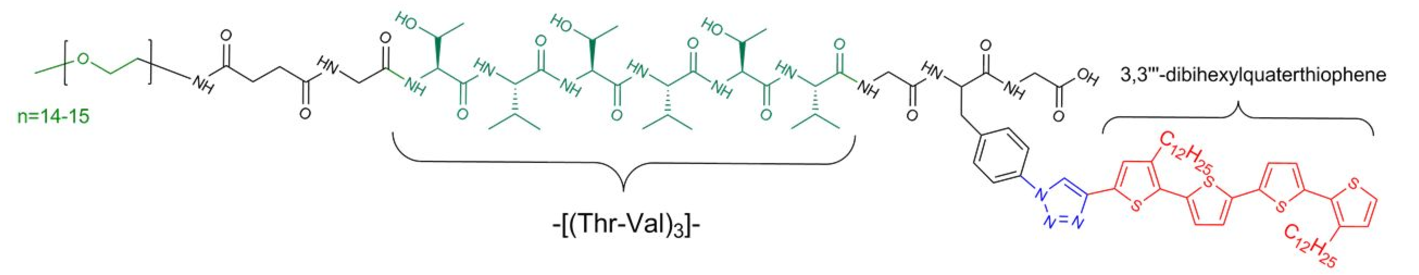
\includegraphics[width=\textwidth]{images/p4/punkt1/part4_p1_f1.pdf}
%    \caption{Структурная формула диблок-олигомера алкилированного кватротиофен-$\beta$-листового пептида, функционализированного PEO, включающего три повтора последовательности Thr-Val.}
%    \label{fig:p4_p1_f1}
%\end{figure}

    \textbf{Гибридный дизайн}. Гибридное соединение Т-P (рис. \ref{fig:p4_p1_f1}) было разработано путем комбинации симметрично дидодецил-замещенного кватротиофена, функционализированного с одной стороны конъюгатом ПЭГ-$\beta$-пептид. Последовательность пептида включает три повтора Val и Thr. Ранее было показано, что используемый кватротиофен самособирается в очень регулярные сверхструктуры на границе раздела жидкость-твердое тело (АСМ) и в объеме (дифракция рентгеновских лучей) \cite{azumi_coincidence_2000,bauerle_oligothiophenes_1995,mena-osteritz_superstructures_2002}. Известно, что повторы $(Val-Thr)_x$ образуют стабильные $\beta$-листы в водных и органических средах \cite{janek_water-soluble_1999,hentschel_switch-peptides_2006,hentschel_peptide-directed_2006}.
    
    Такие последовательности, образующие $\beta$-лист, известны как ``сложные последовательности'' \cite{eckhardt_rational_2005,hentschel_peptide-guided_2007}, потому что они имеют тенденцию к агрегированию во время синтеза и обработки. Были реализованы две стратегии, чтобы обойти такую нежелательную агрегацию и в дополнение к получению контроля над процессом самосборки. Во-первых, в пептид была включена так называемая псевдопролиновая единица, которая после кислотного снятия защиты превращается в повтор Val-Thr \cite{wohr_pseudo-prolines_1996}. Во-вторых, использовали фрагмент переключающегося сложного эфира, который вызывает временный дефект в природной амидной цепи за счет введения связи $\beta$-сложного эфира между $Val^5$ и $Thr^6$ \cite{sohma_novel_2004,mutter_switch_2004,carpino_synthesis_2004}. Дефект переключателя сохраняется в кислых условиях, но нативный амидный остов может быть восстановлен путем увеличения pH, тем самым вызывая перегруппировку в звене переключателя сложного эфира (перенос O-> N-ацила) (см. Рисунок \ref{fig:p4_p1_f8}). Для лучшей гибкости полученного гибрида между пара-азидофенилаланином и последовательностью $\beta$-листа был введен глицин, потенциально разрушающий вторичную структуру. В конце концов, гибрид был снабжен ПЭГ-цепью на N-конце, чтобы повысить растворимость и предотвратить потенциальные латеральные взаимодействия фибриллярных агрегатов.

\begin{figure} [H]
    \centering
    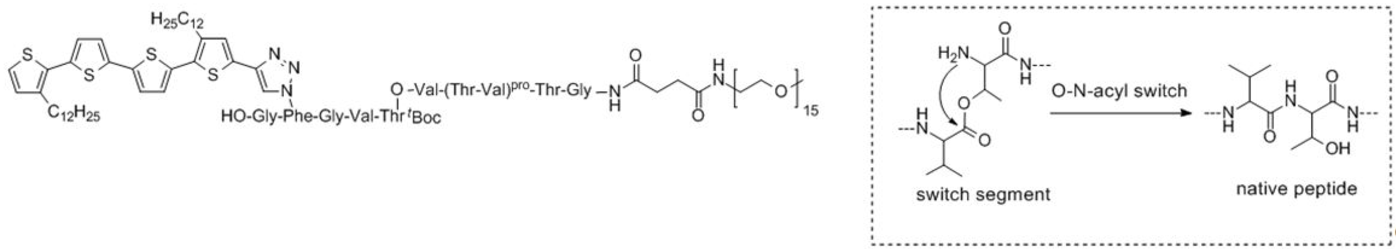
\includegraphics[width=\textwidth]{images/p4/punkt1/part4_p1_f8.pdf}
    \caption[Синтезированное соединение Т-P в ``защищенной'' форме]{Синтезированное соединение Т-P в ``защищенной'' форме. На вставке показан переключатель O-N-ацила, который срабатывает при повышении pH.}
    \label{fig:p4_p1_f8}
\end{figure}

    Чтобы способствовать превращению нарушенных пептидных сегментов гибрида (рис. \ref{fig:p4_p1_f8}) в нативные $\beta$-цепи, был выбран контролируемый подход путем добавления 0,001 М гидроксида натрия, растворенного в метаноле, к ранее приготовленному раствору в дихлорметане (ДХМ) с помощью шприцевого насоса до тех пор, пока не будет достигнуто соотношение растворителей 1:1. Наличие полностью протяженной последовательности $\beta$-листов было доказано с помощью ИК-спектроскопии. В ИК-Фурье спектре отсутствие полос для интактного фрагмента сложного эфира переключателя ($\nu = 1785 см^{-1}$ и $\nu = 1743 см^{-1}$) сопровождается сдвигом полосы амида I в область, специфичную для $\beta$-листа ($\nu = 1636 см^{-1}$), что указывает на присутствие полностью протяженной пептидной структуры, которая участвует в формировании вторичной структуры $\beta$-слоя. Из-за довольно широкой формы полосы амида I для гибрида во вторичной структуре $\beta$-слоя было, к сожалению, невозможно однозначно определить, антипараллельная (специфическая полоса при $\nu = 1690 см^{-1}$) или параллельная (отсутствие эта полоса) пептидных цепей присутствует в $\beta$-листе.
    
    \textbf{Самосборка}. Для несимметричного гибрида ПЭГ-$\beta$-пептид-олиготиофен исследовали самосборку на поверхности и в растворе. Принимая во внимание различную полярность гибрида (доминирующие гидрофобные взаимодействия со стороны олиготиофена, водородные связи пептидного сегмента) и сильную тенденцию к агрегации $\beta$-листового пептида в его нативной форме, для самосборки была выбрана стратегия на основе изменения свойств растворителя, использующая шприцевой насос, для одновременной перестройки пептидного остова и самосборки гибрида \cite{schillinger_oligothiophene_2009}.

\begin{figure} [H]
    \centering
    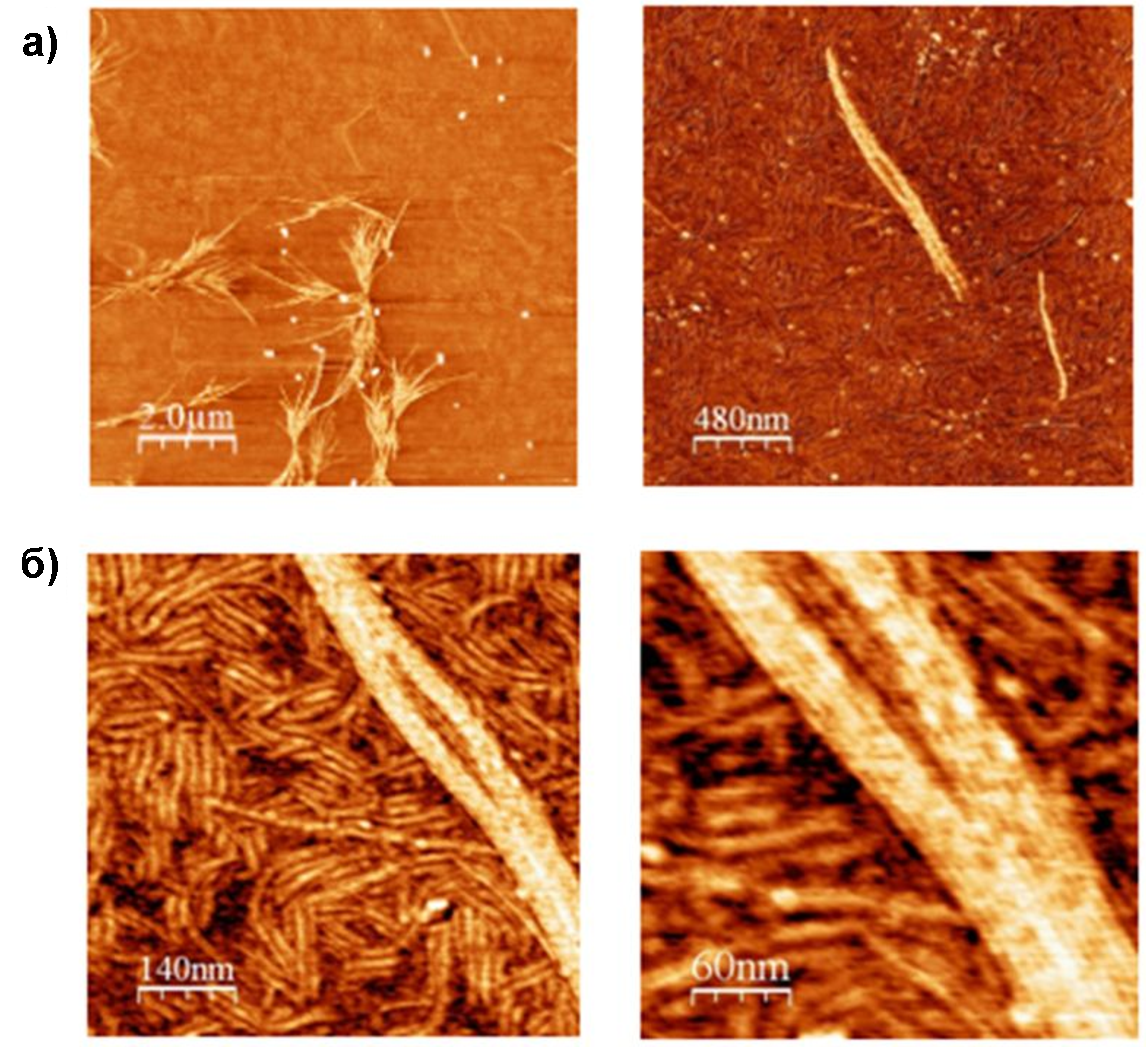
\includegraphics[width=\textwidth]{images/p4/punkt1/part4_p1_f9.pdf}
    \caption[АСМ изображения высоты и фазы нативного ПЭГ-пептида-кватротиофена]{АСМ изображения высоты и фазы нативного ПЭГ-пептида-кватротиофена, нанесенного центрифугированием на слюду из смеси ДХМ/0,001 М NaOH в МеОН, раствор 1:1, приготовленный с помощью шприцевого насоса; а) Высотные изображения АСМ: слева: пучки волокон, полученные через 7 дней, справа: одиночное волокно; б) Фазовые изображения АСМ, слева и справа: увеличенное изображение одного волокна, показывающее состав большего волокна из мелких волокон. Предоставлено Евой-Катрин Шиллингер, группой профессора П. Бойерле.}
    \label{fig:p4_p1_f9}
\end{figure}

    С помощью АСМ волокна были обнаружены в образце с центрифугированием на подложке из мусковитовой слюды (рис. \ref{fig:p4_p1_f9}). Изображения были получены в тэппинг режиме после стабилизации адсорбата в течение нескольких дней. Можно было визуализировать скопление волокон, рисунок которых не соответствует сети, а больше напоминает кластеры (рис. \ref{fig:p4_p1_f9}а, слева). Вокруг этих больших участков концентрированного материала можно найти одиночные ``более крупные'' волокна (рис. \ref{fig:p4_p1_f9}а, слева и справа). Можно показать, что эти более крупные волокна представляют собой пучки нескольких более тонких волокон разной длины, выровненных параллельно (рис. \ref{fig:p4_p1_f9}б, оба изображения), что объясняет нерегулярный вид более крупных отдельных волокон, которые мы поэтому называем пучками. Кроме того, короткие фибриллярные структуры, окружающие пучки, регулярно откладываются на поверхности слюды (рис. \ref{fig:p4_p1_f9}б). Эти короткие фибриллярные структуры можно рассматривать как самые маленькие одиночные структуры, которые затем иерархически самоорганизуются в более крупные структуры (пучки или даже кластеры).
    
    Размер пучков колеблется от 1 до 2 мкм в длину, от 1 нм $\pm$ 0,2 нм в высоты и от 15 до 48 нм в ширину, хотя также могут наблюдаться спорадические ширины примерно до 80 нм. Самая маленькая самособирающаяся единица на слюдяной подложке (вышеупомянутые короткие фибриллярные структуры, которые предположительно являются однослойными $\beta$-листами) имеет длину от 100 до 500 нм и повторяющуюся ширину 7 нм $\pm$ 2 нм и высоту 0,5 $\pm$ 0,2 нм. Несоответствие размеров пучков, особенно ширины, считается результатом предложенной иерархической самосборки, которая ведет от одиночных $\beta$-листов (наименьшие наблюдаемые фибриллярные структуры) к двойным лентам, то есть двухслойным $\beta$-листам (отдельные волокна в пучке), которые, в свою очередь, взаимодействуют по бокам, образуя пучки.
    
    В просвечивающей электронной микроскопии (ПЭМ) наблюдались структуры, очень похожие на структуры, исследованные с помощью АСМ.

    Поскольку фибриллярные объекты можно было наблюдать с помощью АСМ на слюде после центрифугирования, а также в ПЭМ после нанесения методом drop casting на покрытые углеродом медные сетки, можно предположить, что эти нано- и микроструктуры уже присутствуют в растворе, и преобладающие эффекты подложки на самосборке маловероятны \cite{schillinger_oligothiophene_2009}. Как упоминалось ранее, также кватротиофеновая часть в гибриде, представленном здесь, способна самоорганизовываться за счет $\pi - \pi$-стэкинга и ван-дер-ваальсовых взаимодействий \cite{azumi_coincidence_2000,bauerle_oligothiophenes_1995,mena-osteritz_superstructures_2002}. Следовательно, потенциальная роль $\pi - \pi$ взаимодействий в конечной самоорганизующейся супраструктуре была исследована методами УФ-видимой, флуоресцентной и КД-спектроскопии.
    
    Однако флуоресцентная спектроскопия, как очень чувствительный метод, не выявила какой-либо агрегации, которая непосредственно влияет на $\pi$-систему. С помощью спектроскопии КД не удалось получить никаких указаний на хиральное экситонное взаимодействие сопряженных $\pi$-систем кватротиофенов. Однако очень слабый неотмеченный сигнал в спектре КД при энергиях ниже максимума поглощения сопряженной $\pi$-системы указывал на существование хромофорных агрегатов в хиральном окружении.



\section{Мультимасштабное интегративное моделирование фибрилл из тиофен-пептидных олигомеров}

    В настоящем разделе мы представляем комплексное моделирование фибриллярных агрегатов из диблочных олигомеров кватротиофена и $\beta$-листового пептида, основанное на различных предполагаемых межмолекулярных структурах, инспирированных структурами родственных амилоидных фибрилл. Мы выполняем мультимасштабное исследование, которое состоит из \cite{schopf_polythiophenes_1997} предсказания различных межмолекулярных структур, \cite{garten_light-emitting_1996} моделирования коротких фибрилл в явном растворителе, \cite{choi_polymers_2008} моделирования длинных фибрилл в вакууме, \cite{cai_polymer_2009} моделирования фибрилл на графитовой подложке. Мы описываем комбинированный интгративный экспериментальный/теоретический подход, направленный на определение структуры и свойств амилоидоподобных фибриллярных агрегатов.

\subsection{Формулировка задачи}

    Было обнаружено, что симметрично дидодецилзамещенный кватротиофен, функционализированный с одной стороны конъюгатом ПЭГ-$\beta$-пептид (см. Рисунок \ref{fig:p4_p1_f1}), самособирается в фибриллярные агрегаты в растворе, которые были визуализированы с помощью ПЭМ и АСМ (см. рис. \ref{fig:p4_p1_f9}). Внутренняя структура агрегатов не разрешена экспериментальными методами, хотя спектральные данные предполагают, что структура $\beta$-листов формируется в растворе. В этой работе мы стремимся использовать модели молекулярной механики и моделирование молекулярной динамики для изучения возможных моделей организации гибридных молекул тиофен-пептид (Т-P) и установления связей между межмолекулярным расположением и надмолекулярной морфологией фибриллярных агрегатов.

    Поскольку использование одного подхода или методологии было бы недостаточно для решения этой проблемы, мы проводим комплексное многомасштабное исследование этой системы, которое сочетает в себе методы моделирования с доступными экспериментальными данными и рациональным пониманием иерархии взаимодействий при самосборке. Наше исследование состоит из следующих этапов: (i) построение модели молекулярной механики TP-соединения и предложение различных межмолекулярных структур, согласующихся с экспериментальными данными и общими принципами образования амилоидных волокон, (ii) оптимизация структуры и оценка этих молекулярных расположений проводится с помощью МД-моделирования одномерных периодических кристаллов, (iii) из выбранных периодических расположений строятся короткие фибриллы ($\sim 10$ нм в длину), которые моделируются в явном органическом растворителе, (iv) более длинные фибриллы ($\sim 40$ нм в длину) моделируются в вакууме и изучается их морфология, (v) выполняется специальное моделирование фибрилл, адсорбированных на графите, для изучения эффектов адсорбции и получения прямого соответствия с данными АСМ.
    
    \begin{figure} [H]
    \centering
    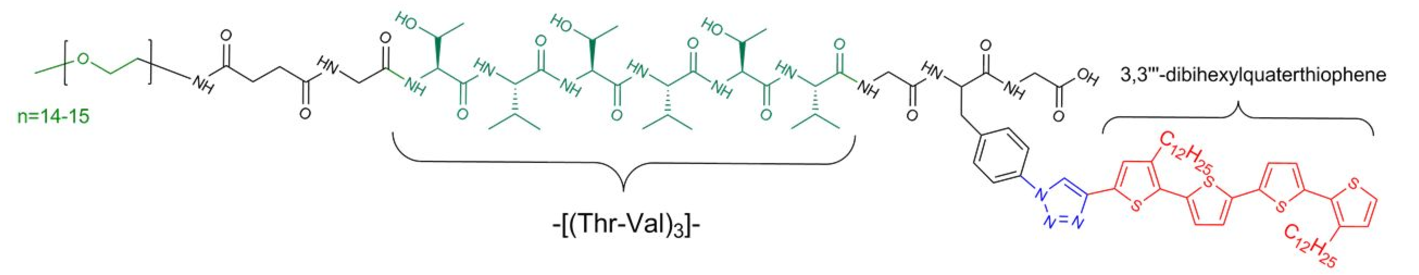
\includegraphics[width=\textwidth]{images/p4/punkt1/part4_p1_f1.pdf}
    \caption[Исследуемое соединение тиофен-пептид]{Исследуемое соединение тиофен-пептид.}
    \label{fig:p4_p1_f1}
\end{figure}
    

\subsection{Молекулярно-механическая модель}

    В качестве отправной точки для теоретического рассмотрения экспериментально наблюдаемых нановолокон была выбрана молекулярная структура гибрида олиготиофен-пептид, как показано на рисунке \ref{fig:p4_p5_f31}, и была построена соответствующая полноатомная модель молекулярной механики. Модельное соединение отличается от экспериментального отсутствием гибкого ПЭГ-хвоста, поскольку ПЭГ-хвост не обладает способностью к определенным межмолекулярным взаимодействиям и первоначально был добавлен в основном по причинам растворимости. Следовательно, на нашем уровне методологии моделирования цепи ПЭГ вряд ли будут играть важную роль, определяющую структуру.

\begin{figure} [H]
    \centering
    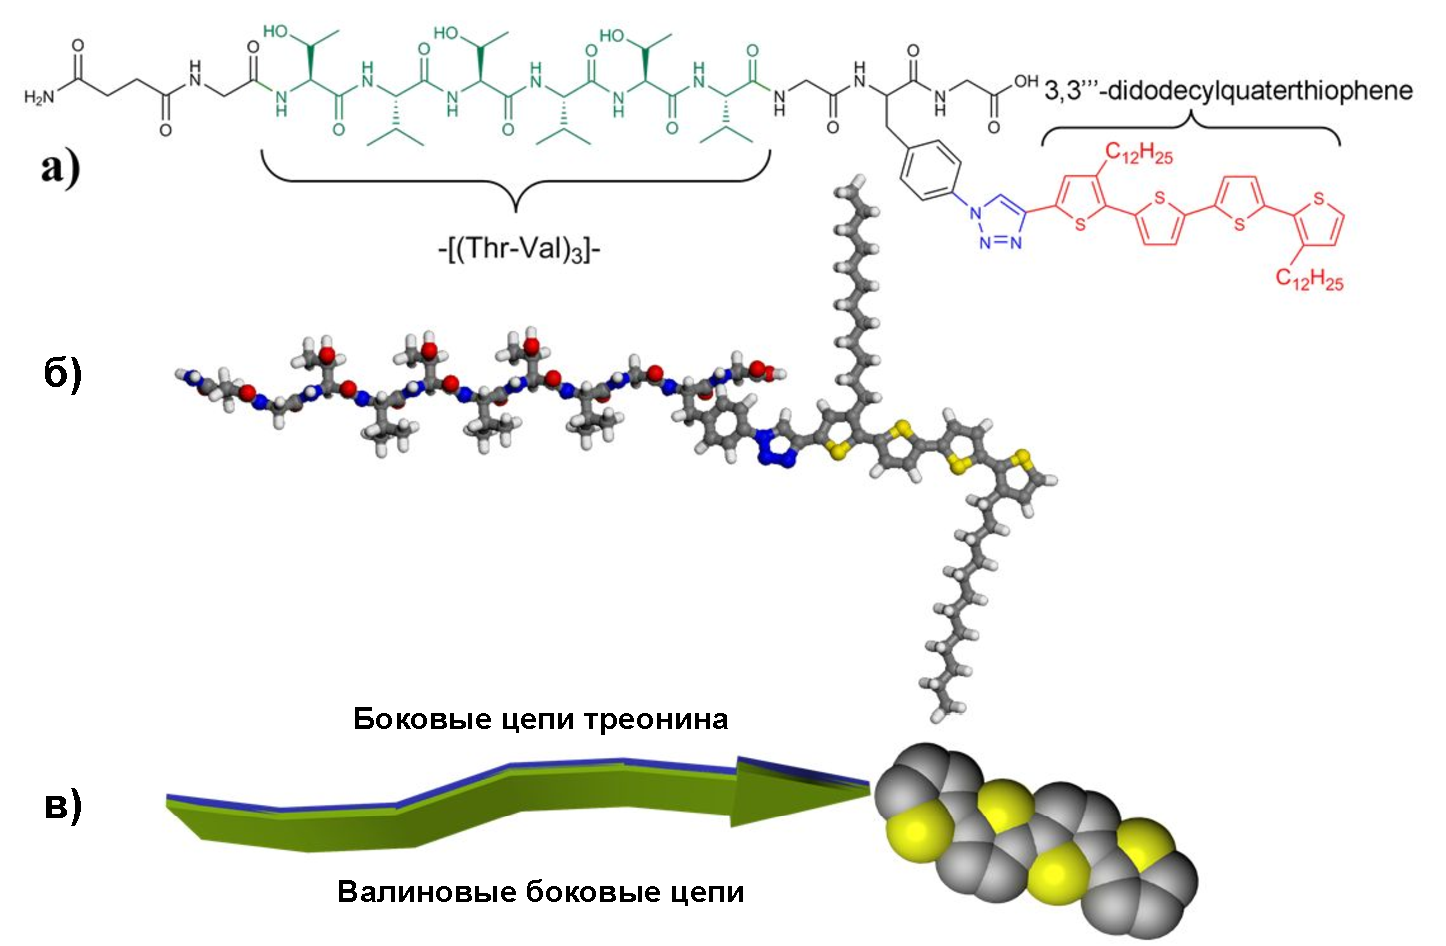
\includegraphics[width=\textwidth]{images/p4/punkt5/part4_p5_f31.pdf}
    \caption[Различные представления молекулы T-P, используемые для компьютерного моделирования самособирающихся фибриллярных агрегатов]{Различные представления молекулы T-P, используемые для компьютерного моделирования самособирающихся фибриллярных агрегатов. a) структурная формула, б) представление всех атомов с конформацией основной цепи, соответствующей конформации $\beta$-нити, в) схематическое представление $\beta$-цепи и кватротиофенового фрагмента.}
    \label{fig:p4_p5_f31}
\end{figure}

    Полноатомная молекулярная модель исследуемого соединения была основана на силовом поле PCFF класса II, параметризованного для воспроизведения \textit{ab initio} энергетических поверхностей \cite{sun_force_1994,maple_derivation_1994,peng_derivation_1997}.

\subsection{Построение и анализ периодических укладок}

    В принципе, обе части гибридной молекулы (конъюгированная часть и пептидная часть) способны к сильным межмолекулярным взаимодействиям, что приводит к образованию сильно анизотропных структур, таких как нановолокна, наностержни и т. д. Поскольку образование волокон в наномасштабе (особенно амилоидоподобных волокон) из $\beta$-листовых пептидов происходит по известному механизму самосборки \cite{ecroyd_crystallin_2009}, подобные пептид-пептидные взаимодействия могут играть определяющую структурную роль для образования супраструктуры нашего гибридного соединения.
    
    Большинство экспериментальных данных, доступных в литературе (включая разрешенные с помощью рентгеновских лучей и ЯМР-спектроскопии структуры амилоидоподобных фибрилл), предполагают, что в биологических амилоидных волокнах основным мотивом структурной агрегации пептидов является соединение длинных $\beta$-нитей в ленты с помощью латерально взаимодействующих одиночных пептидных цепей. Эти ленты могут, в свою очередь, накладываться друг на друга лицом к лицу, образуя фибриллы (филаменты) с так называемой четвертичной структурой с перекрестными $\beta$-ядром, которая считается основной характерной чертой амилоидных фибрилл. Стопки лент могут в дальнейшем взаимодействовать друг с другом и образовывать более толстые нитевидные агрегаты \cite{aggeli_hierarchical_2001}. Однако, если взаимодействие между лентами затруднено, ленты могут скручиваться в спиральные структуры, как это было предложено Aggeli et al. (см. рис. \ref{fig:p4_p1_f5}) на основе их теоретических моделей, подтвержденных экспериментальными наблюдениями \cite{aggeli_hierarchical_2001}, а также обнаруженных в конъюгатах ПЭГ-пептид или поли(бутилакрилат)-пептид или поли(бутадиен)-пептид \cite{hentschel_peptide-directed_2006,jahnke_molecular_2008}. Вопрос о предпочтении параллельного или антипараллельного расположения $\beta$-листов в таких фибриллярных структурах является спорным. Хотя было обнаружено, что многие экспериментально исследованные амилоидоподобные фибриллы имеют параллельное расположение $\beta$-слоев, различные амилоидные фибриллы, которые могут быть удивительно похожими по супрамолекулярной морфологии, могут существенно различаться в молекулярных деталях, включая параллельное или антипараллельное расположение $\beta$-слоев \cite{margittai_fibrils_2008}.

    Исходя из вышеупомянутых идей, связанных со структурной организацией пептидных молекул в нитевидные агрегаты, мы предлагаем несколько периодических расположений для нашего гибридного соединения, исходя из предположения, что пептидная часть соединения организована аналогичным образом. Два предложенных основных периодических механизма включают параллельную или антипараллельную организацию пептидных фрагментов в $\beta$-листах. Еще четыре компоновки были получены из этих однослойных компоновок путем наложения $\beta$-листов лицом к лицу аналогичным структуре некоторых амилоидных фибрилл. Две основные однослойные периодические структуры, основанные на параллельных и антипараллельных $\beta$-листах, были построены с использованием комбинации молекулярного выравнивания и моделирования молекулярной динамики и показаны на рисунке \ref{fig:p4_p5_f32}. Полученные однослойные периодические структуры затем использовались в качестве блоков для образования различных двухслойных конструкций. Мы сконструировали эти двухслойные структуры из уравновешенных однослойных димеров, стремясь имитировать расположение пептидной части, наблюдаемое в амилоидоподобных фибриллярных структурах, разрешенных с помощью дифракции рентгеновских лучей или ЯМР-спектроскопии \cite{nelson_structure_2005,luhrs_3d_2005} с последующей обширной релаксацией. Релаксация методом МД позволяет молекулам регулировать свое периодическое расположение до наилучшего локального минимума свободной энергии.

    Двухслойные структуры были созданы следующим образом: однослойная структура была воспроизведена, повернута на $180^{\circ}$ вокруг оси ленты и затем отрегулирована в латеральной плоскости так, чтобы пептидные сегменты двух однослойных фибрилл были приблизительно равны в регистре, образуя центр гибридной фибриллы. $\beta$-листы внутри такой фибриллы могут взаимодействовать либо с боковыми цепями валина, либо с боковыми цепями треонина каждого листа, обращенными друг к другу. Любое перекрытие молекулярных фрагментов, которое имело место (например, внутри алкильных цепей), разрешалось небольшими корректировками задействованных торсионных углов, которые в любом случае могли бы получить их равновесные значения во время цикла релаксации. Обсуждаемая процедура привела к четырем различным двухслойным периодическим системам, представленным на рисунке \ref{fig:p4_p5_f33}. В принципе для параллельного расположения-нитей можно подумать о двух других двухленточных конформациях с пониженной симметрией, когда $\beta$-цепи в обеих лентах идут параллельно друг другу (см. рисунок \ref{fig:p4_p1_f3}). Однако такие структуры считались маловероятными, поскольку (i) такое структурное расположение $\beta$-нитей не наблюдалось экспериментально до настоящего времени для биологических амилоидных волокон, (ii) такому расположению не будет способствовать взаимодействие дипольных моментов соседних лент, и (iii) только одно такое расположение допустимо стерически из-за громоздкости тиофеновых фрагментов гибридной молекулы.

\begin{figure} [H]
    \centering
    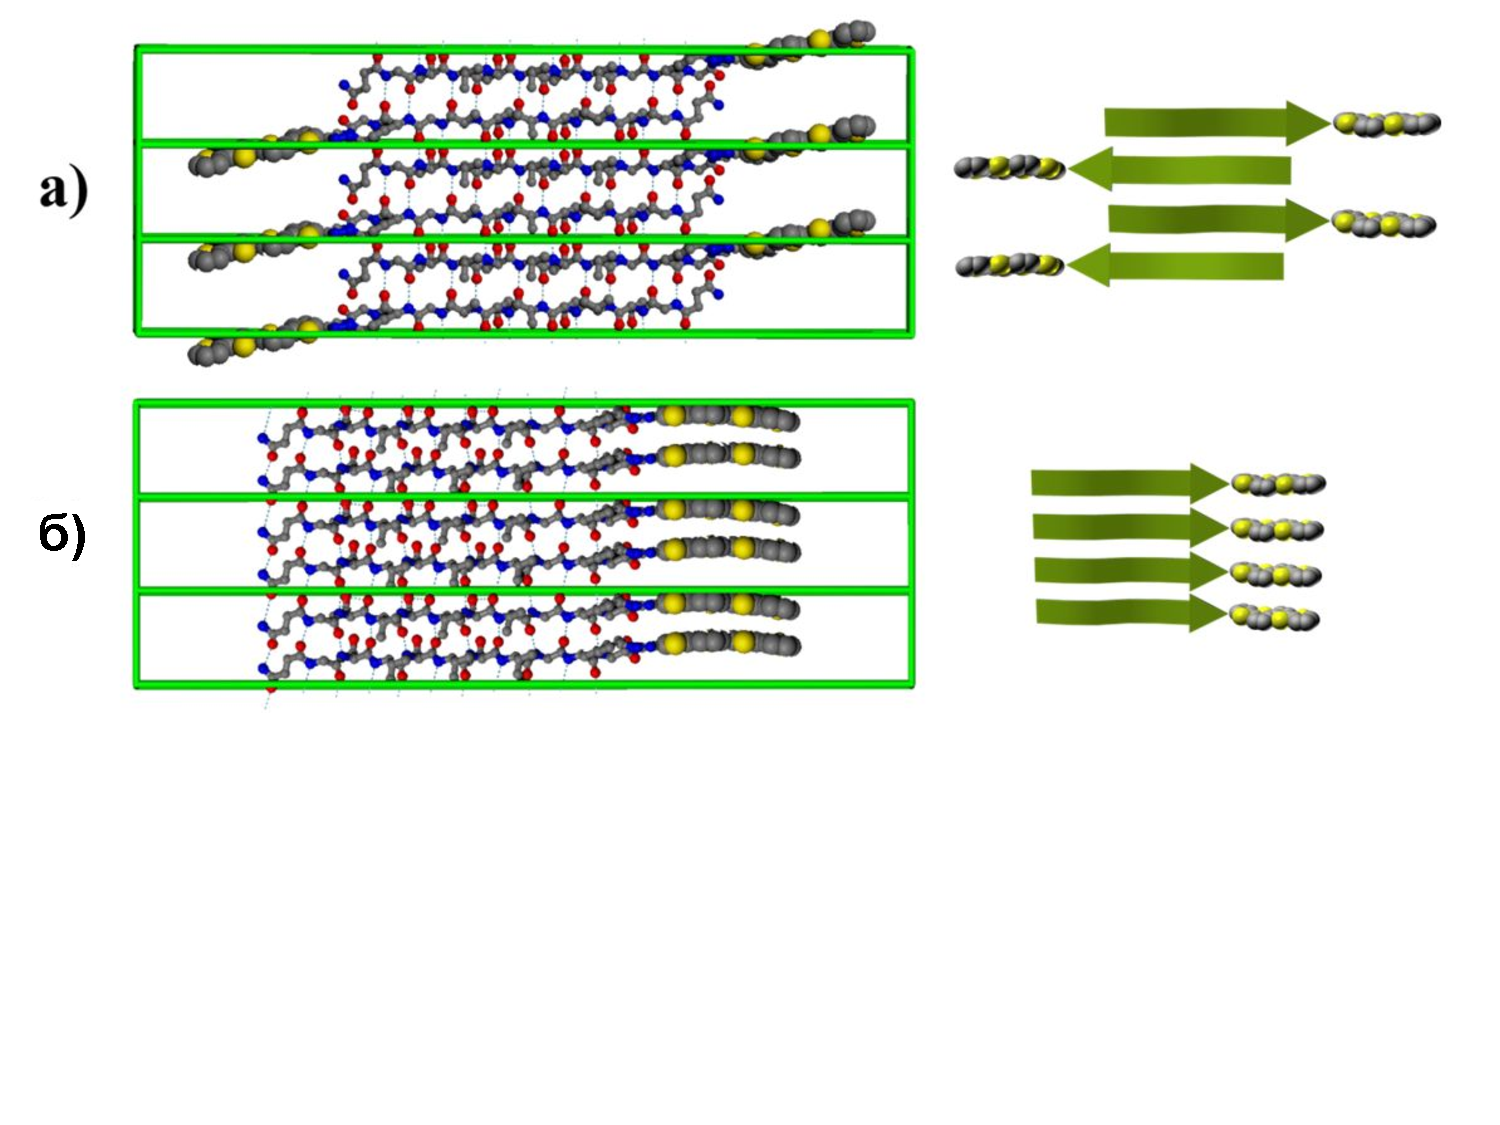
\includegraphics[width=\textwidth]{images/p4/punkt5/part4_p5_f32.pdf}
    \caption[Построенные однослойные периодические  ячейки укладки T-P соединений]{Построенные однослойные периодические  ячейки укладки T-P соединений. Построенные периодические кристаллические ячейки для а) антипараллельного и б) параллельного расположения пептидных цепей в однослойных фибриллах. Алкильные цепи опущены для ясности; пунктирными линиями показаны водородные связи, ответственные за образование $\beta$-листа. На вставках справа показано принципиальное расположение пептидных и тиофеновых фрагментов.}
    \label{fig:p4_p5_f32}
\end{figure}

\begin{figure} [H]
    \centering
    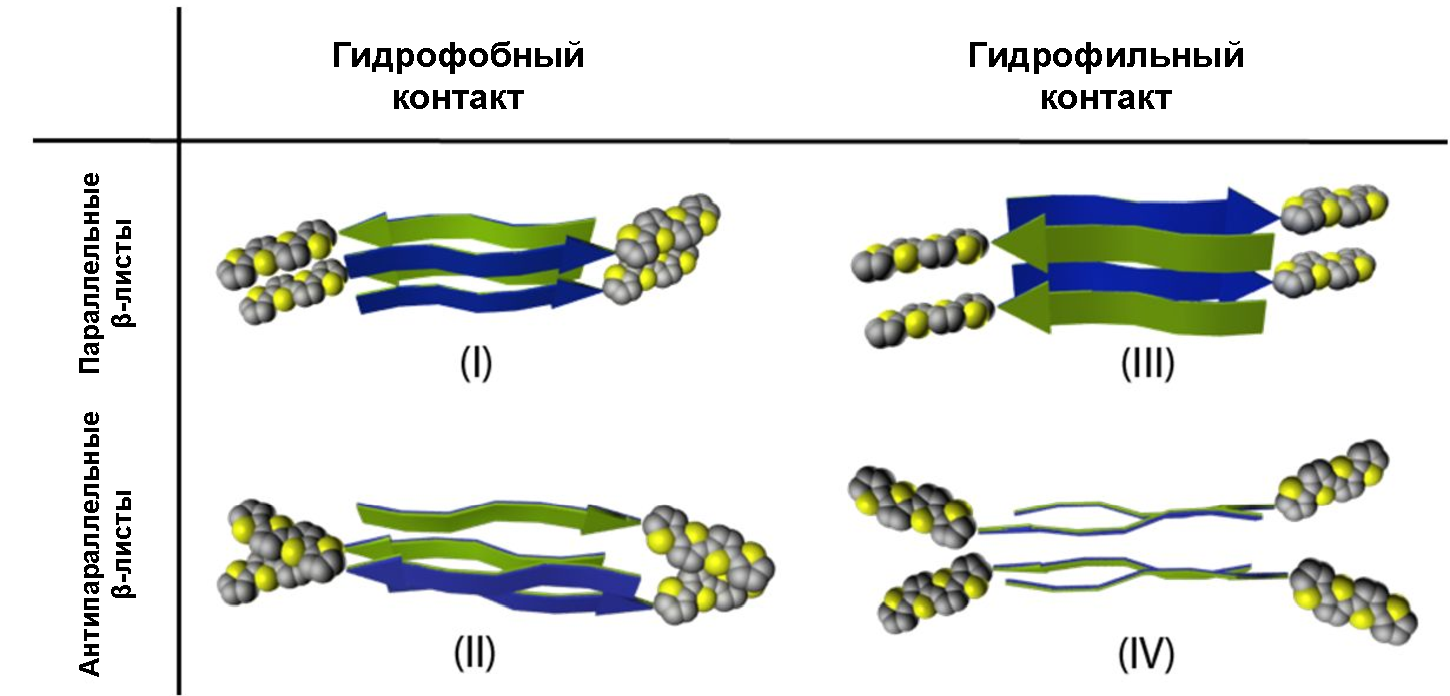
\includegraphics[width=\textwidth]{images/p4/punkt5/part4_p5_f33.pdf}
    \caption[Построенные двухслойные периодические кристаллические ячейки укладки T-P соединений]{Построенные двухслойные периодические  ячейки укладки T-P соединений. Схематические изображения сконструированных двухслойных периодических структур из гибридной молекулы, классифицированные по ориентации $\beta$-листов (параллельная или антипараллельная) и типу межслоевого контакта $\beta$-листов (гидрофобный: валин-валин, гидрофильный: треонин-треонин).}
    \label{fig:p4_p5_f33}
\end{figure}

    Поскольку двойные слои представляют собой значительно более сложные конформационные сборки, особенно в отношении организации поверхностей, скрытых между двумя $\beta$-слоями, и взаимодействия боковых цепей на этих поверхностях, для этих периодических структур был проведен цикл релаксации молекулярной динамики в 10 нс. Во время этого прогона имела место определенная перестройка конформаций боковой цепи между $\beta$-листами.

    Относительные энтальпии образования для всех структур во время эксперимента отслеживались: самая низкая энтальпия образования наблюдалась для структуры (III) (т.е. наиболее энергетически выгодной структуры). По отношению к структуре (III) структуры (I), (II) и (IV) были менее энергетически выгодными и имели более высокие значения энтальпий образования на 11, 6 и 12 ккал/моль на молекулу соответственно (статистическая ошибка: 1-2 ккал/моль). Хотя этот набор данных был получен при моделировании в вакууме и влияние растворителя не учитывалось, он дает ценные количественные данные для понимания иерархии взаимодействий в таких системах и согласуется с гипотезой о контактах между гидрофильными слоями и антипараллельном расположении листов -- факторов, которые приводят к увеличению энтальпии образования. Однако в нашем случае из-за особой геометрии молекул картина агрегации, основанная на антипараллельных $\beta$-слоях и гидрофильном межслоевом контакте (см. Рисунок \ref{fig:p4_p5_f33}, система (IV)), приводит к потере плотной упаковки между тиофеновыми фрагментами и, следовательно, становится энергетически невыгодной. Благодаря специфичности присоединения тиофеновой составляющей к пептиду более плотная упаковка может быть достигнута только за счет конформационных изменений пептидного остова, что, однако, приводит к менее эффективным взаимодействиям между пептидными цепями $\beta$-листа.

    Известно, что стабильность двухслойной структуры в амилоидных фибриллах часто приписывается ``стерической застежке-молнии'', которая образуется на границе раздела $\beta$-листов. Межслойное расположение боковых цепей для систем (II) и (III) показано на рисунке \ref{fig:p4_p5_f34}. Можно видеть, что боковые цепи противоположных $\beta$-листов находятся в тесном стерическом контакте друг с другом.

\begin{figure} [H]
    \centering
    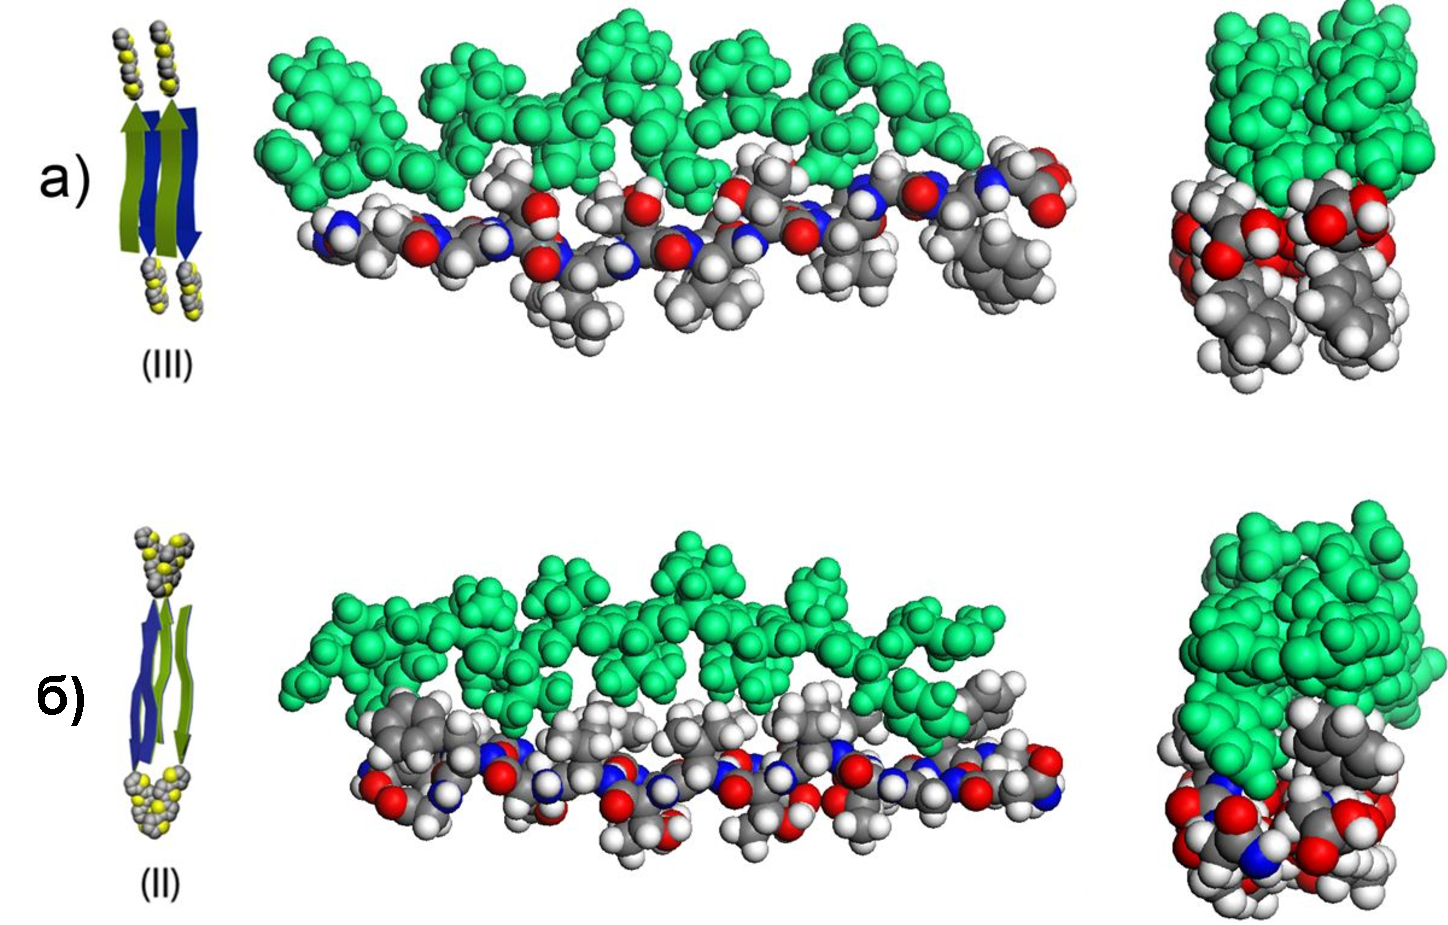
\includegraphics[width=\textwidth]{images/p4/punkt5/part4_p5_f34.pdf}
    \caption[Вид двух двухслойных структур, изображающих интеркаляцию боковых цепей аминокислот, образующих стерическую застежку-молнию]{Вид двух двухслойных структур, изображающих интеркаляцию боковых цепей аминокислот, образующих стерическую застежку-молнию. Кадры делаются после выполнения уравновешивания.}
    \label{fig:p4_p5_f34}
\end{figure}


\subsubsection{Методы и детали}

    Построение однослойных периодических укладок из одиночных молекул осуществлялось с использованием последующих шагов минимизации и релаксации следующим образом.


    Сначала были скорректированы конформации исходных молекул: считалось, что пептидный блок имеет форму-цепи, образующей идеальный параллельный или идеальный антипараллельный $\beta$-лист, который определяется исключительно значениями двугранных $\phi$ и $\psi$ углов пептидного остова, которые, как известно, равны $\phi= -119^{\circ}$,$\psi= -113^{\circ}$ для пептидных цепей параллельного $\beta$-листа и $\phi= -139^{\circ}$,$\psi= -135^{\circ}$ для $\beta$-цепей пептида в антипараллельном $\beta$-листе \cite{nelson_lehninger_2000}. Считается, что тиофеновый блок, включающий боковую цепь 4-азидофенилаланина и алкильные цепи, находится в плоской протяженной конформации, которая соответствует локальному минимуму энергии, как показано на рисунке \ref{fig:p4_p5_f32}б. Чтобы получить правильное периодическое расположение, которое можно было бы использовать в качестве элементарной структуры для построения длинных фибрилл, была получена соответствующая периодическая элементарная ячейка, состоящая из двух (для однослойных фибрилл) или четырех (для двухслойных фибрилл) молекул. Период, предполагаемый элементарной ячейкой вдоль оси фибриллы, был установлен равным 4,8\AA{} на $\beta$-цепь, что соответствует периоду, обычно наблюдаемому в амилоидных фибриллах (9,6\AA\  для двух нитей) \cite{balbach_supramolecular_2002}. На первом этапе две молекулы были организованы в две однослойные периодические структуры с параллельным и антипараллельным расположением $\beta$-цепей, пептидные сегменты в обоих случаях были выровнены так, чтобы максимизировать количество межцепочечных водородных связей (см. Рисунок \ref{fig:p4_p5_f32}). Затем была проведена минимизация энергии для таких периодических однослойных систем (которые можно рассматривать как бесконечно длинные кристаллические ленты) с последующим прогоном релаксационного МД-моделирования длительностью 1 нс.

    Все моделирование проводилось с использованием пакета моделирования LAMMPS \cite{plimpton_fast_1995}. Периодические системы сначала подвергались минимизации энергии с использованием версии Полака-Рибиера алгоритма сопряженного градиента с теми же параметрами силового поля (описанными далее), которые использовались во время моделирования МД. В МД-моделировании периодических систем использовался радиус отсечения для ван-дер-ваальсовых взаимодействий 1,0 нм, кулоновские взаимодействия были учтены с использованием метода PPPM \cite{hockney_computer_1989} с отсечкой 1,0 нм в реальном пространстве и параметром точности $10^{-4}$. Шаг интегрирования составлял 1 фс. Ансамбль NVT с $T=300 K$ поддерживался добавлением трения и стохастических членов к уравнениям движения согласно уравнению Ланжевена, использовалась обратная постоянная трения 1 пс.

\subsection{Моделирование фибриллярных агрегатов в растворителе}

    Как полученные однослойные периодические структуры, так и две из двухслойных структур были использованы для создания коротких фибрилл путем репликации периодической ячейки вдоль оси филамента. Среди двухслойных структур компоновки (II) и (III) были выбраны для дальнейшего изучения, поскольку они (i) представляют собой компоновки с самыми низкими энтальпиями образования среди других и (ii) представляют два различных основных типа расположения $beta$-нитей - параллельную или антипараллельную упаковку, что должно позволить провести интересный сравнительный анализ влияния моделей параллельного или антипараллельного расположения на морфологию и эволюцию волокна. Для выбранных систем были сконструированы плоские прямые фибриллы длиной 20 $\beta$-нитей (приблизительно 40 нм), фибриллы помещались в ячейку с растворителем размером $5x12x10$ нм$^3$. Сам растворитель представлял собой смесь 50\% на 50\% метанола и дихлорметана (по объему), соответствующую той, которая использовалась в эксперименте. Общее количество атомов в системе колебалось в районе 40 тысяч. Эти системы были подвергнуты моделированию МД в течение 10 нс при $T=300 K$, чтобы исследовать их стабильность и проанализировать конформационную релаксацию и поведение.

    Визуальное представление одной из исследуемых систем представлено на рисунке \ref{fig:p4_p5_f35}.

\begin{figure} [H]
    \centering
    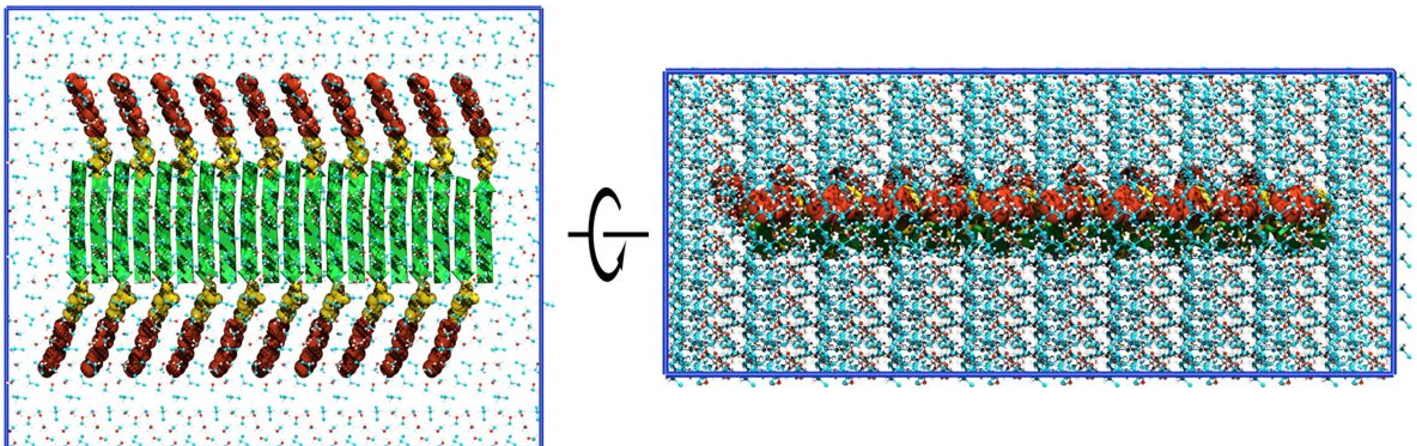
\includegraphics[width=\textwidth]{images/p4/punkt5/part4_p5_f35.pdf}
    \caption[Первоначальный снимок сольватированной короткой однослойной фибриллы на основе антипараллельного расположения $\beta$-листов]{Первоначальный снимок сольватированной короткой однослойной фибриллы на основе антипараллельного расположения $\beta$-листов. Фибрилла визуализируется в комбинированном представлении: пептидные цепи изображены зелеными стрелками, кватротиофен - в изображении атомов, красным, а пара-азидофенилаланиновый линкер - желтым. Алкильные цепи не изображены. Молекулы растворителя (метанол и дихлорметан) показаны точками.}
    \label{fig:p4_p5_f35}
\end{figure}


\subsubsection{Результаты}

    \textbf{Конформационная эволюция}

    Во время моделирования все фибриллы оказались стабильными молекулярными агрегатами, и никакого отрыва молекул от агрегата не наблюдалось, хотя начальная конформация коротких фибрилл изменилась, чтобы принять наиболее энергетически выгодную конформацию. Кадры исходной геометрии фибрилл, а также их снимки после 10 нс времени моделирования представлены на рисунке \ref{fig:p4_p5_f36}. Представленные четыре типа фибрилл будут далее обозначаться их аббревиатурами: SL-AP (однослойная фибрилла, основанная на антипараллельном расположении $\beta$-нитей, изображенная на рисунке \ref{fig:p4_p5_f36}a), AL-PAR (однослойная фибрилла, основанная на параллельном расположении $\beta$-нитей, изображенная на рисунке \ref{fig:p4_p5_f36}б), DL-AP (двухслойная фибрилла, основанная на антипараллельном расположении $\beta$-нитей, тип (II) в обозначениях рис. \ref{fig:p4_p5_f33}, изображенная на рис. \ref{fig:p4_p5_f36}в), DL-PAR (двухслойная фибрилла, основанная на параллельном расположении $\beta$-нитей, тип (III) в обозначениях рис. \ref{fig:p4_p5_f33}, изображенная на рис. \ref{fig:p4_p5_f36}г).

    Однослойные фибриллы имеют тенденцию быть более конформационно гибкими, чем двухслойные фибриллы, как видно из графиков расстояния от конца до конца на рисунке \ref{fig:p4_p5_f36}, где расстояние между центрами масс молекул, находящихся на двух концах фибрилл, изображена как функция времени.
    
    Фибрилла SL-AP после моделирования продемонстрировала левостороннее осевое скручивание пептидного остова с некоторыми намеками на скручивание фибриллы таким образом, чтобы гидрофильная сторона ленты (с открытыми остатками треонина) находилась на вогнутой стороне и гидрофобный (с открытыми боковыми цепями валина) на выпуклой стороне ленты (см. рис. \ref{fig:p4_p5_f36}а).

    Для фибриллы SL-PAR также присутствует осевое левостороннее скручивание, которое сочетается со скручиванием фибриллы, которое имеет тенденцию принимать менее прямую конформацию, что также видно на графике расстояния от конца до конца (см. рис. \ref{fig:p4_p5_f36}б). Фибрилла SL-PAR также менее устойчива на концах, видно, что строгий узор водородных связей $\beta$-листа нарушен на одном конце. Топология завитка такая же, как и у фибриллы SL-AP (гидрофильная сторона ленты находится на вогнутой стороне).
    
    Двухслойные фибриллы имеют тенденцию быть более жесткими и прямыми. В то время как фибрилла DL-AP почти плоская, фибрилла DL-PAR образует выраженный левосторонний осевой поворот на $90^{\circ}$, что соответствует примерно $4,5^{\circ}$ на $\beta$-нить.
    
    Целесообразно сравнить окончательные конфигурации фибрилл с моделями, предложенными Aggeli et al. (см. рисунок \ref{fig:p4_p1_f5}). В обозначениях рисунка \ref{fig:p4_p1_f5} наблюдаемые фибриллы можно разделить на следующие типы: SL-AP и SL-AP - тип (в) - ленты, DL-AP и DL-PAR - тип (г) - двойные ленты.

\begin{figure} [H]
    \centering
    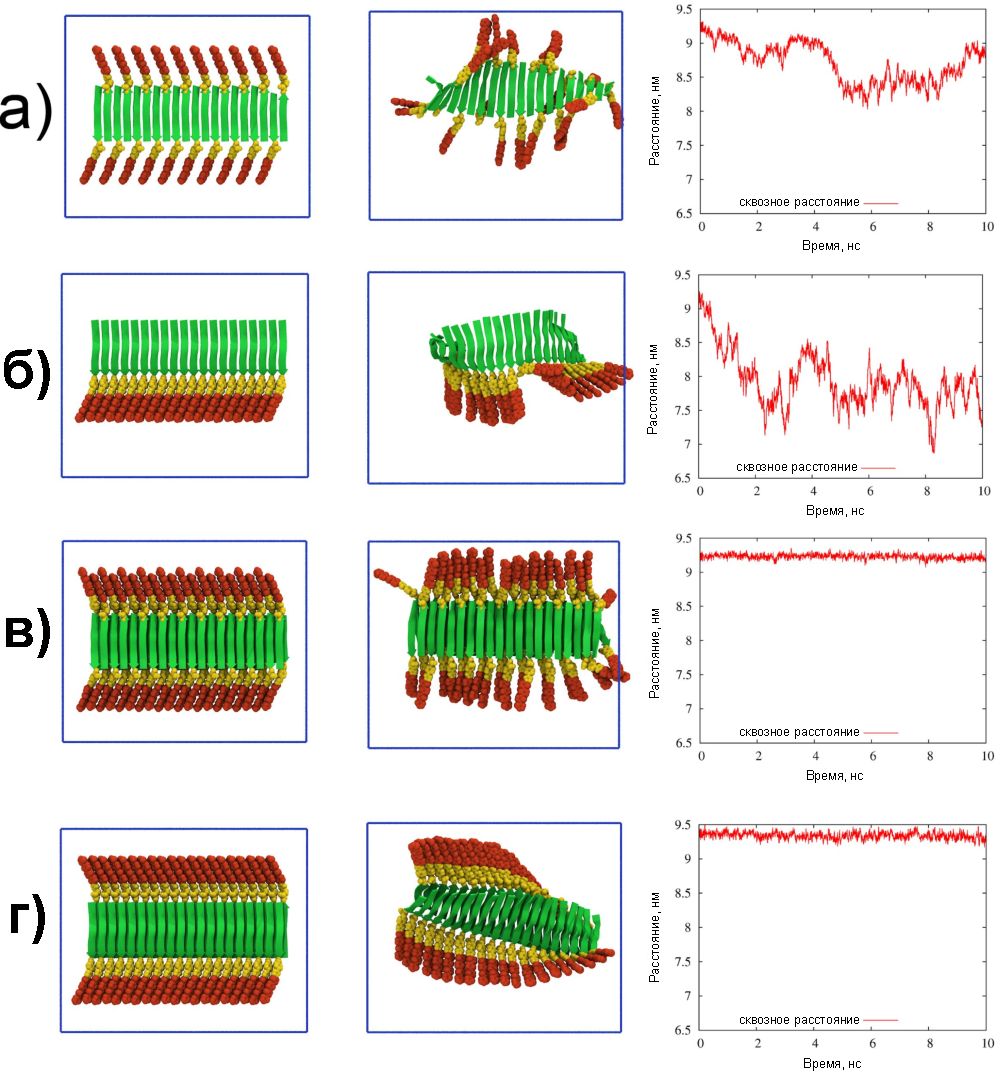
\includegraphics[width=\textwidth]{images/p4/punkt5/part4_p5_f36.pdf}
    \caption[Кадр из моделирования коротких фибрилл в растворителе после 10 нс моделирования]{Кадр из моделирования коротких фибрилл в растворителе после 10 нс моделирования. Фибриллы на основе одиночных $\beta$-листов: а) антипараллельный-лист (SL-AP), б) параллельный $\beta$-лист (SL-PAR). Фибриллы на основе двухслойных $\beta$-листов: в) структура типа (II) на основе антипараллельного $\beta$-листа (DL-AP), г) структура типа (III) на основе параллельного $\beta$-листа (DL-PAR). Алкильные хвосты не изображены, тиофеновая часть изображена красными сферами, пара-азидофенилаланиновый линкер изображен желтым цветом, пептидные части изображены зелеными стрелками. В третьем столбце приведены графики расстояния между центрами масс краевых молекул.}
    \label{fig:p4_p5_f36}
\end{figure}

    Конформационная эволюция может быть дополнительно выявлена, глядя на графики среднеквадратичного отклонения (RMSD) пептидных и тиофеновых фрагментов в фибриллах на рисунке \ref{fig:p4_p5_f37}. RMSD рассчитывали относительно исходной конформации фибриллы по формуле $RMSD = min_{rot,trans} \sqrt{\frac{\sum_{i=1}^{N}|\vec{r_i}(t)-\vec{r_i}(0)|^2}{N}}$, где N - число атомов, $\vec{r_i}(t)$- радиус-векторы атомов, предварительно вычисляется минимум функции по поворотам и трансляциям структуры.
    
    Ясно видно, что флуктуации RMSD для пептидных фрагментов намного меньше для двухслойных структур, чем для однослойных. Начальный дрейф RMSD в течение первых 3-4 нс моделирования связан с конформационной перестройкой пептидных и тиофеновых фрагментов. Например, для фибриллы DL-PAR графики RMSD (рис. \ref{fig:p4_p5_f37}г) четко иллюстрируют скручивание фибриллы.

\begin{figure} [H]
    \centering
    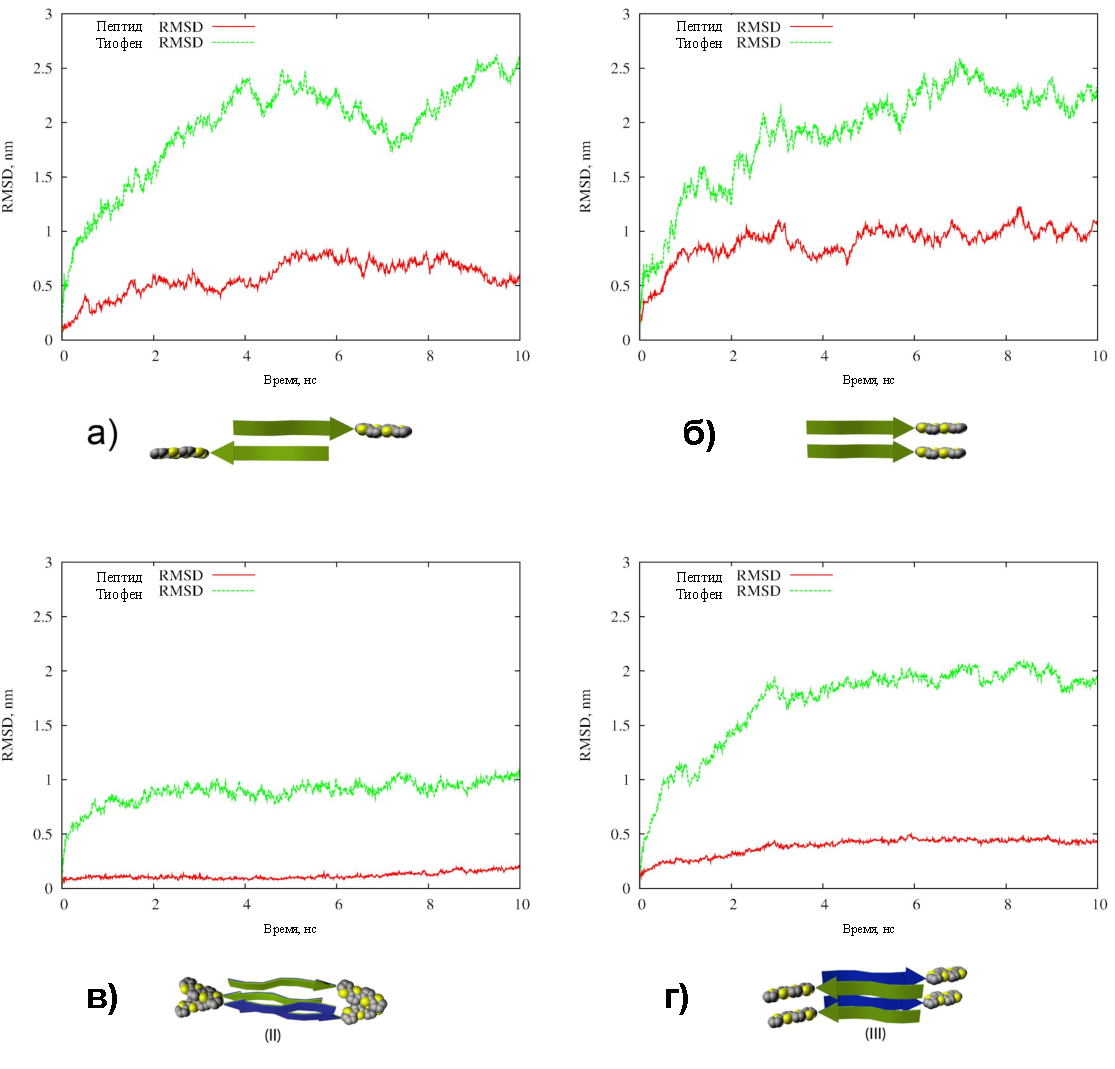
\includegraphics[width=\textwidth]{images/p4/punkt5/part4_p5_f37.pdf}
    \caption[Среднеквадратичное отклонение структуры фибрилл относительно исходной структуры в зависимости от времени моделирования]{Среднеквадратичное отклонение структуры фибрилл относительно исходной структуры в зависимости от времени моделирования.}
    \label{fig:p4_p5_f37}
\end{figure}


    \textbf{Водородные связи}

    Далее мы проанализируем роль водородных связей в стабильности фибрилл. В таблице \ref{tab:p4_t1} и на рисунке \ref{fig:p4_p5_f38} представлены данные по водородным связям для различных типов фибрилл. Известно, что водородные связи являются основным взаимодействием при формировании $\beta$-листа. Каждый остаток в $\beta$-листе обычно образует 2 водородные связи с остатками в следующей $\beta$-нити. Таким образом, максимальное количество водородных связей, которое может образовывать последовательность $[Thr-Val]_3$, которая, как считается, является основным звеном, стоящим за образованием $\beta$-листа, равно 12, или, если рассчитывать на одну молекулу, - 6 (поскольку каждая H- связь принадлежит 2 молекулам). Однако другие группы в гибридной молекуле, такие как боковые цепи треонина (ОН-группа) и другие линкерные аминокислоты (глицин, фенилаланин) и концевые группы, также могут образовывать Н-связи в нашей молекуле. Поскольку точное определение водородной связи может влиять на абсолютные значения водородных связей, мы лучше сосредоточимся на сравнительном анализе водородных связей в различных типах фибрилл.

    Известный факт, что антипараллельные $\beta$-листы имеют тенденцию к образованию более прямых и прочных водородных связей \cite{lehninger_lehninger_2008}, подтверждает вычисленное количество межфибрильных водородных связей для различных типов фибрилл. В то время как антипараллельные фибриллы имеют около 3,3-3,5 водородных связей на гибридную молекулу, параллельные - 2,1-2,5. Из графиков временной эволюции (рис. \ref{fig:p4_p5_f38}) видно, что для того, чтобы произошла конформационная релаксация структуры водородных связей, требуется приблизительно 2 нс.

    Если сравнить фибриллы SL-AP и DL-AP, мы увидим, что для DL-AP наблюдается увеличение межфибрильных водродных связей (3,3 против 3,5), которое компенсируется уменьшением водородных связей фибрилла-растворитель (2,5 против 2,2 ). Это можно рассматривать как следствие большей регулярности упаковки пептидов в двухслойных структурах. Для фибрилл на основе параллельных $\beta$-слоев тенденция аналогична, но гораздо большее уменьшение водродных связей фибрилла-растворитель можно отнести к другому факту: все боковые цепи треонина, содержащие гидроксильную группу, указывают на одну и ту же сторону $\beta$-листа, в фибрилле SL-PAR эти ОН-группы, вероятно, образуют водородные связи с молекулами метанола. Но в фибрилле DL-PAR эти группы ограничены слоями двух соседних $\beta$-листов и имеют меньше возможностей для образования водородных связей.

    Последнее наблюдение, по сути, важно для понимания энергетических проблем образования двухслойных фибрилл. Однослойный $\beta$-лист имеет в нашем случае гидрофобные и гидрофильные стороны, и, образуя двухслойные фибриллы, они могут склеиваться либо с гидрофобными, либо с гидрофильными сторонами, как показано на рисунке \ref{fig:p4_p5_f33}. Гидрофобные или гидрофильные взаимодействия фактически опосредуются растворителем и общее количество водородных связей, которые система имеет в той или иной конформации, является грубой мерой энергетической выгодности гидрофобной или гидрофильной укладки $\beta$-листов. В обсуждаемом случае фибриллы DL-PAR кажется, что гидрофильная укладка $\beta$-листов, хотя и энергетически выгодна сама по себе, не является благоприятной в присутствии растворителя, поскольку гидроксильные группы остатков треонина могут образовывать больше водородных связей при наличии растворителя.

    По общему количеству водродных связей фибрилла DL-AP превосходит все другие фибриллы и, таким образом, вероятно, энергетически более выгодна, чем другие типы фибрилл.

%TABLE1---------------------------------------------------------
\begin{table}[H]
    \centering
    \begin{tabularx}{\textwidth}{|X|X|X|X|}
    Тип фибриллы & Межфибрильные водородные связи на молекулу & Н-связей фибрилла-растворитель на молекулу & Всего Н-связей одна молекула составляет \\
    \hline
    SL-AP  & 3.3 & 2.5 & 9.1\\
    \hline
    SL-PAR & 2.1 & 2.9 & 7.1\\
    \hline
    DL-AP  & 3.5 & 2.2 & 9.2\\
    \hline
    DL-PAR & 2.5 & 1.4 & 6.4\\
    \hline
    \end{tabularx}
    \caption[Среднее количество водородных связей на гибридную молекулу, усредненное за последние 2 нс моделирования]{Среднее количество водородных связей на гибридную молекулу, усредненное за последние 2 нс моделирования. Последний столбец представляет собой общее среднее количество водородных связей, которые одна гибридная молекула создает с растворителем или другими гибридными молекулами (обратите внимание, что межфибриллярные водородные связи здесь рассчитываются дважды).}
    \label{tab:p4_t1}
\end{table}


    Графики зависимости количества водородных связей от времени (Рисунок \ref{fig:p4_p5_f38}) показывают величину флуктуаций водородных связей, а также изменение их количества по мере того, как фибриллы релаксируют из исходного состояния.

\begin{figure} [H]
    \centering
    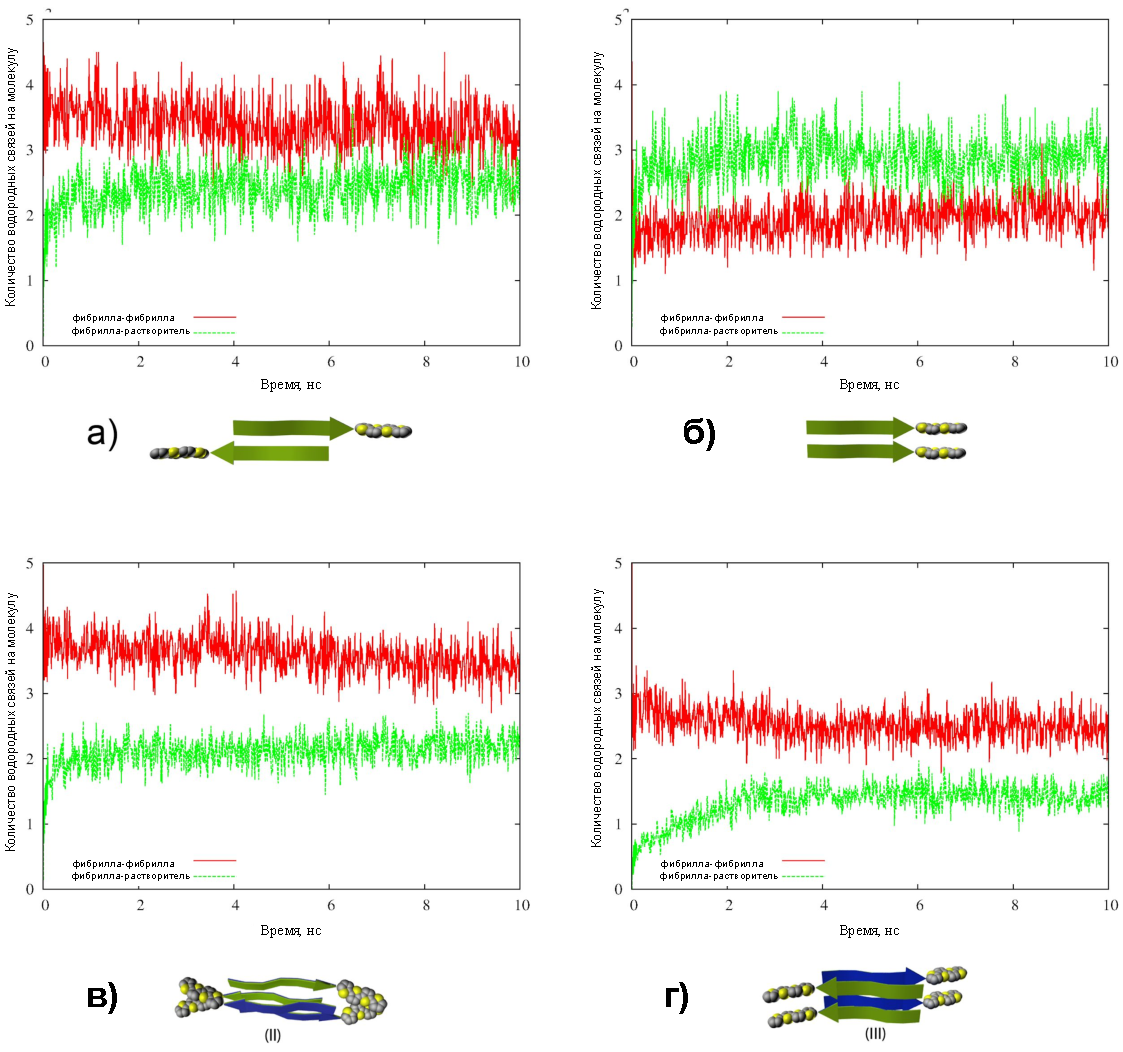
\includegraphics[width=\textwidth]{images/p4/punkt5/part4_p5_f38.pdf}
    \caption[Число водородных связей на одну гибридную молекулу как функция времени моделирования]{Число водородных связей на одну гибридную молекулу как функция времени моделирования.}
    \label{fig:p4_p5_f38}
\end{figure}


    \textbf{Упаковка пептидов}

    Для дальнейшего анализа конформации пептидных фрагментов в фибриллах был проведен анализ вторичной структуры пептидного остова, представленного на рисунке \ref{fig:p4_p5_f39}, с использованием алгоритма STRIDE \cite{frishman_knowledge-based_1995}. Выявлено высокое преобладание $\beta$-листовой структуры фибрилл на основе антипараллельного расположения (70\% для SL-AP и 75\% для DL-AP). Последовательность из пептидного хвоста гибридной молекулы, которая была проанализирована с помощью STRIDE, состоит из 11 аминокислот: GLY- [THR-VAL] 3-GLY-PHE-GLY и специально включенного $\beta$-листа, образующего $[THR-VAL]_3$ последовательность составляет только 55\% от общей последовательности. Таким образом, можно видеть, что для антипараллельного расположения склонность к $\beta$-слою выходит далеко за пределы последовательности $[THR-VAL]_3$ и включает также соседние аминокислотные остатки.

    Для параллельных расположений склонность формирования $\beta$-структуры составляла 45\% (+ 1\% $\beta$-мостов) для SL-PAR и 47\% (+ 4\% $\beta$-мостов) для фибрилл DL-PAR. Снова видно, что двухслойные укладки немного более упорядочены и имеют немного большую часть структуры в виде $\beta$-листов. Часть пептидной последовательности, которая организована в $\beta$-лист или $\beta$-мостики для параллельного расположения, значительно меньше, чем для антипараллельного, однако это соответствует общей менее точной структуре параллельных $\beta$-листов с точки зрения регулярности водородных связей. В любом случае для фибриллы DL-PAR совокупная склонность структуры к $\beta$-листам составляет 51\%, что очень близко к доле последовательности $[THR-VAL]_3$ в общей последовательности, и эту последовательность можно рассматривать как идеальный $\beta$-лист.

\begin{figure} [H]
    \centering
    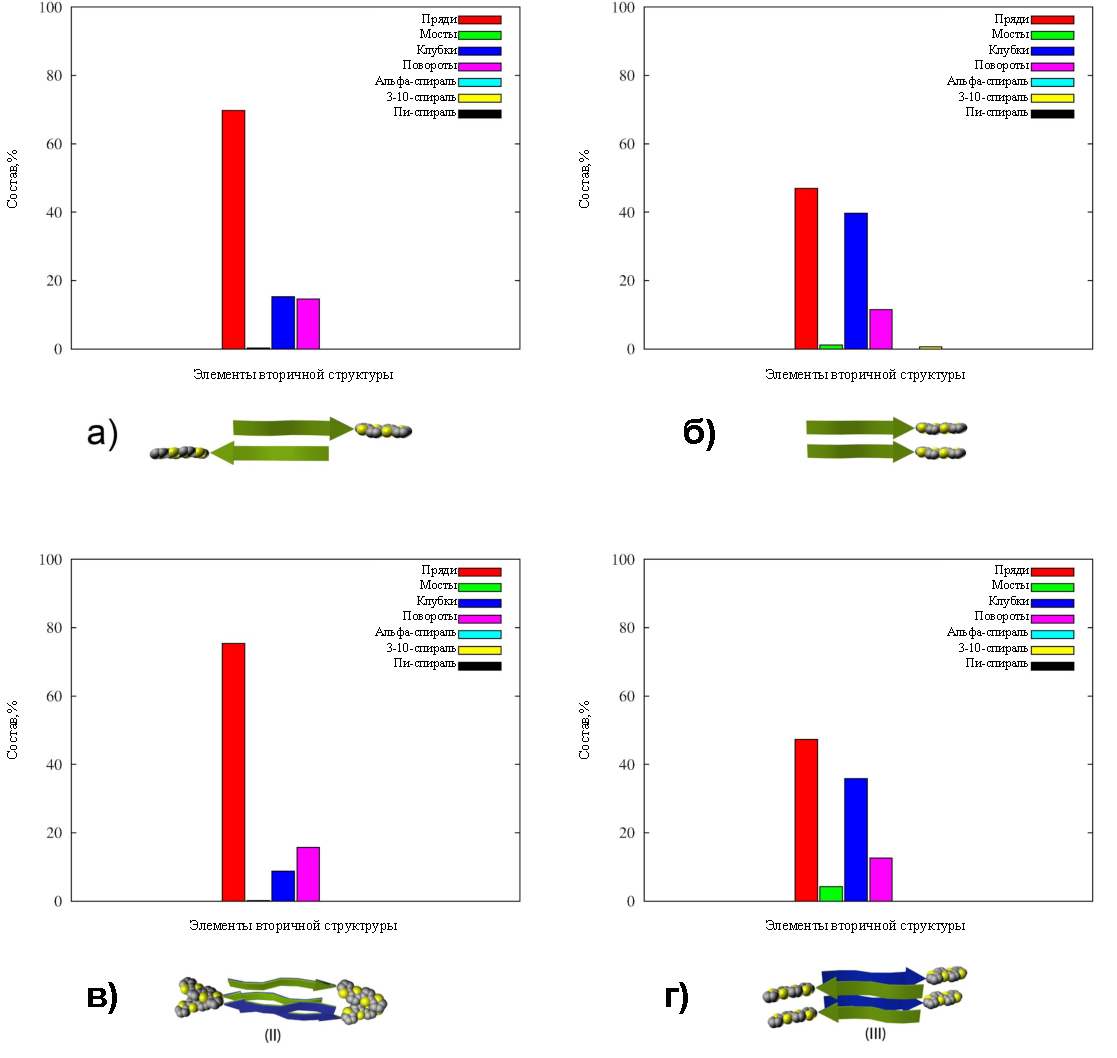
\includegraphics[width=\textwidth]{images/p4/punkt5/part4_p5_f39.pdf}
    \caption[Гистограммы элементов вторичной структуры в различных фибриллах, смоделированных в растворителе]{Гистограммы элементов вторичной структуры в различных фибриллах, смоделированных в растворителе. Данные усредняются за последние 2 нс моделирования. Фибриллы обозначены их пиктограммами под графиками: а) фибрилла SL-AP, б) фибрилла SL-PAR, в) фибрилла DL-AP, г) фибрилла DL-PAR.}
    \label{fig:p4_p5_f39}
\end{figure}

    Анализ расположения пептида и тиофена также проводился с помощью гистограмм линейного распределения расстояний между центрами масс пептидных и тиофеновых фрагментов (см. рис. \ref{fig:p4_p5_f40}). Эти графики ясно указывают на то, что пептидные фрагменты надежно организованы с хорошим дальним порядком. Сравнение графиков снова показывает, что укладки с двумя слоями имеют лучший дальний порядок, чем укладки с одним слоем. Координаты второго основного пика красных линий (распределения пептид-пептид) представляют периодичность структуры и читаются следующим образом: SL-AP - 0,95 нм, SL-PAR - 0,98 нм, DL-AP - 0,96 нм, DL- PAR - 1.0 нм, что при делении на 2 дает расстояние между нитями. Мы видим, что антипараллельное расположение имеет несколько более узкую упаковку $\beta$-нитей 4,8\AA{}  между пептидами по сравнению с 4,9-5,0\AA\  при параллельном расположении.

    Как видно из графиков, периодическое расположение пептидных фрагментов передается тиофеновым фрагментам в случае фибрилл SL-PAR, DL-PAR и DL-AP. Наилучший дальний порядок блоков кватротиофена достигается для фибриллы DL-PAR, тогда как в случае SL-AP упорядочение почти не наблюдается.

    Пики гистограмм распределения тиофен-тиофена повторяют пики гистограмм пептид-пептид, но не в точности. Для параллельных расположений первый пик для тиофеновых фрагментов находится при 0,54 нм как для SL-PAR, так и для DL-PAR. Этот сдвиг межтиофенового расстояния по сравнению с межпептидным расстоянием можно объяснить только осевым скручиванием фибриллы. Хотя фибрилла SL-PAR является более динамичной, и ее поведение при осевом скручивании нельзя сразу увидеть при визуальном осмотре (из-за скручивания фибриллы), соответствие ее функции распределения функции DL-PAR четко указывает на то, что скручивание  - это внутреннее свойство уже однослойной фибриллы.

    Для фибриллы DL-AP первый и второй пики распределения тиофен-тиофен соответствуют 0,57 и 0,86 нм, что можно объяснить латеральным сдвигом тиофеновых фрагментов по отношению друг к другу, поскольку этот тип структуры менее регулярен и прост, чем тот, который основан на параллельном расположении.



\begin{figure} [H]
    \centering
    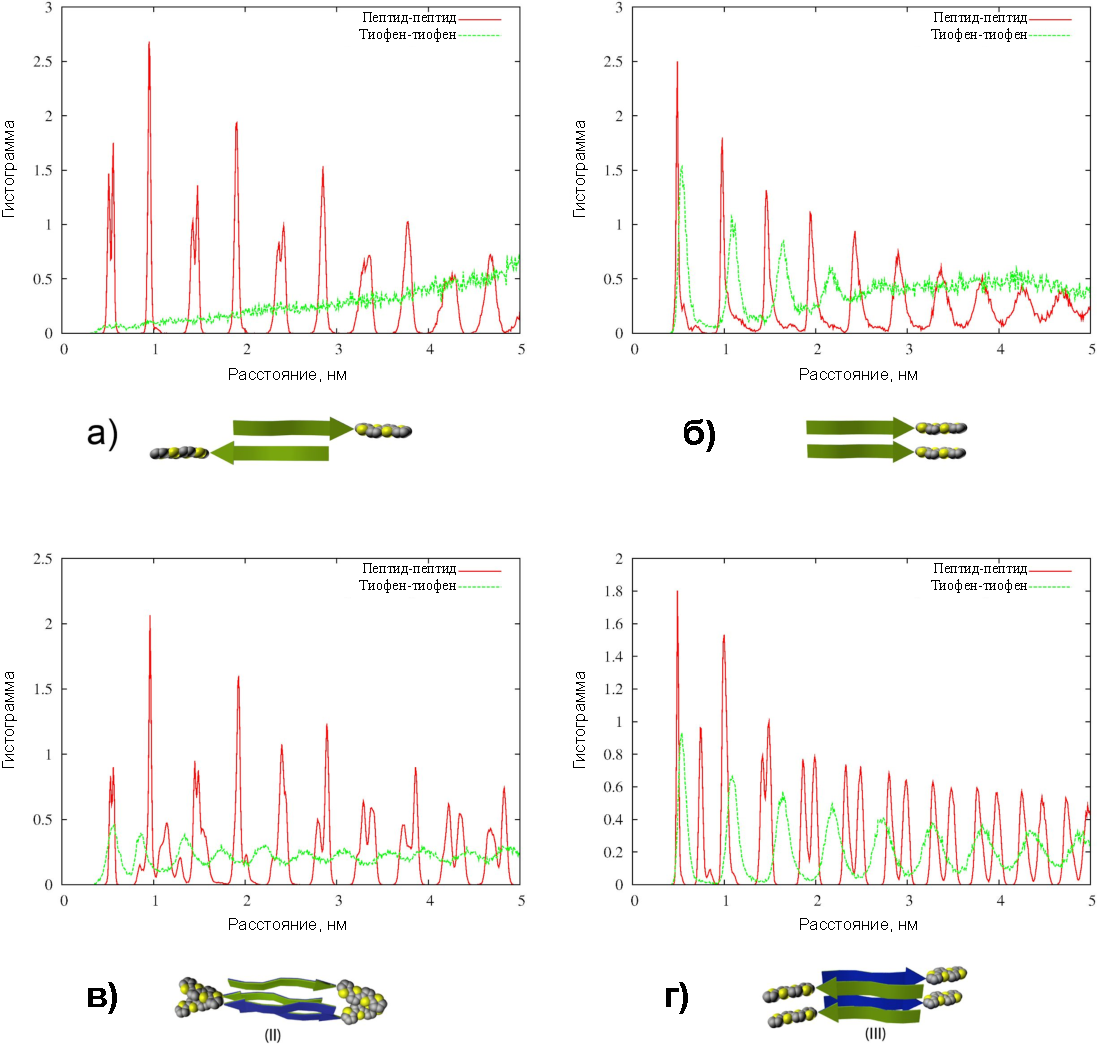
\includegraphics[width=\textwidth]{images/p4/punkt5/part4_p5_f40.pdf}
    \caption[Линейное распределение пептидных и тиофеновых блоков в фибриллах]{Линейное распределение пептидных и тиофеновых блоков в фибриллах. Все расстояния были рассчитаны между центрами масс блоков $[THR-VAL]_3$ или блоков кватротиофена за последние 2 нс траектории моделирования. Распределения нормированы на (10 - x), где x - расстояние.}
    \label{fig:p4_p5_f40}
\end{figure}


    \emph{\textbf{Упаковка тиофена}}

    Теперь мы можем приступить к анализу упорядочения тиофенов в наших фибриллах - вопрос, который имеет первостепенный интерес с точки зрения возможного применения фибрилл в области органической электроники.
    
    Сначала приступим к качественному описанию. Увеличенные снимки упорядочения блоков кватротиофена представлены на рисунке \ref{fig:p4_p5_f41}.

    \emph{Качественное описание.}
    
    В фибрилле SL-AP (как видно во время моделирования и как видно из снимка на рис. \ref{fig:p4_p5_f41}a) блоки кватротиофена очень конформационно подвижны. Поскольку тиофены сами по себе являются жесткими, их конформационная подвижность частично обусловлена подвижностью боковой цепи пара-азидофенилаланинового линкера, через которую соединен тиофеновый блок, и частично (ii) вращением двугранного угла между фенилаланином и глицином, образуя своего рода глициновый шарнир. Последний тип конформационной подвижности может приводить к значительно различающимся ориентациям тиофеновой составляющей, как видно на рисунке \ref{fig:p4_p5_f41}а, некоторые тиофеновые блоки могут даже указывать в противоположном направлении по сравнению с другими блоками. Эта чрезвычайная гибкость также обеспечивается тем фактом, что в этом типе фибрилл тиофены расположены на расстоянии двух $\beta$-нитей ($\sim 1$нм) друг от друга, что фактически не оставляет возможности для взаимодействия и переноса электронов.

    Структура тиофена в фибриллах SL-PAR (рис. \ref{fig:p4_p5_f41}б) более устойчива, поскольку тиофены здесь расположены ближе в пределах одинарного $\beta$-цепочечного расстояния ($\sim 0,5$ нм) и имеют возможность стерически взаимодействовать. Это стерическое взаимодействие, однако, недостаточно сильное, чтобы удерживать вместе все тиофеновые фрагменты, они поворачиваются, чтобы сформировать области плотной упаковки, разделенные промежутками, и эта структура все еще динамична - промежутки имеют тенденцию закрываться и появляться снова. Появлению зазоров также способствует несоответствие расстояний упаковки: для тиофенов идеальное расстояние для укладки $\pi - \pi$ составляет около 3,3-3,5\AA{} \cite{rodriguez-ropero_ab_2008,tsuzuki_model_2002}, в то время как расстояние между $\beta$-нитями составляет около 5\AA, поэтому тиофены должны приспосабливаться к расстоянию, обеспечиваемому $\beta$-листом, либо за счет образования промежутков, либо за счет наклона.

    Двухслойные тиофены образуют более упорядоченную структуру; однако фибрилла DL-AP все еще не имеет степени упорядочения, необходимой для хорошего переноса электронов. Как видно на рисунке \ref{fig:p4_p5_f41}в, из-за несоответствия расстояния тиофены слипаются, но имеют промежутки между непрерывными стопками тиофенов (верхний ряд), или из-за гибкости линкерных аминокислот тиофены могут изменять свою ориентацию, вращаться так, чтобы их плоскости были выровнены вдоль фибрилл (см. нижний ряд), так что не образуется непрерывная тиофеновая стопка, способная переносить электроны вдоль фибриллы. Кроме того, в этой фибрилле тиофены не идеально расположены латерально для стэкинг взаимодействия.

    Фибрилла DL-PAR, по-видимому, содержит тиофены в лучшем порядке среди изученных, тиофены расположены в однородном порядке с некоторым изгибом и наклоном вдоль оси фибриллы (см. Рисунок \ref{fig:p4_p5_f41}г). Тиофены находятся в динамическом порядке - могут образовываться щели между соседними тиофенами в стопке, но они ``заживают'' за десятки пикосекунд.


\begin{figure} [H]
    \centering
    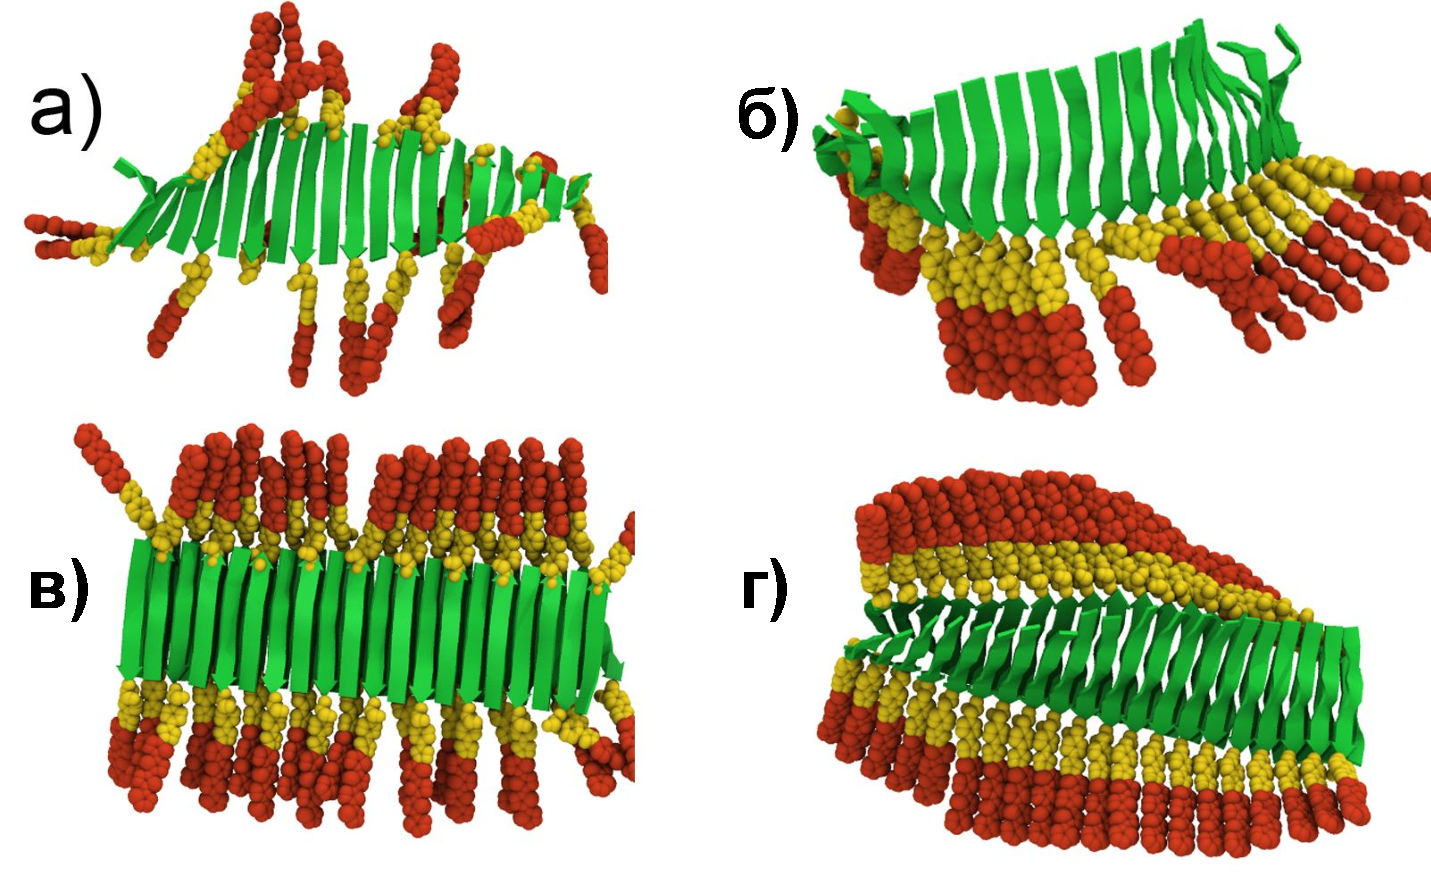
\includegraphics[width=\textwidth]{images/p4/punkt5/part4_p5_f41.pdf}
    \caption{Снимки расположения блоков кватротиофена в моделируемых фибриллах различных типов: а) фибрилла SL-AP, б) фибрилла SL-PAR, в) фибрилла DL-AP, г) фибрилла DL-PAR. Алкильные цепи не изображены для ясности представления.}
    \label{fig:p4_p5_f41}
\end{figure}

    \emph{Количественное описание}

    Качественно описав упорядочение тиофена в различных типах фибрилл, мы теперь количественно опишем положение соседних тиофеновых фрагментов с точки зрения их порядка, расстояния и ориентации. Для этого мы определяем три основных вектора, связанных с каждым блоком кватротиофена, вектор TI1-TI4, вектор нормали к поверхности и третий дополнительный вектор (см. Рисунок \ref{fig:p4_p5_f42}a). Вектор TI1-TI4 - это вектор, соединяющий центры масс первого и последнего тиофенового кольца в кватротиофене, вектор нормали к поверхности можно рассматривать как вектор, представляющий среднюю плоскость фрагмента кватротиофена, вычисленную как среднее из векторов нормалей каждого тиофенового кольца. Дополнительный вектор перпендикулярен двум векторам. Эти три вектора позже будут обозначаться как x, y и z, как показано на рисунке \ref{fig:p4_p5_f42}a.

    С точки зрения этих векторов, их упорядочения и положения соседних тиофеновых фрагментов по отношению к этим векторам было проанализировано упорядочение блоков кватротиофена, данные представлены в Таблице \ref{tab:p4_t2} и рисунке \ref{fig:p4_p5_f42}.

%TABLE2-----------------------------------------
\begin{table}[H]
    \centering
    \begin{tabularx}{\textwidth}{X|X|X|X|X|X|X}
        Тип фибриллы & Наиболее вероятное расстояние,\AA{} & Параметр порядка TI1-TI4 & Параметр порядка относительно нормали  к  поверхности & Среднее смещение x,\AA{} & Среднее смещение y,\AA{} & Среднее смещение z,\AA{} \\
        SL-PAR & 5.4 & 0.97 & 0.94 & 1.4 & 3.7 & 3.46 \\   
        DL-AP  & 5.7 & 0.82 & 0.96 & 2.9 & 2.4 & 3.47 \\
        DL-PAR & 5.4 & 0.98 & 0.95 & 2.0 & 3.3 & 3.55  
    \end{tabularx}
    \caption{Параметры порядка соседних блоков кватротиофена в фибриллах, рассчитанные в течение последних 2 нс моделирования.}
    \label{tab:p4_t2}
\end{table}

    Таблица \ref{tab:p4_t2} включает информацию о наиболее вероятном расстоянии между центрами масс соседних блоков кватротиофена, параметрах порядка (рассчитанных как$\big \langle P_2(\cos \vartheta )   \big \rangle$, где $P_2$ - второй полином Лежандра) для двух векторов и проекциях среднего расстояния между центрами масс тиофена на главные векторы (называемое средним смещением). Параметры среднего смещения позволяют охарактеризовать, как следующий кватротиофен в стопке расположен относительно предыдущего.

    Из таблицы можно увидеть, что укладки, основанные на параллельных $\beta$-листах, имеют более высокие параметры упорядочения тиофенов по сравнению с таковыми для фибриллы DL-AP для длинной оси тиофена (вектор TI1-TI4) (0,98 против 0,82). Однако параметр порядка для вектора нормали к поверхности, который описывает планарность соседних тиофенов, находится в сопоставимом масштабе (фактически даже лучше) для фибриллы DL-AP, чем для фибриллы DL-PAR.

    Гистограммы на рисунке \ref{fig:p4_p5_f42} дают дополнительную информацию об этом порядке тиофеновых фрагментов в фибриллах. Для SL-PAR и DL-AP угловые распределения для обоих векторов представляют собой узкие гауссовы пики в диапазоне от $0^{\circ}$ до $10^{\circ}$, тогда как для DL-AP ситуация иная. Для вектора TI1-TI4 максимум распределения составляет около $15^{\circ}$ и охватывает более широкую область от $0^{\circ}$ до $35^{\circ}$. Это указывает на то, что в направлении тиофенов все еще существует некоторый порядок, но они, как правило, не коллинеарны, а скорее имеют некоторый угол между собой. Для вектора нормали к поверхности ситуация немного иная: из-за структуры расположения смежные блоки кватротиофена имеют тенденцию быть антипараллельными по отношению к нормали к поверхности. Хотя распределение вектора нормали к поверхности в DL-AP имеет очень выраженный пик около $170^{\circ}$, что указывает на высокую компланарность тиофенов в этом типе фибрилл.

    Параметры смещения в таблице позволяют понять типичную конфигурацию тиофеновых фрагментов. Из последнего столбца видно, что среднее расстояние между плоскостями тиофенов составляет около 3,45–3,55\AA{}, что является верхним пределом идеального расстояния $\pi - \pi$-стэкинга  в 3,3–3,5\AA{} \cite{rodriguez-ropero_ab_2008,tsuzuki_model_2002}. Остальные значения дают ключ к пониманию кадров на рисунке \ref{fig:p4_p5_f41}.

\begin{figure} [H]
    \centering
    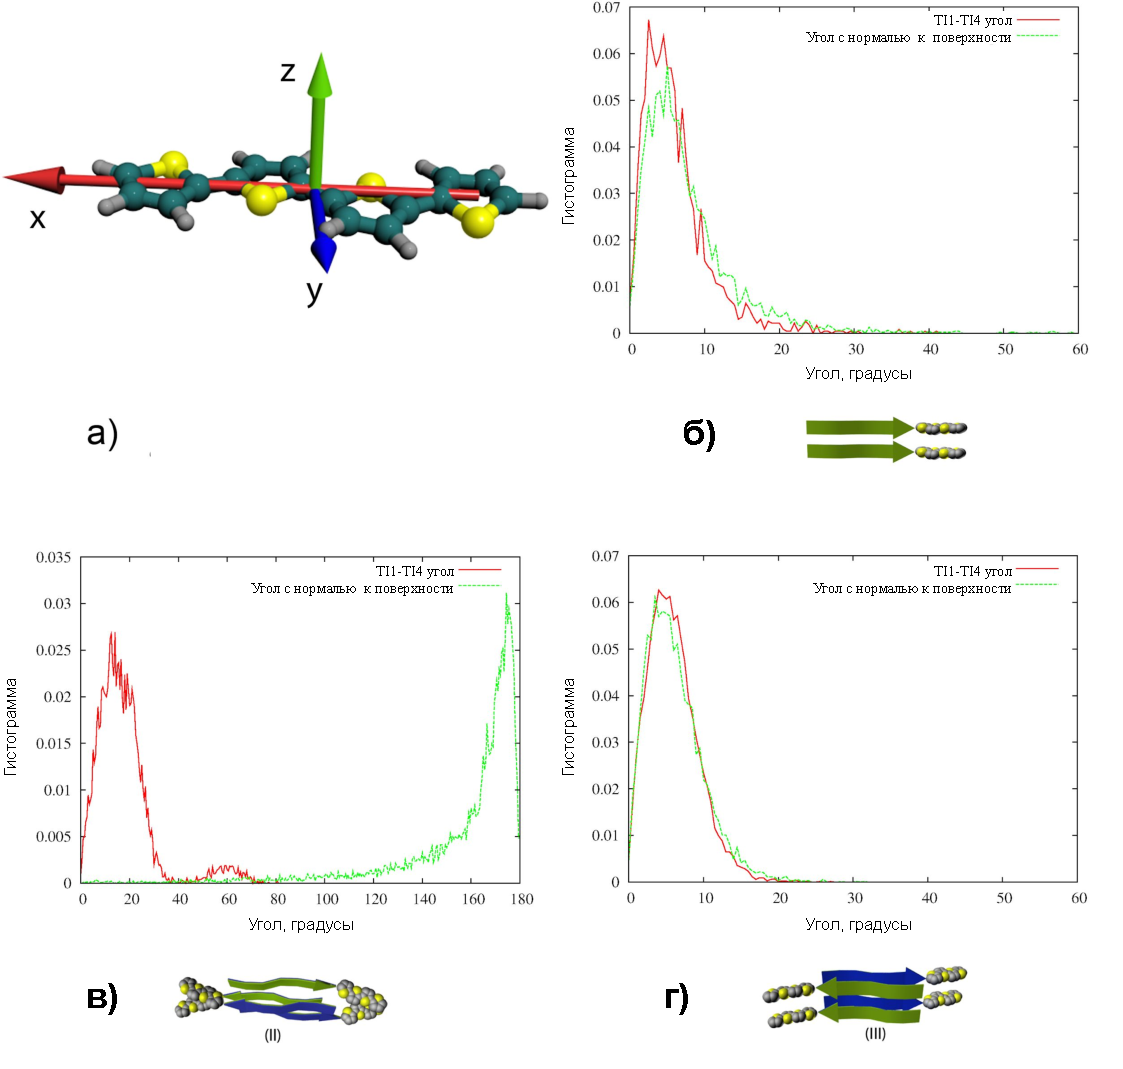
\includegraphics[width=\textwidth]{images/p4/punkt5/part4_p5_f42.pdf}
    \caption[Анализ упорядочения тиофенов в фибриллах]{Анализ упорядочения тиофенов в фибриллах. а) Графическое представление основных векторов в блоке кватротиофена, используемое для дальнейшего анализа упорядочения: красным - вектор, соединяющий центры масс первого и последнего тиофенового кольца (вектор TI1-TI4), зеленым - вектор, перпендикулярный среднему Плоскость поверхности тиофенового блока, синий - вектор, перпендикулярный двум другим векторам. б), в), г) гистограммы угловых распределений между TI1-TI4 и векторами нормали к поверхности соседних блоков кватротиофена для фибрилл SL-PAR, DL-AP и DL-PAR соответственно.}
    \label{fig:p4_p5_f42}
\end{figure}


\subsubsection{Методы и детали}

    \emph{\textbf{Методы моделирования}}

    Моделирование фибрилл в растворителе проводилось в пакете моделирования LAMMPS \cite{plimpton_fast_1995}. Моделирование проводилось со следующими параметрами: взаимодействие Ленарда-Джонса, радиус обрезания 10\AA, электростатические взаимодействия обрабатывались с помощью алгоритма PPPM \cite{hockney_computer_1989} с реальным пространственным отсечением 10\AA{} и значением точности $10^{-4}$, динамика Ланжевена с $T=300 K$ и параметром демпфирования 0,5 $пс^{-1}$, был применен алгоритм поддержания изотропного давления Берендсена с эталонным давлением 1 атм, параметром времени демпфирования 2 пс и объемным модулем сжатия системы в 20000 атм, что находится в диапазоне модуля объемной упругости типичных жидкостей. Шаг интегрирования для первых 100 пс моделирования составлял 0,1 фс, чтобы обеспечить плавную релаксацию для системы, в то время как для остальной части моделирования он составлял 1 фс.

    Моделирование проводилось параллельно с использованием техники декомпозиции доменов на 512 процессорах одновременно.

    \emph{\textbf{Методы анализа}}

    Визуализация была выполнена с помощью программы VMD \cite{humphrey_vmd_1996} и трассировщика лучей Tachyon \cite{stone_efficient_1998}.

    Водородные связи определяли с использованием модуля VMD. Считалось, что водородная связь образуется между атомом с присоединенным к нему водородом (донор, D) и другим атомом (акцептор, A) при условии, что расстояние DA меньше, чем расстояние отсечки 3,0\AA{} и угол DHA меньше предельного угла 20 градусов.

    Для определения вторичной структуры использовался алгоритм STRIDE \cite{frishman_knowledge-based_1995}.

    Для анализа тиофена были рассмотрены тиофены с расстояниями между ними менее 6\AA. Основные векторы были рассчитаны следующим образом: вектор TI1-TI4 (x-вектор) - это вектор, соединяющий центры масс первого и последнего тиофенового кольца в кватротиофеновом блоке. В качестве предварительного шага для вычисления y-вектора были вычислены векторы, связывающие центр масс атомов углерода с атомом серы для каждого тиофенового кольца. Комбинация этих четырех векторов с чередующимися знаками определила y-вектор. Затем вычисляли вектор нормали к поверхности (z-вектор) как векторное произведение x-вектора и y-вектора. Анализ проводился на основе последних 2 нс моделирования.


\subsection{Крупномасштабное моделирование морфологии агрегатов в вакууме}

    Наша следующая цель в многомасштабном моделировании - изучить крупномасштабную конформационную морфологию фибрилл на основе выбранных молекулярных расположений в масштабе длины, сравнимом с теми, которые могут быть зафиксированы измерениями АСМ и ПЭМ (обычно десятки нанометров), таким образом, чтобы стало возможным некоторое сравнение между экспериментальными результатами и результатами моделирования.
    
    К сожалению, моделирование длинных фибрилл в явном растворителе сейчас кажется недостижимой целью, поскольку (i) размер системы требует больших вычислительных ресурсов, (ii) время эволюции, необходимое для того, чтобы большая система приняла свою отрелаксированную конформацию, составляет намного дольше, и растворитель предотвращает крупномасштабные конформационные переходы за разумное время моделирования.
    
    В этой работе мы решили опустить явные молекулы растворителя, но все же частично имитировать растворитель, используя подход диссипативной динамики частиц.

    Как и в предыдущем разделе, две однослойных периодических укладки и две двухслойных укладки использовались для создания длинных фибрилл путем репликации периодической ячейки вдоль оси филамента. Для выбранных систем были сконструированы плоские прямые фибриллы с длиной 80 $\beta$-нитей (приблизительно 40 нм) и подвергнуты моделированию методом МД до 10 нс с использованием термостата на основе метода диссипативной динамики частиц со специальным протоколом релаксации и нагрева (см. Подраздел ``Методы''), использованного в течение первых 2,5. нс моделирования. Длина фибриллярных агрегатов была выбрана достаточно большой, чтобы избежать влияния возможных ``краевых'' эффектов на общую конформацию агрегатов (которая для амилоидных фибрилл родственного происхождения может быть оценена в 10 нм \cite{xu_alzheimers_2010}) с одной стороны, и вычислительная сложность задачи была разумной с другой стороны. Длина фибриллярных агрегатов, используемых в современных работах по полноатомному моделированию амилоидных фибрилл, что, как считается, позволяет проследить их геометрические характеристики, составляет около 20-30 нм \cite{paparcone_atomistic_2010,paparcone_microscale_2009}.

    Исходные структуры фибрилл и их эволюцию во время моделирования можно увидеть на рисунках \ref{fig:p4_p5_f43} и \ref{fig:p4_p5_f44}. Большие конформационные изменения, которые происходят в течение короткого времени моделирования, были одной из методологических проблем настоящей работы, другой проблемой был правильный учет дальних взаимодействий, поскольку оказалось, что дальнодействующие взаимодействия (такие как электростатические взаимодействия) ответственны за крупномасштабное конформационное поведение фибрилл, и их усечение на малых расстояниях может изменить крупномасштабную конформацию фибрилл. Эти вопросы дополнительно разъясняются в следующем разделе о методах.

    Чтобы изучить влияние тиофеновой и пептидной составляющих на крупномасштабную морфологию фибрилл, мы дополнительно провели моделирование фибрилл, состоящих только из пептидной части гибридных молекул (см. рисунок \ref{fig:p4_p5_f45}).

\subsubsection{Результаты}

    \emph{\textbf{Качественное описание}}

    Значительное увеличение длины агрегатов фибрилл по сравнению с предыдущим исследованием позволило выявить морфологию агрегатов и их поведение в более крупном нанометровом масштабе в режиме, когда длина фибрилл намного больше их ширины.

    Конформационная эволюция сконструированных агрегатов во время моделирования позволяет как изучить форму и морфологию фибрилл, так и проследить влияние межмолекулярного расположения на конформацию агрегатов на наномасштабе. Сравнительный анализ различных фибрилл позволяет обсудить роль различных межмолекулярных взаимодействий в стабильности и поведении агрегатов.

    Исчерпывающий список моментальных снимков, описывающих конформационную эволюцию различных типов фибрилл, представлен на рисунках \ref{fig:p4_p5_f43} и \ref{fig:p4_p5_f44}. Хотя все системы продемонстрировали свою стабильность в ходе моделирования, то есть все молекулы сохранили свое относительное положение в агрегатах относительно их соседей, наблюдались конформационные перестройки как на молекулярном, так и на надмолекулярном уровне. Во всех случаях организация $\beta$-листов доминировала в структуре и оставалась основным каркасом для организации фибрилл. Протокола релаксации в 2,5 нс в сочетании с дальнейшим моделированием в течение 1-7 нс было достаточно, чтобы понять основные характеристики морфологии фибрилл и ее эволюцию (изгиб, кручение, закручивание и т. д.).
    
    Как видно из рисунка \ref{fig:p4_p5_f43}, однослойные фибриллы способны к более выраженной конформационной перестройке, чем двухслойные фибриллы, поскольку двухслойная организация фибрилл делает их жесткими.

    Моделирование длинных однослойных фибрилл (рис. \ref{fig:p4_p5_f43}) показывает различные типы конформационной морфологии скручивания, которые могут принимать фибриллы. Фибрилла SL-AP (рис. \ref{fig:p4_p5_f43}а) изменила свою конформацию таким образом, что лист начал завиваться, образуя тип плотно намотанной ленты с левосторонней спиралью с шагом спирали около 10 нм и углом спирали около $30^{\circ}$. Фибрилла SL-PAR (рис. \ref{fig:p4_p5_f43}б) образовывала другой тип ленты с левосторонней спиралью, ее шаг спирали составляет около 7 нм, а угол спирали близок к $90^{\circ}$, образуя таким образом полую кольцеобразную структуру.
    
    По геометрическим соображениям левая осевая скрученная лента ($\beta$-лист) скручивается, образуя левую спираль из этой ленты, однако эта спираль может иметь два разных типа, если поверхности ленты ($\beta$-лист ) разные (в нашем случае гидрофобные или гидрофильные). Легко показать, что эти два типа отличаются поверхностью ленты, которая обращена на внутреннюю или внешнюю сторону спирали. Эффекты растворителя должны играть значительную роль в скручивании спирали, и это должно зависеть от баланса между взаимодействиями боковых цепей на каждой стороне ленты друг с другом, а также с растворителем. В ранее проведенном моделировании коротких фибрилл в растворителе указывает на тип скручивания, когда боковые цепи треонина (гидрофильная сторона ленты) находятся на внутренней стороне спирали, однако эти фибриллы были недостаточно длинными. чтобы выявить этот эффект в более широком масштабе. Моделирование длинных фибрилл в вакууме действительно подтвердило это наблюдение: фибриллы SL-AP и SL-PAR закручены в спираль таким образом, что боковые цепи треонина находились внутри спирали. Предпочтение фибрилл скручиваться таким образом можно объяснить тем фактом, что во время скручивания боковые цепи треонина сближаются и образуют дополнительные водородные, что является энергетически выгодным. Для моделирования чистых пептидных фибрилл (см. рисунок \ref{fig:p4_p5_f45}) наблюдали такое же поведение, таким образом, этот тип скручивания является характерной особенностью пептидного остова фибриллы и на него не влияют взаимодействия тиофена или алкильной цепи.
    
    Однако следует отметить, что моделирование в вакууме играет вспомогательную роль в выявлении геометрии изгибающихся фибрилл, а не как средство определения точного параметра их геометрии, поскольку отсутствие растворителя не только перенормирует взаимодействия, но и делает конформационный энергетический ландшафт довольно неровным, начальная планарная конформация фибриллы энергетически очень неблагоприятна и нестабильна. Что касается типа завивки (гидрофильная или гидрофобная сердцевина спирали), моделирование с растворителем следует рассматривать как более надежное свидетельство типа завивки. Так, в нашей более ранней работе \cite{shaytan_self-organizing_2011} было, например, замечено, что при несколько иных условиях фибрилла SL-AP в вакууме эволюционировала в спираль с гидрофобным ядром, в то время как чистая пептидная фибрилла все еще завивалась в спираль с гидрофильным ядром.

    В отличие от однослойных фибрилл, двухслойные фибриллы дают гораздо более жесткие и линейные ленты из фибрилл. Фибрилла DL-AP (рис. \ref{fig:p4_p5_f44}а) превратилась в слегка скрученную влево ленту, которая изгибается примерно на $30^{\circ}$ на 80 $\beta$-нитей. В течение начального периода релаксации (см. График расстояний от конца до конца на Рисунке \ref{fig:p4_p5_f44}a) фибрилла испытывает высокие конформационные изгибные флуктуации с изменением направления изгиба, поскольку избыточная кинетическая энергия отводится от фибриллы, она принимает стабильную изогнутую форму с некоторыми колебаниями вокруг него. Общее осевое скручивание можно оценить примерно в $1^{\circ}$ на $\beta$-нить.
    
 
    Фибрилла DL-PAR (рис. \ref{fig:p4_p5_f44}а) проявляет несколько иной тип поведения; она приняла значительно более закрученную в осевом направлении конформацию с приблизительно $2,8^{\circ}$ на $\beta$-нити, в то время как почти не наблюдалось предпочтительного изгиба фибриллы. Сравнивая поведение фибрилл DL-AP и DL-PAR, можно дополнительно предположить, что повышенная скорость скручивания приводит к увеличению жесткости фибриллы на изгиб. Более того, из соображений симметрии весьма вероятно, что наблюдаемому изгибу фибриллы DL-AP частично способствуют эффекты конечного размера, поскольку длины фибриллы недостаточно, чтобы проявить полное влияние аксиального скручивания (когда фибрилла закручивается не менее чем на $180^{\circ}$), в то время как скручивание делает фибриллу осесимметричной и, таким образом, предпочтительное направление изгиба может быть потеряно. Следовательно, вероятно, что в еще большем масштабе морфологические различия DL-AP и DL-PAR фибрилл будут редуцированы только до различного периода осевого скручивания и персистентной длины. Наши текущие данные моделирования предсказывают приблизительное значение расстояния спиральной закрутки (когда плоскость фибриллярной ленты закручена на $360^{\circ}$) для DL-AP - 170 нм, для DL-PAR около 60 нм. 


    Стоит также сравнить моделирование тиофен-пептидных фибрилл и чистых пептидных фибрилл (см. рисунок \ref{fig:p4_p5_f45}). Из снимков видно, что основная конформационная структура одинакова, т.е. пептидный остов играет доминирующую роль в определении общей конформации. Однако видны определенные различия, которые можно объяснить влиянием блоков алкилированного кватротиофена: (i) фибрилла SL-AP становится более компактной в присутствии синтетических блоков, (ii) для фибриллы SL-PAR присутствие синтетических блоков препятствует взаимодействию конца фибриллы и делает структуру менее узловатой, (iii) для фибриллы чистого пептида DL-AP не наблюдалось предпочтительного изгиба, что означает, что синтетические блоки могут вызывать дополнительное изгибание фибриллы для насыщения их стерических взаимодействий.


\begin{figure} [H]
    \centering
    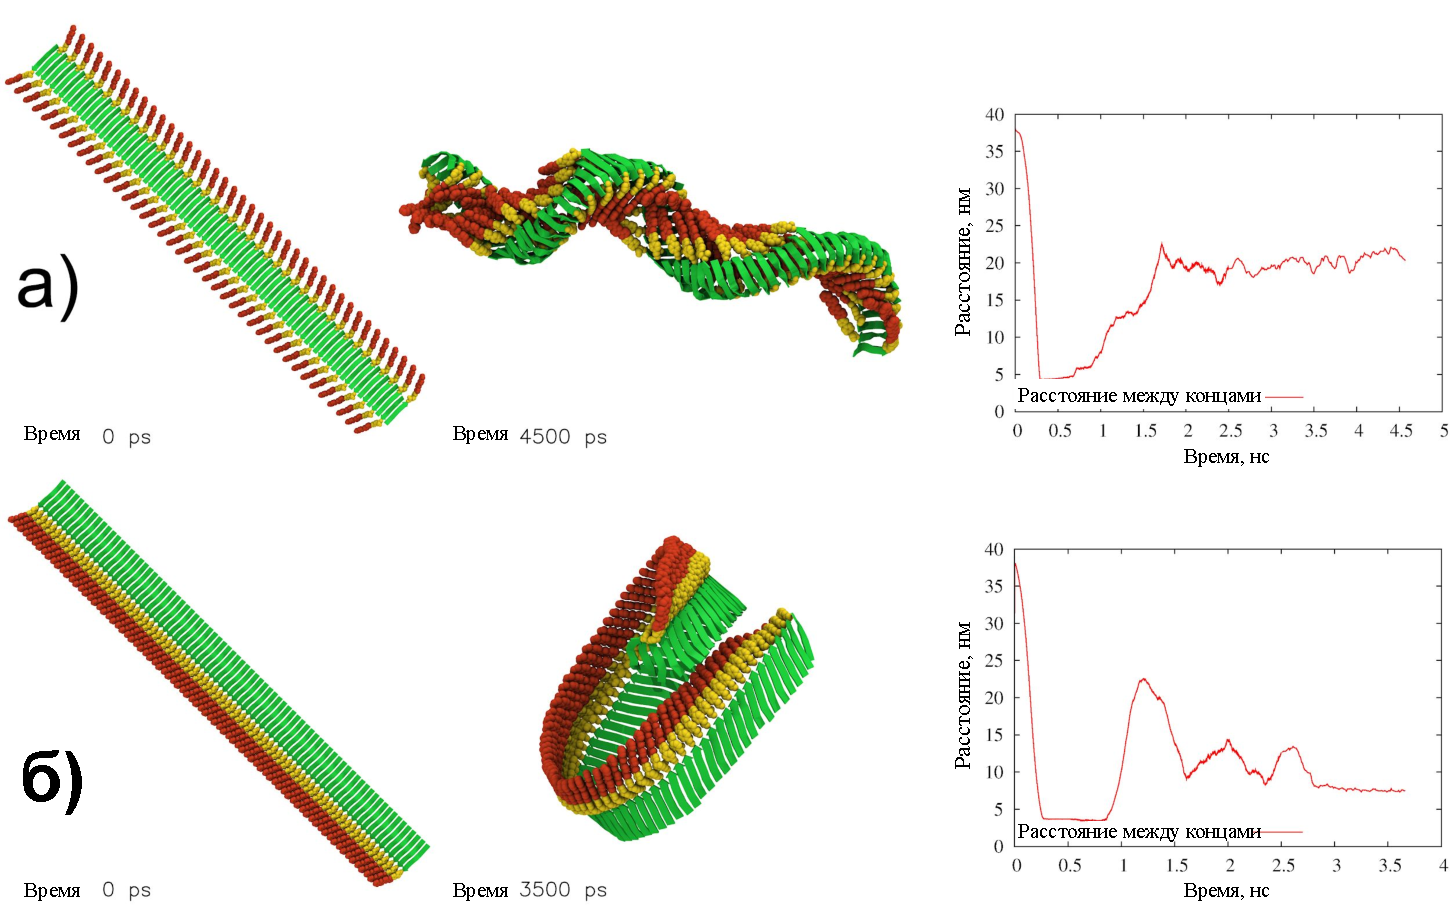
\includegraphics[width=\textwidth]{images/p4/punkt5/part4_p5_f43.pdf}
    \caption[Первоначальные снимки и эволюция фибрилл во время моделирования однослойных структур тиофен-пептид]{Первоначальные снимки и эволюция фибрилл во время моделирования однослойных структур тиофен-пептид, а также график эволюции расстояния от конца до конца: а) фибрилла типа SL-AP, б) фибрилла типа SL-PAR. Алкильные хвосты не изображены, тиофеновая часть изображена красными сферами, пара-азидофенилаланиновый линкер изображен желтым цветом, пептидные части изображены зелеными стрелками.}
    \label{fig:p4_p5_f43}
\end{figure}


\begin{figure} [H]
    \centering
    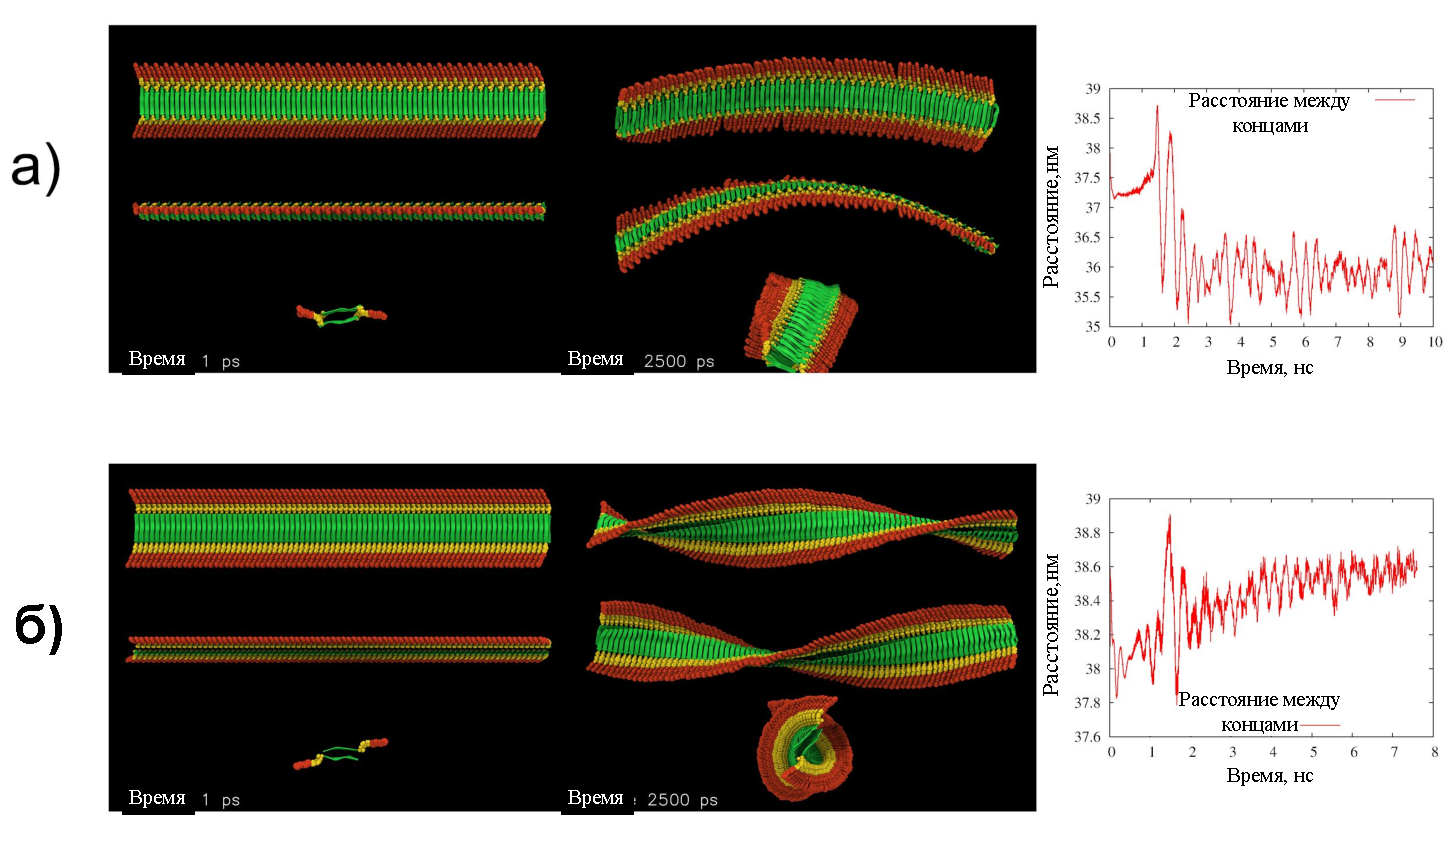
\includegraphics[width=\textwidth]{images/p4/punkt5/part4_p5_f44.pdf}
    \caption[Первоначальные снимки и эволюция фибрилл во время моделирования двухслойных структур тиофен-пептид]{Первоначальные снимки и эволюция фибрилл во время моделирования двухслойных структур тиофен-пептид, а также график эволюции расстояния от конца до конца: а) фибрилла типа DL-AP, б) фибрилла типа DL-PAR. Одна и та же фибрилла изображена в трех проекциях. Алкильные хвосты не изображены, тиофеновая часть изображена красными сферами, пара-азидофенилаланиновый линкер изображен желтым цветом, пептидные части изображены зелеными стрелками.}
    \label{fig:p4_p5_f44}
\end{figure}


\begin{figure} [H]
    \centering
    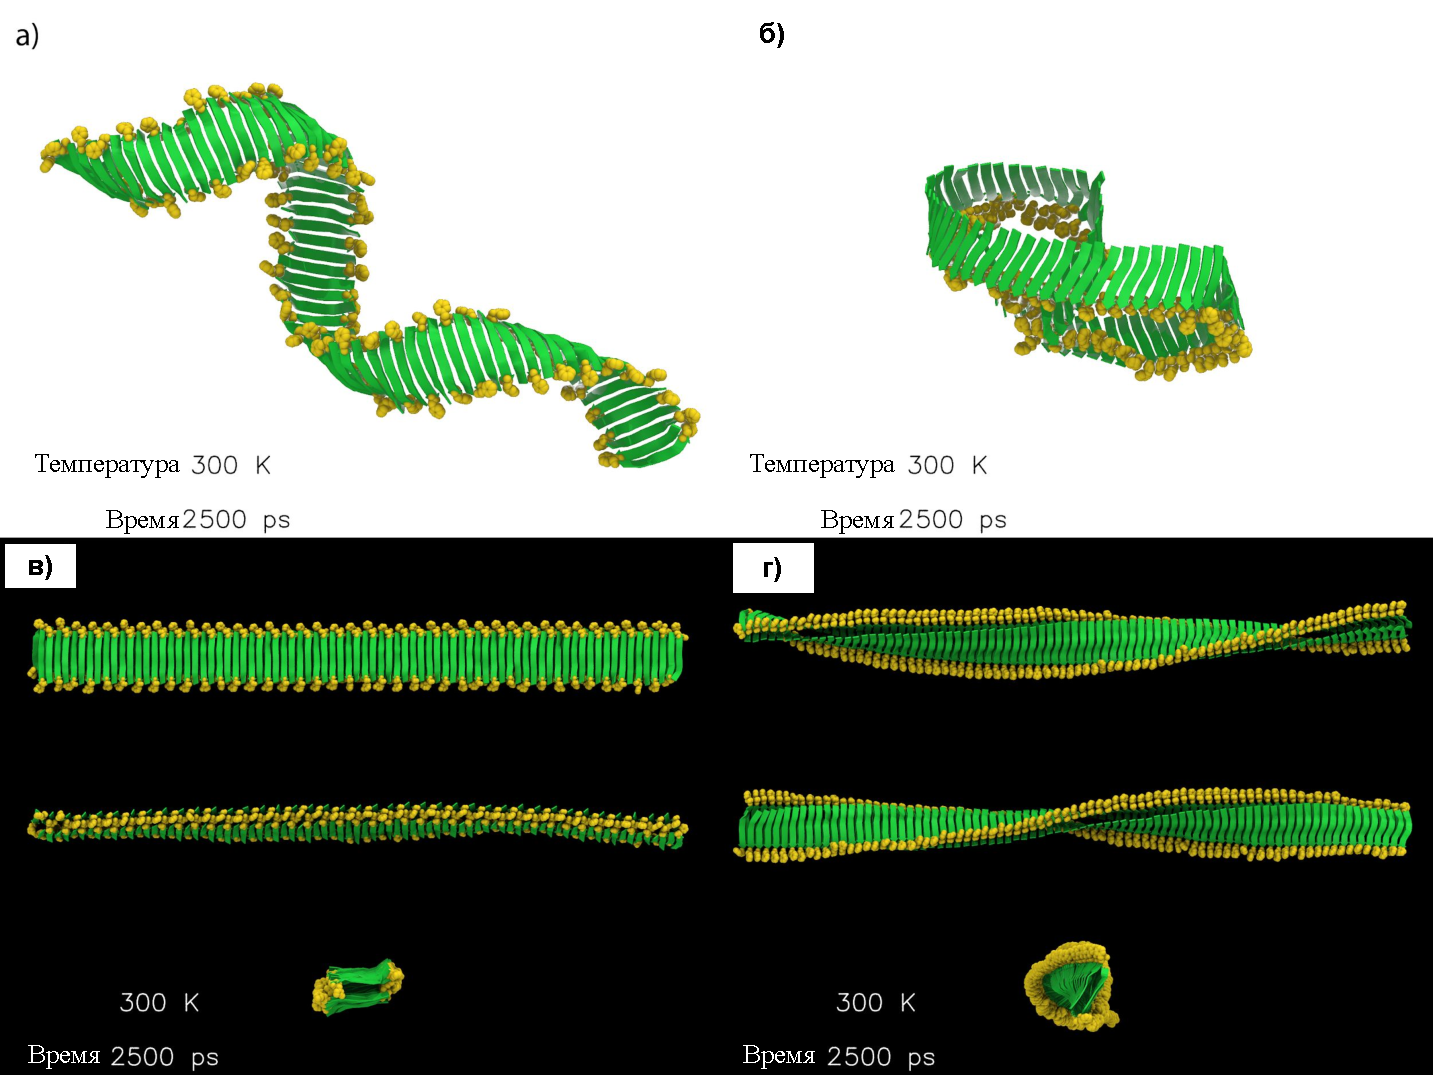
\includegraphics[width=\textwidth]{images/p4/punkt5/part4_p5_f45.pdf}
    \caption[Снимки окончательной конформации чистых пептидных фибрилл (без кватротиофеновых фрагментов)]{Снимки окончательной конформации чистых пептидных фибрилл (без кватротиофеновых фрагментов). Пептидный остов изображен зелеными стрелками, боковая цепь фенилаланина, которая ранее использовалась для соединения тиофена, изображена желтым. Пептидные фибриллы соответствуют следующим гибридным фибриллам: SL-AP (a), SL-PAR (б), DL-AP (в), DL-PAR (г).}
    \label{fig:p4_p5_f45}
\end{figure}


    \emph{\textbf{Количественное описание}}

    Характерные геометрические параметры окончательной конформации фибрилл представлены на рисунке \ref{fig:p4_p5_f46}. Значения винтовой закрутки и шага см. в предыдущем подразделе.

\begin{figure} [H]
    \centering
    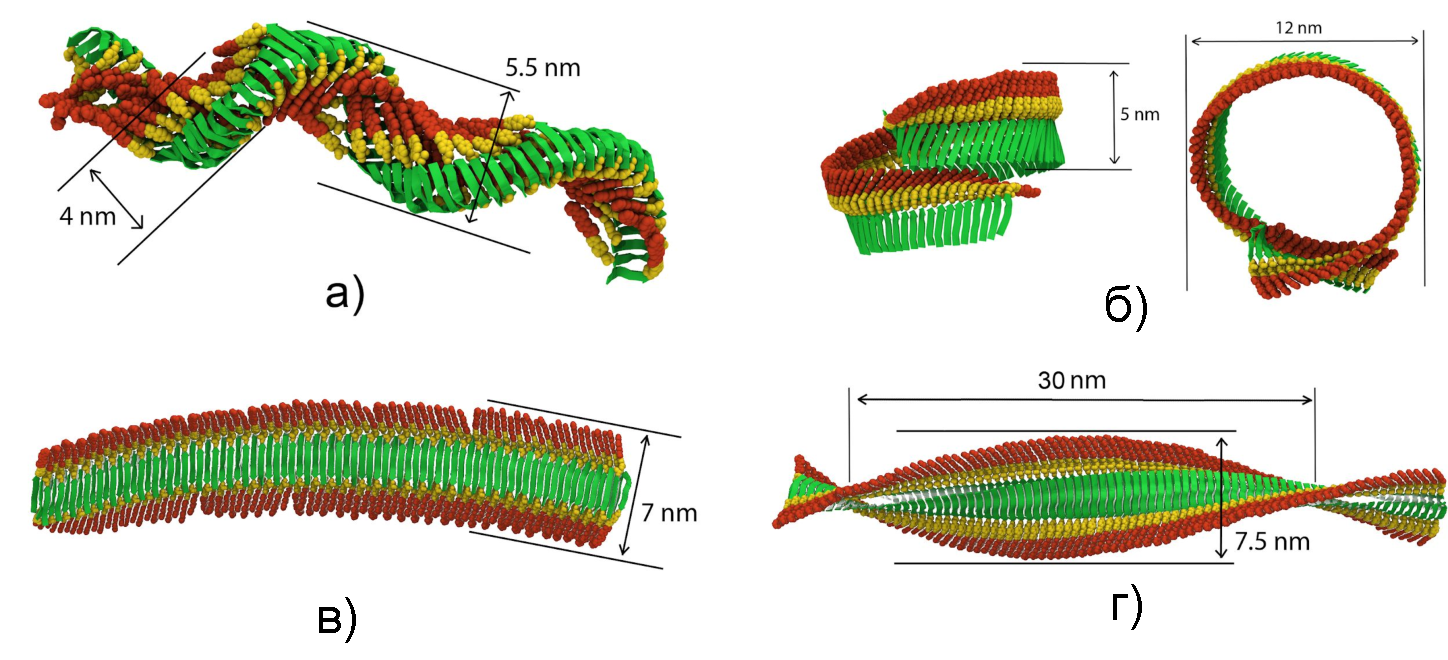
\includegraphics[width=\textwidth]{images/p4/punkt5/part4_p5_f46.pdf}
    \caption[Окончательные снимки и эволюция крупномасштабных фибрилл и их размеры]{Окончательные снимки и эволюция крупномасштабных фибрилл и их размеры: a) фибрилла типа SL-AP, б) фибрилла типа SL-PAR, в) фибрилла типа DL-AP, г) фибрилла типа DL-PAR. Алкильные хвосты не изображены, тиофеновая часть изображена красными сферами, пара-азидофенилаланинский линкер изображен желтым цветом, пептидные части изображены зелеными стрелками.}
    \label{fig:p4_p5_f46}
\end{figure}

    Постоянная длина полимерной цепи является их ключевой механической характеристикой, которая определяется как длина, на которой корреляции в направлении теряются.

\begin{equation}
    <\cos \theta(l) > = exp (-l / P)   
    \label{eq:p4:persist_len}
\end{equation}

    В формуле (\ref{eq:p4:persist_len}) P - постоянная длина, l - контурная длина полимера, $\theta$- касательный угол между точками в полимере, разделенными контурной длиной l.

    Концепция персистентной длины может также применяться для описания конформационного поведения и жесткости фибрилл. Однако это не всегда может быть сделано простым способом в нашем моделировании, поскольку некоторые из фибрилл (например, однослойные фибриллы) имеют довольно сложное конформационное поведение и потребуют очень обширной конформационной выборки. Для фибриллы DL-AP, которая демонстрирует постоянное поведение при изгибе, также необходимо расширить понятие персистентной длины.

    В этой работе мы ограничились расчетом персистентной длины фибриллы DL-PAR, поскольку это можно было сделать прямым способом, пока фибрилла, скорее всего, была прямой, и для ее описания можно применить персистентную модель гибкости полимера. Средний косинус угла между касательными как функция контурной длины показан на рисунке \ref{fig:p4_p5_f47}. Из графика видно, что средний косинус монотонно уменьшается с более резким уменьшением, когда расстояние сопоставимо с длиной моделируемой фибриллы. Последнее отклонение от экспоненциального спада объясняется концевыми эффектами. Подгонка зависимости показателем степени дает персистентную в длину 1,7 мкм. Это подтверждают экспериментальные данные, в которых персистентная длина была определена порядка микрометров. Для более подробного обсуждения см. раздел ``Обсуждение'' ниже.

\begin{figure} [H]
    \centering
    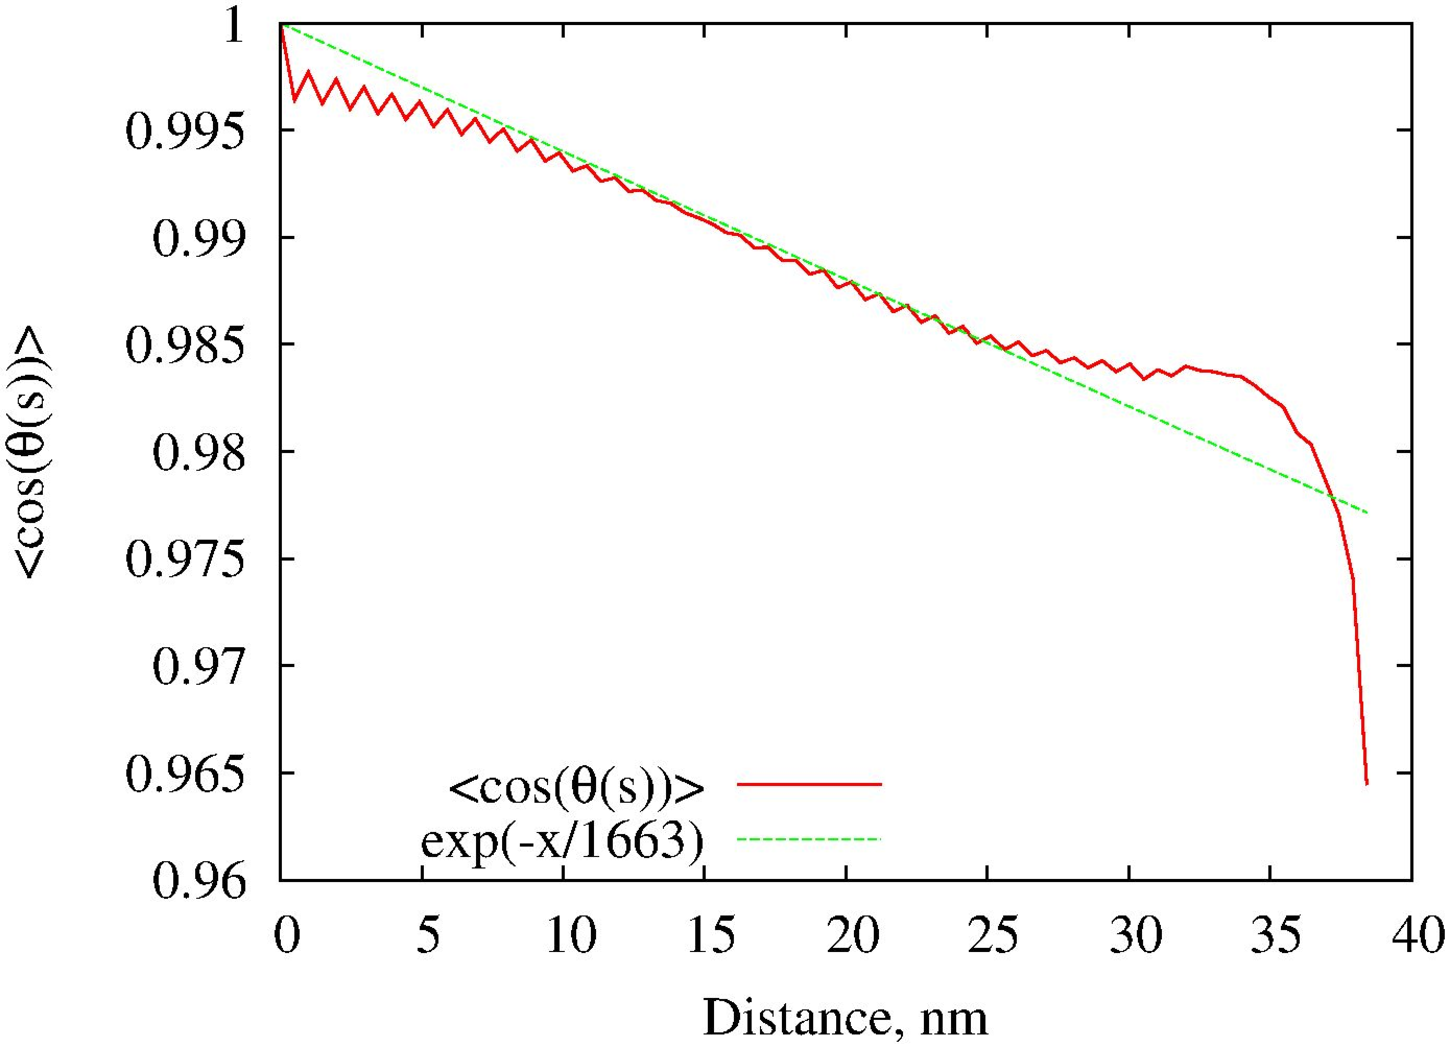
\includegraphics[width=\textwidth]{images/p4/punkt5/part4_p5_f47.pdf}
    \caption[Зависимость среднего косинуса между касательными от длины контура фибриллы для типа фибриллы DL-PAR]{Зависимость среднего косинуса между касательными от длины контура фибриллы для типа фибриллы DL-PAR, усредненного за последние 4 нс моделирования (красная линия) и аппроксимированного показателем степени (зеленая линия). Конформация фибриллы была аппроксимирована кривой, проходящей через центры масс пептидных фрагментов.}
    \label{fig:p4_p5_f47}
\end{figure}



\subsubsection{Методы}

    Моделирование длинных фибриллярных агрегатов представляет собой серьезную проблему для моделирования молекулярной динамики. Основные проблемы связаны с (i) необходимостью достаточно точного учета дальнодействующих взаимодействий и (ii) необходимостью постепенной и осторожной конформационной релаксации исходной структуры в разумные сроки. Протокол конформационной релаксации и параметры моделирования, разработанные для текущего моделирования фибрилл, описаны ниже. Для моделирования использовался пакет программ LAMMPS \cite{plimpton_fast_1995}.
    
    \textbf{Шаг 0:} Минимизация энергии молекулярной системы. Радиус обрезания для невалентных ван-дер-ваальсовых и кулоновских взаимодействий был установлен на 400\AA{} (фактически без ограничений). Минимизация энергии с использованием версии Полака-Рибиера алгоритма сопряженного градиента проводилась до тех пор, пока максимальная сила в системе не стала меньше 100 ккал/моль/А.

    \textbf{Шаг 1:} Релаксация с использованием моделирования методом МД при $T=1K$ с термостатированием на основе метода диссипативной динамики частиц (ДДЧ) в течение 0,5 нс. Радиус обрезания для невалентных ван-дер-ваальсовых взаимодействий был установлен на 20\AA, а для кулоновского взаимодействия - на 50\AA. Радиус обрезания ДДЧ-взаимодействий составлял 20\AA. Параметр трения в термостате ДДЧ был установлен на 1 $пс^{-1}$. Шаг интегрирования составлял 1 фс.

    \textbf{Шаг 2:} Релаксация с использованием МД моделирования с постепенным нагревом от $1K$ до $300K$ в течение 1 нс. Все параметры были аналогичны предыдущему шагу, за исключением изменений температуры, вызванных термостатом ДДЧ.

    \textbf{Шаг 3:} Релаксация с использованием МД моделирования при $T = 300K$ в течение 1 нс. Все параметры были аналогичны, за исключением термостата ДДЧ. Параметр трения был установлен на 0,2 $пс^{-1}$, что обеспечивало меньшее трение, чем на предыдущих этапах.
    
    \textbf{Шаг 4}: Производственный МД прогон до 10 нс. Все параметры аналогичны предыдущему шагу.
    
    
\begin{figure} [H]
    \centering
    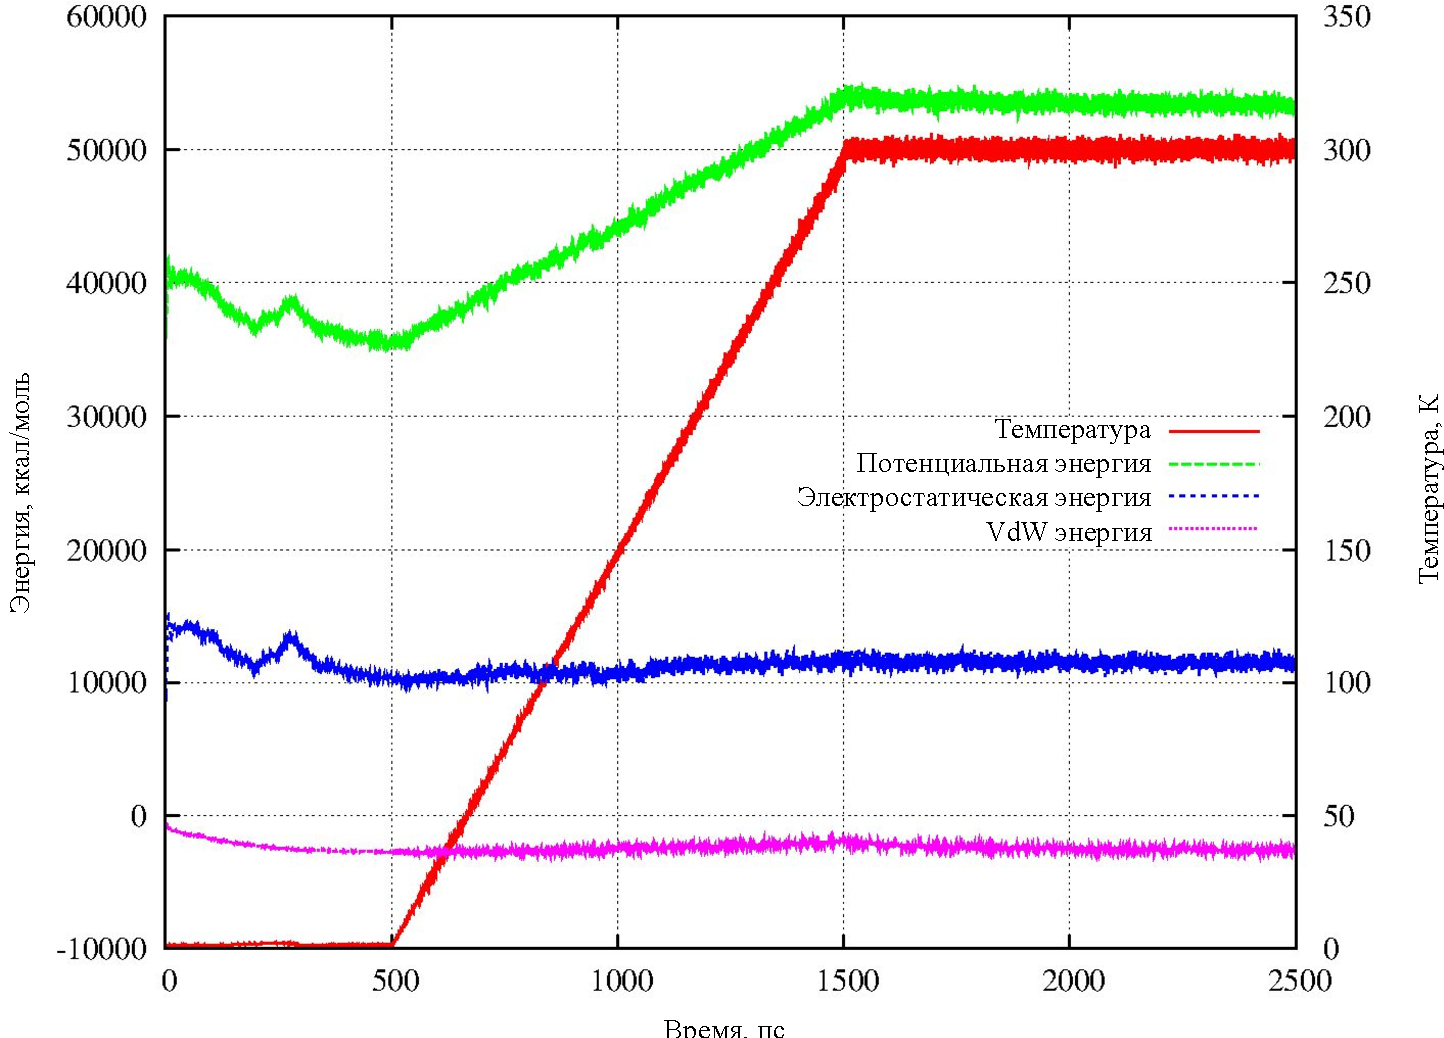
\includegraphics[width=\textwidth]{images/p4/punkt5/part4_p5_f48.pdf}
    \caption[Иллюстрация протокола моделирования МД для моделирования длинной фибриллы SL-AP]{Иллюстрация протокола моделирования MD для моделирования длинной фибриллы SL-AP. На графике показано изменение параметров энергии и температуры в течение начальных 2,5 нс моделирования.}
    \label{fig:p4_p5_f48}
\end{figure}

    Этапы релаксации 1-3 дополнительно проиллюстрированы на Рисунке \ref{fig:p4_p5_f48}, на котором показаны изменения температуры и энергии в системе во время работы. Ось времени начинается в тот же момент, что и на графиках-вставках рисунков \ref{fig:p4_p5_f43} и \ref{fig:p4_p5_f44}.


\subsection{Адсорбция агрегатов на поверхности}

    В эксперименте фибриллы обычно визуализируются с помощью атомно-силовой микроскопии (АСМ), образец наносится методом литья (drop casting) или центрифугирования из раствора на подложку. Чтобы выявить возможное влияние субстрата на морфологию фибрилл, а также понять геометрические параметры адсорбированных фибрилл, мы провели серию расчетов по имитации адсорбции.

    Длинные двухслойные фибриллы (DL-AP и DL-PAR) длиной 80 $\beta$ ($\sim$40 нм) мы поместили вблизи поверхности графита в их релаксированных конформациях и моделировали их адсорбцию.

    Используя алгоритм виртуального АСМ (см. ``Методы''), были визуализированы профили высот адсорбированных фибрилл.

\subsubsection{Результаты}

    Фибриллы были размещены в непосредственной близости от явно смоделированной поверхности графита. Исходная конформация фибрилл была принята в их наиболее благоприятном состоянии после моделирования и релаксации, описанные в предыдущем разделе. Эволюция морфологии фибрилл около подложки проиллюстрирована снимками на рис. \ref{fig:p4_p5_f49} и рис. \ref{fig:p4_p5_f50}. Адсорбция фибрилл была быстрым процессом, и после 1,5 нс моделирования фибриллы достигли своего устойчивого адсорбированного состояния.

    Как видно на рисунке \ref{fig:p4_p5_f49}, фибрилла DL-PAR, которая изначально имела скрученную конформацию, раскручивалась в процессе адсорбции и приобрела плоскую конформацию. Во время этого процесса сначала адсорбировались два конца фибриллы, а затем фибрилла разрывалась посередине, чтобы произошло полное раскручивание. Это замечательное поведение показывает, что: (i) поверхностные силы могут быть достаточно сильными, чтобы раскрутить фибриллу, (ii) фибрилла в целом является стабильным агрегатом, способным противостоять поверхностным силам, поскольку внутренняя структура фибриллы была сохранена. Фибрилла DL-AP (см. рис. \ref{fig:p4_p5_f50}) в процессе адсорбции также приобрела плоскую конформацию, но разрывов не наблюдалось, поскольку они не были необходимы с точки зрения структуры.

    Для дальнейшего анализа структуры фибриллы в адсорбированном состоянии мы представляем моментальные снимки окончательных конформаций с разных точек зрения в более подробном представлении (также с явно показанными алкильными цепями) на рисунках \ref{fig:p4_p5_f51} и \ref{fig:p4_p5_f52}.

    На снимках, визуализированных перпендикулярно оси фибрилл (рисунок \ref{fig:p4_p5_f51}б и рисунок \ref{fig:p4_p5_f51}б), видно, что геометрия поперечного сечения двух типов фибрилл различается, и конфигурация алкильных цепей играет здесь важную роль - они стерически мешают адсорбции кватротиофеновых фрагментов на графите. Для фибриллы DL-PAR сегменты кватротиофенов, а также алкильные цепи расположены согласованно с обеих сторон фибриллы - это приводит к более упорядоченной структуре и более плотной упаковке и адсорбции синтетических фрагментов на графите. Для фибриллы DL-AP из-за ее геометрии алкильные цепи образуют более неупорядоченную структуру и даже образуют промежуточный молекулярный слой между графитом и тиофенами. Различия в упаковке алкильных цепей приводят к тому, что поперечное сечение фибриллы DL-PAR толще в середине (пептидная часть), чем на краях (тиофен-алкильная часть), в то время как поперечное сечение фибриллы DL-AP имеет более прямоугольную форму.

    Чтобы улучшить понимание геометрии фибрилл, мы рассчитали виртуальные изображения АСМ, которые соответствуют адсорбированным структурам (см. Рисунок \ref{fig:p4_p5_f51}в и Рисунок \ref{fig:p4_p5_f52}в). Эти смоделированные изображения АСМ соответствуют радиусу острия кантилевера в 1 нм. Соответствующие профили высоты поперечного сечения представлены на рисунке \ref{fig:p4_p5_f53}. Четко видно, что эти профили имеют немного другую форму: профиль для фибриллы DL-PAR (рисунок \ref{fig:p4_p5_f53}a) имеет более горбовидную форму, в то время как профиль для фибриллы DL-AP (Рисунок \ref{fig:p4_p5_f53}б) имеет более прямоугольную форму.

    Виртуальные изображения АСМ также позволяют решать проблему оценки ширины и высоты фибрилл как \textit{in silico}, так и экспериментально. Из рисунков \ref{fig:p4_p5_f51}б и \ref{fig:p4_p5_f52}б видно, что ширина фибриллы составляет около 7-8 нм, хотя алкильные цепи могут простираться немного дальше. Виртуальные изображения АСМ дают более подробную информацию об этой проблеме и возможность для более прямого сравнения с экспериментальными данными, так как одно только значение ширины не слишком информативно и подвержено неточностям, связанным с конечным радиусом острия кантилевера в АСМ, а также существуют проблемы с определением ширины объектов с гладкими границами. Используя наши виртуальные АСМ изображения, предполагаемые значения ширины для фибриллы DL-PAR составляют около 8-10 нм, а для фибриллы DL-AP - около 8 нм.


\begin{figure} [H]
    \centering
    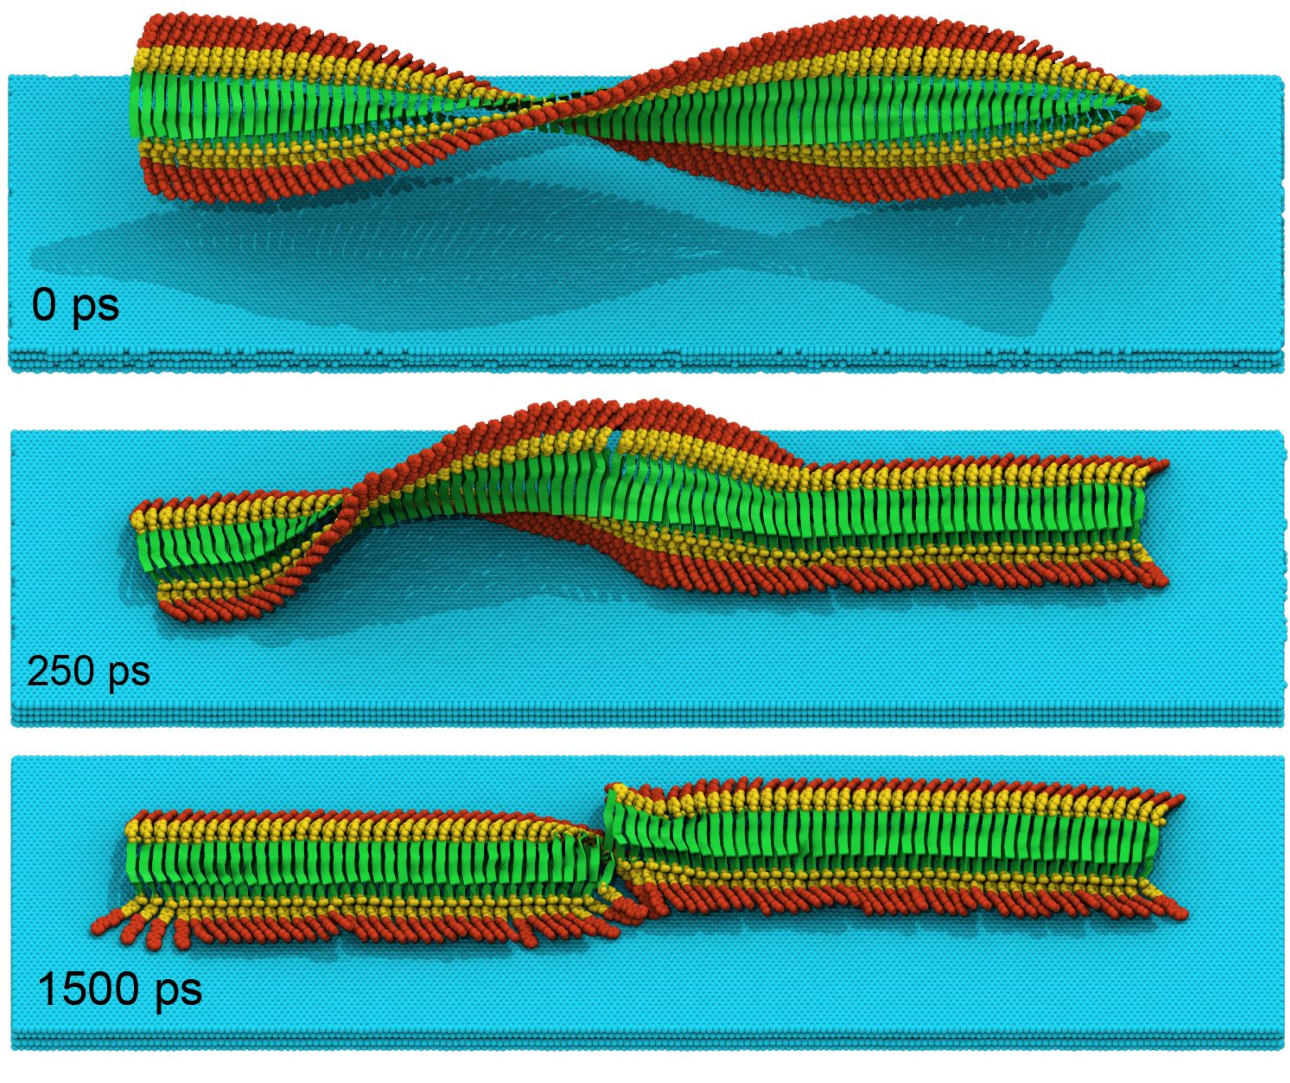
\includegraphics[width=\textwidth]{images/p4/punkt5/part4_p5_f49.pdf}
    \caption[Снимки моделирования адсорбции фибриллы DL-PAR на поверхности графита, представляющие эволюцию процесса адсорбции]{Снимки моделирования адсорбции фибриллы DL-PAR на поверхности графита, представляющие эволюцию процесса адсорбции. Поверхность графита (состоящая из 4-х слоев) окрашена в голубой цвет. Изображение фибриллы соответствует тому, что использовалось ранее. В нижнем левом углу каждого снимка указано соответствующее время моделирования.}
    \label{fig:p4_p5_f49}
\end{figure}


\begin{figure} [H]
    \centering
    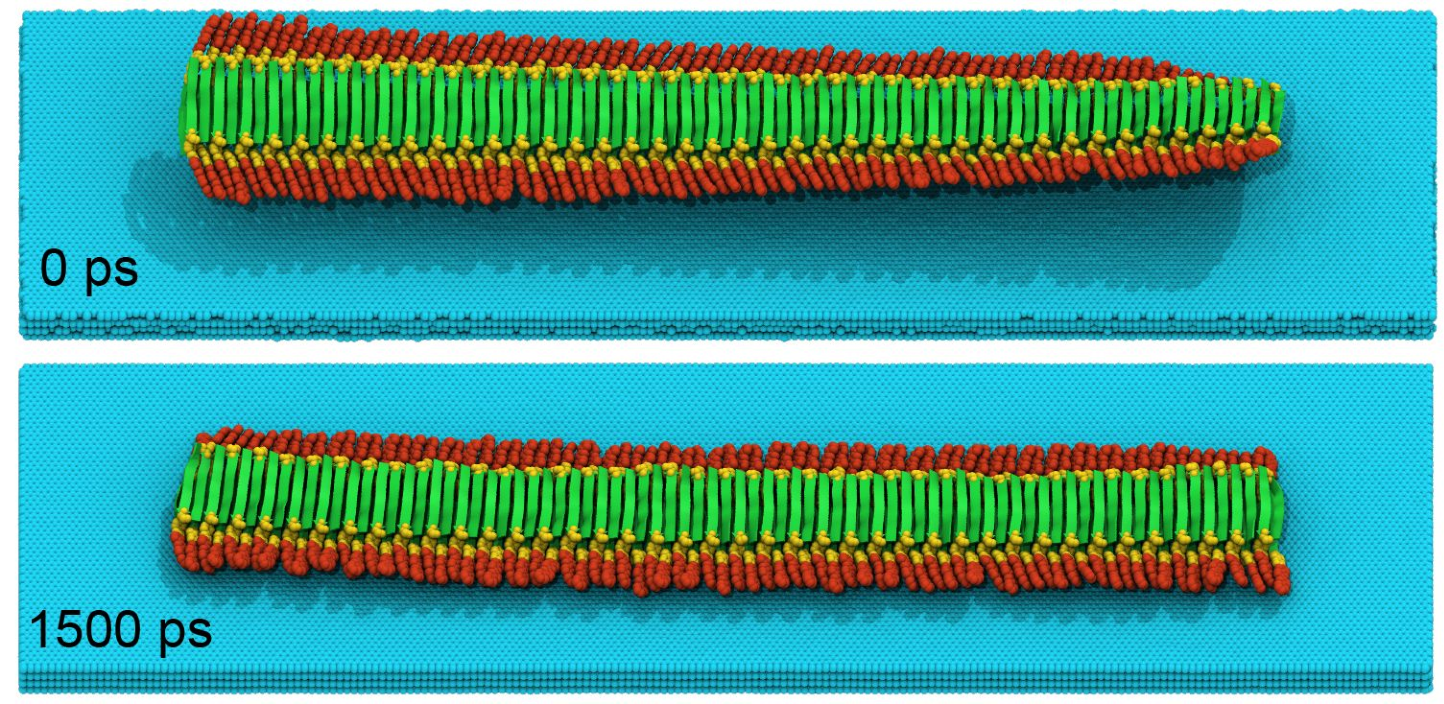
\includegraphics[width=\textwidth]{images/p4/punkt5/part4_p5_f50.pdf}
    \caption[Снимки моделирования адсорбции фибриллы DL-AP на поверхности графита, представляющие эволюцию процесса адсорбции]{Снимки моделирования адсорбции фибриллы DL-AP на поверхности графита, представляющие эволюцию процесса адсорбции. Поверхность графита (состоящая из 4-х слоев) окрашена в голубой цвет. Изображение фибриллы соответствует тому, что использовалось ранее. В нижнем левом углу каждого снимка указано соответствующее время моделирования.}
    \label{fig:p4_p5_f50}
\end{figure}


\begin{figure} [H]
    \centering
    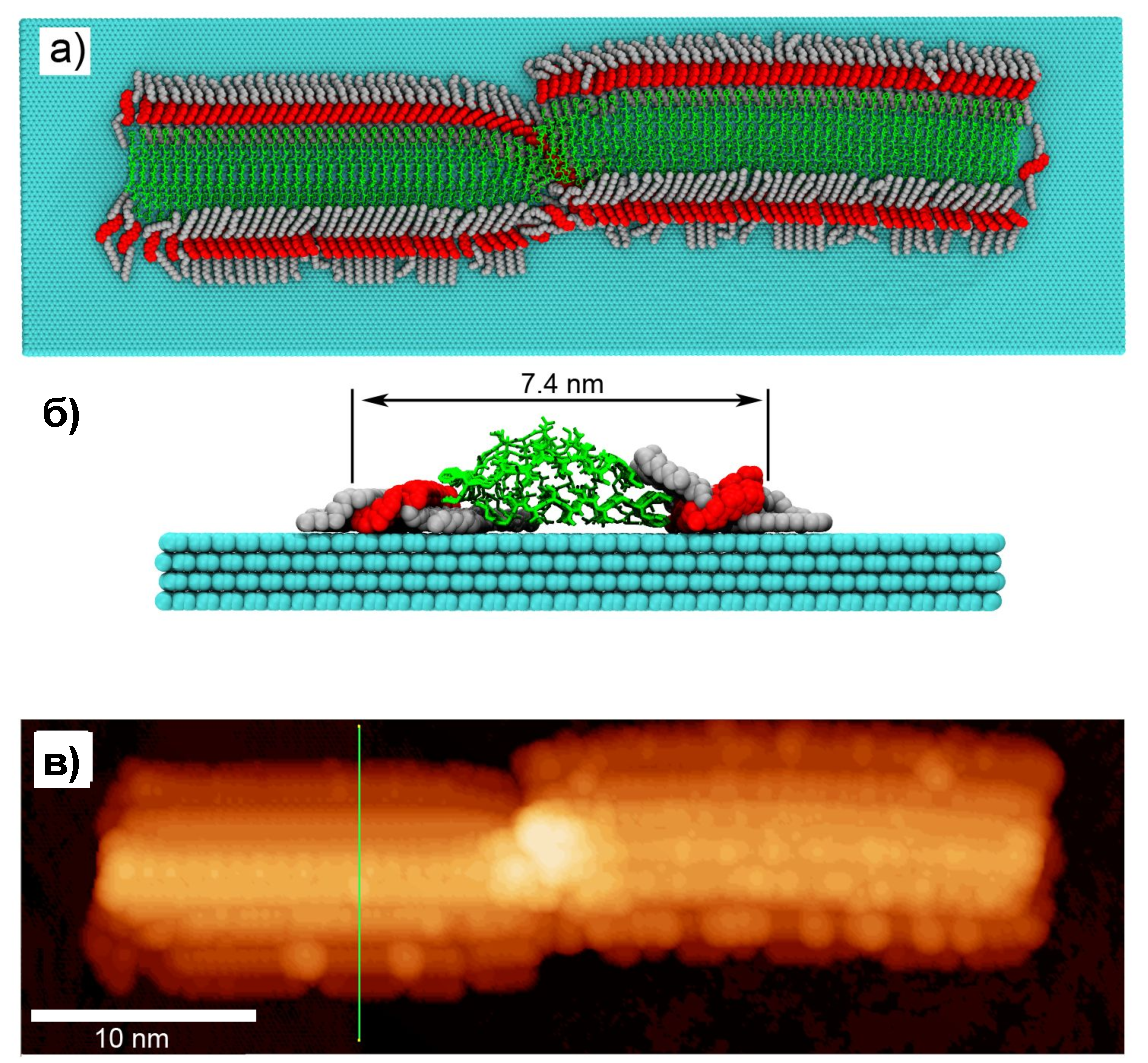
\includegraphics[width=\textwidth]{images/p4/punkt5/part4_p5_f51.pdf}
    \caption[Снимки конечного адсорбированного состояния фибриллы DL-PAR на графите]{(а), (б) - снимки конечного адсорбированного состояния фибриллы DL-PAR на графите. Графит изображен голубым, кватротиофены - красным, алкильные цепи - серым, пептидные части - зелеными трубками. (в) представлена соответствующая модель АСМ-изображения, зеленая линия соответствует поперечному сечению, представленному на рисунке \ref{fig:p4_p5_f53}a.}
    \label{fig:p4_p5_f51}
\end{figure}


    Высота фибрилл - еще один важный параметр, который можно более точно измерить в эксперименте и в меньшей степени зависит от радиуса острия кантилевера. Из наших виртуальных профилей АСМ максимальная высота фибрилл составляет 1,9 нм для фибриллы DL-PAR и 1,7–1,8\AA{} для фибриллы DL-AP.

    Дополнительные виртуальные АСМ-измерения однослойных фибрилл были выполнены путем простого отщепления верхнего молекулярного слоя. Максимальная высота однослойной фибриллы оценивается примерно в 1 нм.

    Однако следует отметить, что реальный профиль фибриллы может зависеть от многих факторов (радиуса кончика кантилевера, жесткости и амплитуды кантилевера и т. д.), поэтому при сравнении с экспериментальными данными следует проводить измерения также некоторых эталонных структур.


\begin{figure} [H]
    \centering
    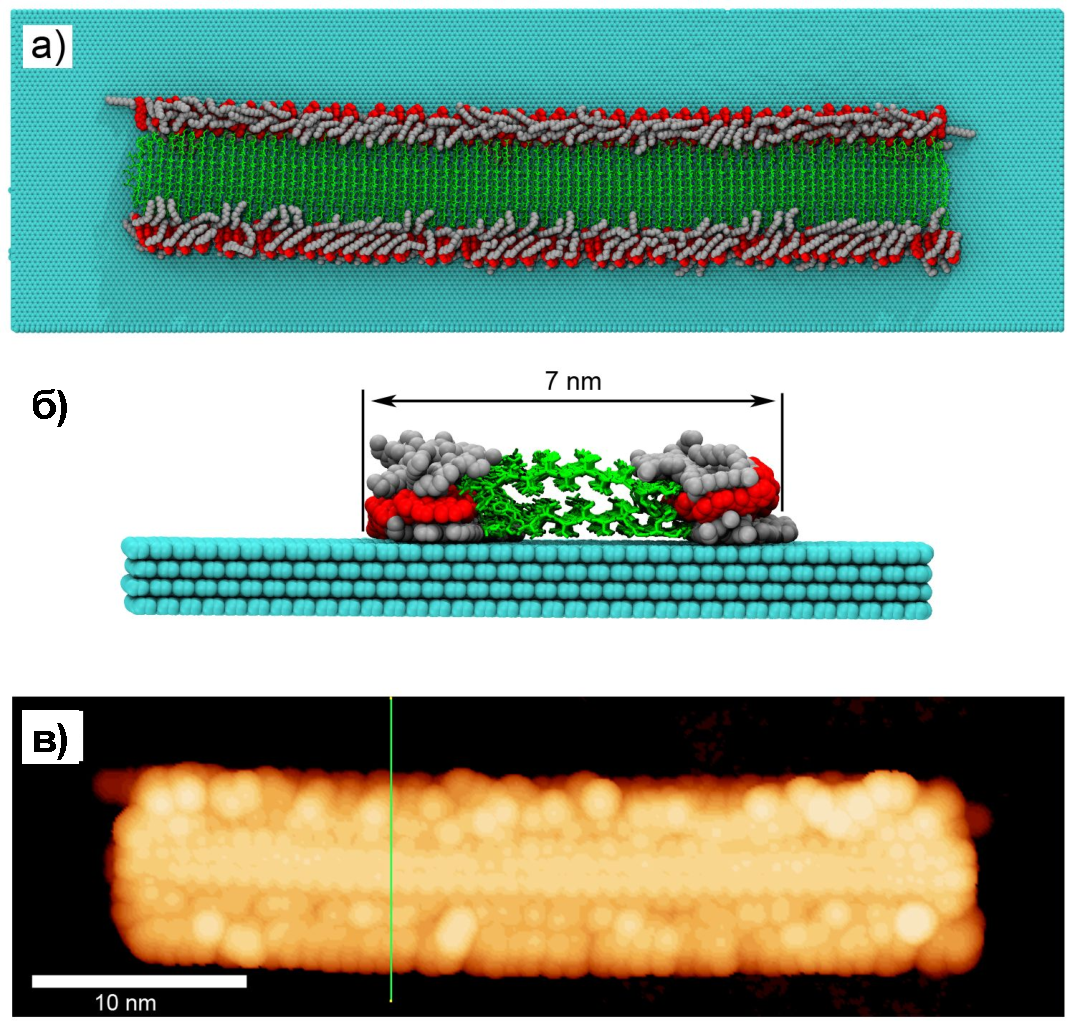
\includegraphics[width=\textwidth]{images/p4/punkt5/part4_p5_f52.pdf}
    \caption[Снимки конечного адсорбированного состояния фибриллы DL-PAR на графите]{(а), (б) - снимки конечного адсорбированного состояния фибриллы DL-PAR на графите. Графит изображен голубым, кватротиофены - красным, алкильные цепи - серым, пептидные части - зелеными трубками. (в) представлена соответствующая модель AFM-изображения, зеленая линия соответствует поперечному сечению, представленному на рисунке \ref{fig:p4_p5_f53}б.}
    \label{fig:p4_p5_f52}
\end{figure}


\begin{figure} [H]
    \centering
    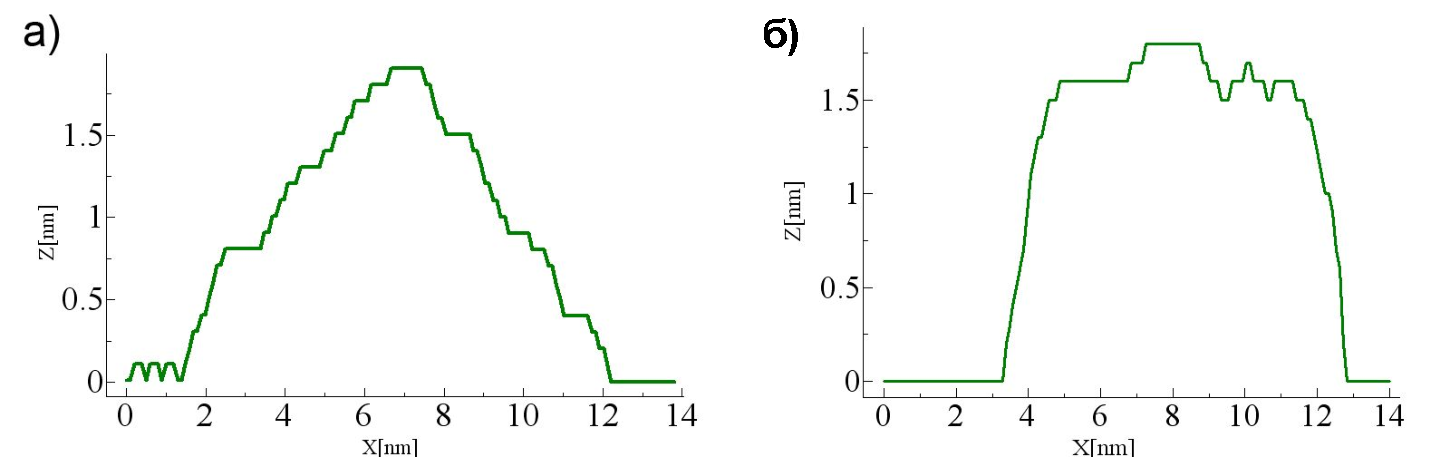
\includegraphics[width=\textwidth]{images/p4/punkt5/part4_p5_f53.pdf}
    \caption[Высотные профили поперечного сечения фибрилл, адсорбированных на графите]{Высотные профили поперечного сечения фибрилл, адсорбированных на графите, для фибрилл DL-PAR (а) и DL-AP (б). Соответствующее поперечное сечение показано на Рис. \ref{fig:p4_p5_f51}в и Рис. \ref{fig:p4_p5_f52}в зелеными линиями.}
    \label{fig:p4_p5_f53}
\end{figure}

\subsubsection{Методы}

    \emph{Построение системы и моделирование}

    Графитовая подложка была смоделирована 4 слоями графита, построенными как суперячейка из элементарной ячейки графита путем репликации ее вдоль векторов элементарной ячейки. Общие размеры подложки составляли 50 нм на 15 нм. Все моделирование проводилось с использованием метода моделирования молекулярной динамики с программным обеспечением LAMMPS и силовым полем PCFF, как описано ранее.
    
    Моделирование проводилось с периодическими граничными условиями и NVT-ансамблем. Постоянный объем, а также постоянные размеры слоев графита позволяли поддерживать подложку в вытянутой плоской форме. Невалентные взаимодействия обрабатывались следующим образом: взаимодействие Леннард-Джонса ограничивалось 10\AA, электростатическое взаимодействие обрабатывалось с помощью алгоритма PPPM \cite{hockney_computer_1989} с отсечкой в реальном пространстве 10\AA{} и значением точности $10^{-4}$. Термостат ДДЧ использовался с референсной температурой 300 К, радиусом отсечки 10\AA, а параметр трения был установлен на 0,2 $пс^{-1}$.

    \emph{Виртуальный АСМ анализ}

    Процедура виртуальных АСМ-измерений выполнялась с помощью специально разработанного программного обеспечения. В нашем алгоритме сфера зонда диаметром 1 нм приближалась к поверхности подложки в каждой точке горизонтальной сетки с шагом 0,1 нм. Затем определялось наивысшее положение зондирующей сферы, когда сфера не перекрывалась ни с одной из сфер ван-дер-Ваальса атомов в системе. Вертикальное положение сферы определялось методом деления отрезка пополам с точностью до 0,1 нм. Полученные данные были дополнительно визуализированы с помощью программного обеспечения для визуализации WSxM \cite{horcas_wsxm_2007}.

\subsection{Обсуждение}

\subsubsection{Комбинированная вычислительная/экспериментальная интегративная методология для предсказания структуры/свойств амилоидоподобных фибрилл}

    В настоящей работе мы продемонстрировали методологию мультимасштабного компьютерного моделирования для понимания структуры, морфологии и свойств конкретных фибриллярных агрегатов с ограниченными экспериментальными знаниями о межмолекулярном структурном устройстве. Методология была разработана на основе идей, сформулированных выше, и состоит из 3 этапов: (i) сначала предсказываются пробные межмолекулярные структуры, соответствующие имеющимся экспериментальным данным, (ii) фибриллы, основанные на этих структурах, затем анализируются с использованием методов мультимасштабного моделирования и (iii) их крупномасштабные свойства дополнительно сравниваются с доступными экспериментальными данными, что дает механизм обратной связи для понимания правильности первоначальных предположений. Эта методология представляет интерес сама по себе, поскольку ее можно применять не только к гибридам тиофен-пептид, но и к широкому классу амилоидоподобных волокон. В этом обсуждении мы хотели бы более подробно остановиться на особенностях методологии как комбинированного экспериментально-теоретического подхода, предназначенного для решения проблем исследования амилоидоподобных фибрилл, и описать пути его улучшения.

    Предсказание возможных начальных межмолекулярных структур - первый ключевой шаг в нашей методологии. В идеальном случае желательна пространственная структура микрокристаллов, образованных исследуемыми молекулами, решаемая с помощью рентгеновской кристаллографии или данные о пространственном расположении молекул в фибриллах, обнаруженные методом ЯМР. Однако эти наборы данных могут быть получены только в некоторых редких случаях, поэтому возможно следовать альтернативной стратегии - построение возможных укладок пептидов, согласующихся с экспериментальными данными, а затем использование методов моделирования для их оптимизации к наиболее энергетически выгодному состоянию. Данные, полученные с помощью различных экспериментальных методов, могут оказаться здесь большим подспорьем и облегчить понимание и построение схемы испытаний. Экспериментальные методы, полезные на этом этапе, сведены в Таблицу \ref{tab:p4_t3}, Часть A. Опираясь на такие экспериментальные методы, как окрашивание красителем, ИК- и КД-спектроскопия или рентгеновская дифракция и электронная дифракция, можно понять склонность образования пептидами $\beta$-листовых фибрилл и такие детали их организации, как (i) параллельная или антипараллельная организация $\beta$-листов, (ii) расстояние между стопками $\beta$-листов, если они образуют стопки, (iii) упаковка боковых цепей и т. д. Эти детали могут быть проанализированы с помощью ряда экспериментальных методов, на практике эксперименты могут быть сложными, и в некоторых случаях единственное, что мы знаем о межмолекулярном расположении, - это данные об существовании $\beta$-листов в структуре фибрилл.
    
    При построении пробных укладок на основе одиночных $\beta$-листов можно дополнительно руководствоваться основными энергетическими принципами, такими как: (i) количество водородных связей на молекулу, образованную основной цепью и боковыми цепями, (ii) возможные ионные взаимодействия между определенными заряженными остатками или концами пептида, (iii) возможные стэкинг-взаимодействия между ароматическими остатками, (iv) электростатическое отталкивание или притяжение заряженных остатков. Оптимизация предлагаемых схем испытаний должна быть проведена с использованием методов молекулярной механики и молекулярной динамики. Используя эти методы, можно дополнительно сравнить энтальпию образования различных укладок, что дает дополнительный критерий предпочтения одного устройства над другим. Если на основании экспериментальных данных предлагается укладка $\beta$-листов, то поэтапно должны быть предложены различные пробные схемы укладки на основе однослойных схем. Здесь дополнительные энергетические соображение могут направлять процесс конструирования, например, такие как (i) ионные, стэкинговые взаимодействия, водородные связи, стерические взаимодействия на границе раздела листов, (ii) влияние растворителя на укладку, включая гидрофобные взаимодействия. Здесь снова можно использовать компьютерное моделирование, чтобы оптимизировать конструкции и дать оценку предпочтения одного устройства над другим. Некоторые пробные расчеты фибрилл в растворителе и анализ взаимодействия фибрилл в растворителе (например, количество водородных связей, образованных между растворителем и фибриллой) могут дать понимание энергетической выгодности различных вариантов укладки. Вклад гидрофобных взаимодействий можно также оценить путем расчета гидрофобной поверхности, доступной для растворителя, в различных экспериментальных схемах.
    
    Однако предлагаемая в настоящее время методология по-прежнему в значительной степени зависит от подхода проб и ошибок и участия человека в процессе. В настоящее время основной проблемой является процедура оптимизации, которая носит локальный характер, поскольку она не может увести конструкцию далеко от первоначальной пробной укладки, созданной вручную. Эта проблема становится более очевидной по мере того, как структуры становятся более сложными, то есть укладкой нескольких $\beta$-листов или увеличением сложности молекул, наблюдаемых в конъюгатах пептид-полимер. Возможным  решением описанной проблемы может быть разработка специальных эффективных алгоритмов оптимизации, которые будут пытаться найти глобальный энергетический минимум молекулярного расположения, одновременно принимая во внимание экспериментальные ограничения на структурную организацию. Эти методы могут быть основаны на методах параллельного темперирования (позволяющих молекулам легко преодолевать барьеры свободной энергии) \cite{deem_parallel_2005} или параллельной оптимизации, начиная с различных случайных молекулярных конформаций, как это используется в пакете GULP \cite{gale_general_2003}. Идеальным была бы своего рода комбинация подходов, когда автоматический прогноз кристаллической упаковки можно было бы адаптировать к прогнозированию одномерных амилоидных фибрилл и в то же время учитывать ограничения, исходящие из экспериментальных данных
    
    
%TABLE3------------------------------------------------------------
\begin{table}[H]
    \centering
    \begin{tabularx}{\textwidth}{|X|X|}
        \textbf{Экспериментальный подход} & \textbf{Полезные данные} \\
\hline
        \multicolumn{2}{l|}{\textbf{Часть A}-методы выявления межмолекулярной структуры} \\
\hline
        КД-спектроскопия & Обнаруживает наличие $\beta$-листов \\
\hline
        ИК-спектроскопия & Обнаруживает наличие $\beta$-листов, возможно, может различать параллельные и антипараллельные $\beta$-листы \\
\hline
        УФ-видимая спектроскопия & При окрашивании конго красным возможно обнаружение амилоидов \\
\hline
        Флуоресцентная спектроскопия & При окрашивании Тиофлавином Т или Конго красным возможно обнаружение амилоидов \\
\hline
        Рентгеновская дифракция на порошке или волокнах & Шаг-листов, укладка $\beta$-листов, упаковка боковой цепи, параллельное или антипараллельное расположение \\
\hline
        Окрашивание красителем (Конго Красный, Тиофлавин Т) & Обнаружение наличия амилоидов \\
\hline
        Электронная дифракция & Шаг $\beta$-листов, укладка $\beta$-листов \\
\hline
        Модификация химической структуры, зависимость самосборки от различных параметров (растворитель, температура) & Может выявить ключевые меж- и внутримолекулярные взаимодействия, а также влияние растворителя на самосборку - преобладание полярных или гидрофобных взаимодействий. \\
\hline
       \multicolumn{2}{l|}{\textbf{Часть B} - методы визуализации свойств волокна}\\
\hline
        Атомно-силовая микроскопия & Размеры фибрилл, параметры скручивания (возможное влияние поверхности) \\
\hline
        Просвечивающая электронная микроскопия & Размеры фибрилл, параметры скручивания (возможное влияние субстрата) \\
\hline
        Криофиксирующая электронная микроскопия & Размеры фибрилл, параметры скручивания \\
\hline
    Рассеяние нейтронов и рентгеновских лучей & Размеры фибрилл, структурные факторы \\
\hline
    \end{tabularx}
    \caption{Экспериментальные методы, используемые для изучения амилоидных фибрилл, а также ценные данные, которые могут быть получены и использованы в обсуждаемой методологии. Для дальнейшего обсуждения методов см. также \cite{sigurdsson_amyloid_2005}.}
    \label{tab:p4_t3}
\end{table}

    
    Следующим шагом в нашей многомасштабной методологии является моделирование фибрилл на основе предсказанных межмолекулярных структур в объеме растворителя. Основная цель такого моделирования состоит в том, чтобы (i) проверить стабильность фибрилл в среде растворителя, (ii) оптимизировать и изучить межмолекулярную структуру молекул в фибриллярном состоянии, (iii) выявить и изучить супрамолекулярную морфологию фибрилл в различных средах (например, на подложке).
    
    Опыт, собранный в этой работе, показывает, что наиболее важные проблемы при моделировании фибрилл проистекают из (i) их большого пространственного масштаба, который делает моделирование требовательными к вычислительных ресурсам, (ii) важности дальнодействующих взаимодействий для супрамолекулярной морфологии, правильное рассмотрение которых может значительно увеличить необходимость в вычислительных ресурсах, (iii) крупномасштабные конформационные переходы, которые могут происходить во время релаксации фибрилл, требующие особого внимания, (iv) для моделирования без явного растворителя, большинство алгоритмов термостатирования не подходят. В попытке сбалансировать эти проблемы мы предложили двухэтапный подход к моделированию, который включает (i) моделирование фибрилл среднего размера (длиной около 20 $\beta$-нитей) в явном растворителе и (ii) моделирование одиночных фибрилл (около 80 $\beta$-нитей) без явного растворителя. Моделирование в растворителе позволяет оценить стабильность и основные конформационные свойства фибрилл, а также описать взаимодействия растворитель-фибрилла и дополнительно оптимизировать структуру фибрилл в присутствии растворителя. Однако поведение коротких фибрилл в этих симуляциях нельзя с уверенностью экстраполировать на более крупные масштабы, поскольку (i) конформационное поведение может быть искажено краевыми эффектами и эффектами конечного размера, и (ii) некоторые конформационные черты могут быть даже не видны в этих условиях, например небольшие значения осевого скручивания, которое для многих амилоидных волокон может составлять всего $1-2^{\circ}$ на $\beta$-слой \cite{paravastu_molecular_2008}, или эффекты более крупного масштаба, такие как образование суперспирали и т. д. Следовательно, необходимы некоторые крупномасштабные расчеты, однако с ними имеется несколько очевидных проблем: (i) моделирование в явном растворителе непрактично, поскольку необходимы очень большие системы для моделирования, и требуется гораздо большее время моделирования, чтобы наблюдать большие конформационные перестройки, которые могут иметь место, потому что они будут затруднены временными масштабами перегруппировки растворителя , (ii) схемы расчета для невалентных взаимодействий (ван-дер-ваальсово-кулоновское) следует применять с осторожностью, поскольку в одномерных периодических системах заряды скоррелированы в пространстве на больших расстояниях, и дальнодействующие взаимодействия играют важную роль в формировании крупномасштабной морфологии (например, скручивания), (iii) протоколы релаксации (включая алгоритмы термостатирования) для изначально планарных фибрилл должны быть тщательно выбраны, поскольку резкая релаксация напряжений в фибрилле может привести к непредсказуемым результатам. Чтобы частично решить эти проблемы, мы ввели метод моделирования фибрилл с помощью термостата ДДЧ и специальный протокол релаксации, который оказался простым и ценным методом. Термостат ДДЧ позволяет эффективно имитировать кинетические эффекты растворителя и управлять конформационной релаксацией фибриллярной структуры предсказуемым и плавным образом за короткий период времени.
    
    Точность наших моделей в вакууме не лишена некоторых ограничений. Во-первых, в нашем моделировании не учитывались энергетические эффекты растворителя, они могут перенормировать электростатические взаимодействия между молекулами фибриллы из-за диэлектрической проницаемости растворителя, а также вызвать некоторые взаимодействия, опосредованные растворителем. Однако мы не думаем, что включение растворителя изменило бы качественное поведение фибрилл при моделировании радикально (хотя диэлектрическая проницаемость смеси метанола и дихлорметана составляет около 20), поскольку конформации фибрилл, наблюдаемые при моделировании в растворителе и вакууме в нашем исследования были согласованы. Параметры осевого скручивания, измеренные при моделировании в вакууме и растворителе, хотя и различались, например, для фибриллы DL-PAR измеренное закручивание в растворителе составило около 4,5 на $\beta$-нить, тогда как при моделировании в вакууме около $2,8^{\circ}$ на $\beta$-нить. Однако это различие также может быть связано с эффектами конечного размера, присутствующими в небольших фибриллах. В любом случае для моделирования в растворителях с более высокой диэлектрической проницаемостью и в воде может быть рекомендовано использование неявных моделей растворителей там, где это возможно.
    
    Во-вторых, крупномасштабная конформационная эволюция фибрилл может иметь несколько путей и зависеть от условий исходной конформации, а также от кинетических свойств неявной среды (термостат ДДЧ), особенно для конформационно гибких фибрилл, таких как однослойные. Например, SL-AP, начиная свою эволюцию из идеально прямой конформации, сворачивается в левую суперспираль, однако, если из-за некоторых начальных условий начальные колебания приведут фибриллу к правой суперспирали, она может продолжить этот кинетический путь. Учитывая это, следует проявлять осторожность при создании начальных структур, которые не имеют предпочтения ни к одному из крупномасштабных морфологических состояний. Также рекомендуется начать несколько расчетов с разными случайными начальными числами для термостата ДДЧ или генерации начальной скорости.
    
    Дополнительный метод моделирования, который мы ввели, - это моделирование фибрилл на графитовой подложке после их релаксации в вакууме. Этот метод был предназначен для имитации стандартной экспериментальной процедуры, когда фибриллы, уже образовавшиеся в растворе, наносятся методом центрифугирования на подложку и там анализируется их морфология. Соответствие фибриллярной структуры в растворе и на подложке в настоящее время является предметом дискуссий (см., например, \cite{borner_organization_2008}). Однако считается, что структура фибрилл из конъюгатов полимер-пептид, полученных с помощью АСМ-изображений, должна соответствовать структуре фибрилл в растворе, и кручение фибрилл часто можно увидеть на АСМ-изображениях \cite{diegelmann_one-dimensional_2008,schillinger_oligothiophene_2009}. Здесь мы показали, что это может быть не всегда. \textit{Скрученные в растворе фибриллы могут разорваться и раскрутиться под действием поверхностных сил.}
    
    Соответствующие свойства фибрилл, полученные при моделировании растворителя, вакуума или подложки, такие как ширина, высота, шаг спирали и угол спирали, можно сравнить со свойствами, полученными экспериментальными методами, приведенными в таблице \ref{tab:p4_t3}, часть Б. Это сравнение обеспечивает механизм обратной связи, для оценки правильности моделирования и прогнозируемой структуры.
    
    В заключение мы хотели бы подчеркнуть, что одно компьютерное моделирование все еще не может предоставить окончательный инструмент, который может предсказать структуру, свойства и морфологию амилоидоподобных фибрилл, исходя только из химической структуры молекул, однако сочетание экспериментальных методов с методами моделирования в синергетической методологии исследования могут стать таким инструментом и даже в большей степени инструментом для рационального дизайна фибрилл с заданными свойствами для нужд био- и нанотехнологий. Идея такой методологии проиллюстрирована на схеме рисунке \ref{fig:p4_p5_f54}.
    
\begin{figure} [H]
    \centering
    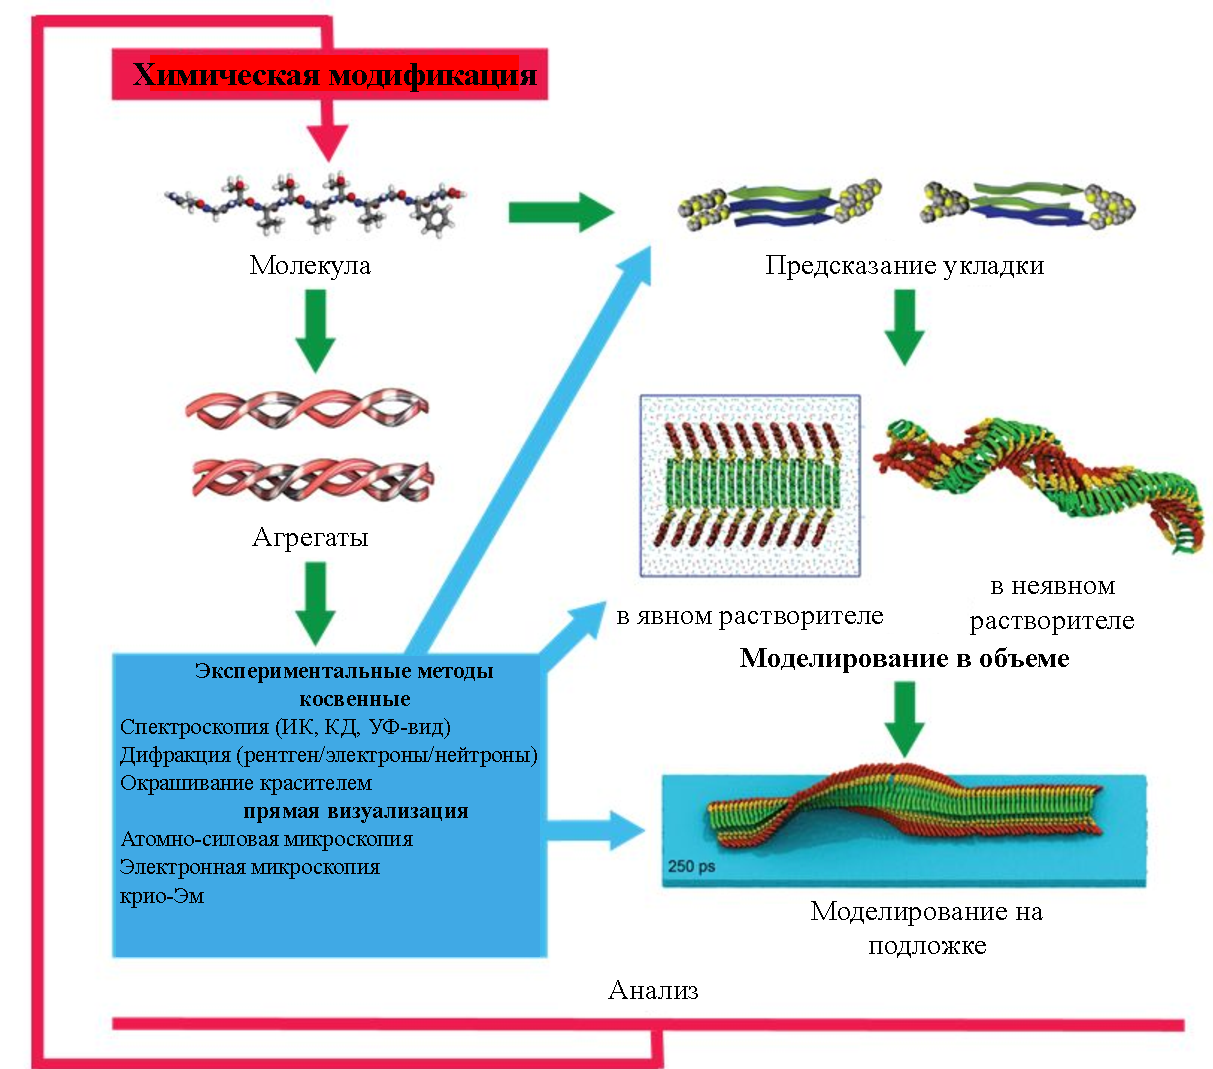
\includegraphics[width=\textwidth]{images/p4/punkt5/part4_p5_f54.pdf}
    \caption[Схематическое изображение комбинированной экспериментальной/вычислительной интегративной методологии для изучения амилоидоподобных фибрилл]{Схематическое изображение комбинированной экспериментальной/вычислительной интегративной методологии для изучения амилоидоподобных фибрилл.}
    \label{fig:p4_p5_f54}
\end{figure}
    
    
\subsubsection{Соотношения структура-морфология-свойства в фибриллах, образованных тиофен-пептидными олигомерами}
    
    Многоуровневое моделирование тиофен-пептидных агрегатов выдвинуло на первый план основные принципы организации этих фибриллярных агрегатов, включая детальное взаимодействие между межмолекулярной организацией кватротиофеновых и пептидных блоков и его влияние на структуру, морфологию и свойства фибрилл. Ниже мы обсуждаем наблюдаемые результаты.
    
    \emph{Паттерны самосборки гибридных фибрилл и иерархия взаимодействий}
    
    Хотя образование $\beta$-листов пептидными частями наших молекул изначально предполагалось в нашей методологии, дальнейшее моделирование доказало, что фибриллы стабильны как в вакууме, так и в растворе. Эволюция фибрилл и сравнительный анализ организации пептидной и тиофеновой частей фибрилл ясно показали, что в структуре и морфологии фибрилл доминируют взаимодействия пептид-пептид, а не взаимодействия тиофен-тиофен. Поскольку самосборка $\beta$-нитей в $\beta$-листы по-прежнему является основной движущей силой самоорганизации наших гибридных молекул, мы утверждаем, что иерархический механизм самосборки последних может быть описан аналогично предложенному Аггели и др. для чистых пептидных фибрилл \cite{aggeli_hierarchical_2001}. В подходе статьи \cite{aggeli_hierarchical_2001} вводится иерархия взаимодействий, а также последовательная иерархия агрегатных структур с увеличением концентрации мономера (см. Рисунок \ref{fig:p4_p1_f5}). Предполагается, что следующее неравенство
    
\begin{equation}
    \varepsilon_{tape} \gg kT \gg \varepsilon_{ribbon} \gg \varepsilon_{fibril} \gg \varepsilon_{fiber}
\end{equation}
    
    выполняется для соответствующих энергий, в расчете на один пептид внутри соответствующих структур по сравнению с пептидом внутри структуры предыдущего уровня.
    
    В обозначениях, введенных Aggeli et al. в нашем моделировании исследовались только агрегаты типа лент и и двойных лент. Из результатов моделирования можно предположить, что присоединение синтетических частей к пептидным частям вряд ли влияет на основные принципы организации на этих уровнях. Однако эффекты вполне вероятно будут проявлятся на более высоких уровнях организации, когда филаменты должны взаимодействовать друг с другом.
    
    В то же время на этих более низких уровнях самоорганизации введение синтетической части может изменить баланс между различными способами самосборки, например параллельная и антипараллельная организация нитей, укладка лент с разных сторон. Как было показано в нашем моделировании с растворителем, взаимодействие растворителя-фибриллы также может играть важную роль в выборе предпочтительного режима самосборки.

    Следует иметь в виду, что уровень иерархии, достигаемый самосборкой мономеров, зависит от концентрации мономеров, поэтому при более низких концентрациях в эксперименте мы можем видеть только отдельные ленты, в то время как на высоких концентрациях -- волокнах с высокой сложностью.
    
    Электростатические и дипольные взаимодействия, по-видимому, также важны для определения паттерна самосборки фибрилл. Даже если концы пептида не заряжены, каждая $\beta$-цепь имеет небольшой дипольный момент, направленный от С-конца (частично отрицательный) к N-концу (частично положительный). Таким образом, энергетически выгодно, когда дипольные моменты соседних $\beta$-нитей антипараллельны, это может быть достигнуто либо путем использования антипараллельной организации $\beta$-листов, либо путем наложения вместе параллельных $\beta$-листов таким образом, чтобы дипольные моменты соседних листов компенсированли друг друга.
    
    \emph{$\pi - \pi$-стэкинг по сравнению с водородными связями}
    
    Что касается приложений, наиболее интересным аспектом представленной здесь работы является расположение конъюгированных тиофеновых фрагментов и взаимодействие между $\pi - \pi$-укладкой и образованием $\beta$-листа. Расстояние между пептидными цепями, обусловленное структурой $\beta$-листа, соответствует 4,7-5\AA, в то время как расстояние между $\pi$-сопряженными плоскостями олиготиофенов для взаимодействий $\pi - \pi$-стэкинга оценивается методами квантовой химии и в идеале составляет примерно 3,3-3,5\AA{} \cite{rodriguez-ropero_ab_2008,tsuzuki_model_2002}. Следовательно, эти взаимодействия могут демонстрировать конкурирующее поведение с точки зрения периодичности, подразумеваемой во время молекулярной агрегации, и это несоответствие периодичности должно быть как-то разрешено. Анализ гистограмм распределения расстояний между центрами масс пептидов, а также между кватротиофенами (рис. \ref{fig:p4_p5_f40}) ясно выявил преобладание периодичности, подразумеваемой для агрегатов за счет расположения пептидов $\beta$-листах для всех типов моделируемых фибрилл.
    
    Сила и происхождение взаимодействий $\pi - \pi$-стэкинга в плоских ненасыщенных органических молекулах до сих пор остаются предметом споров. В  \cite{grimme_special_2008} было показано, что для относительно небольших ароматических систем (менее 10-15 атомов углерода) стэкинг-взаимодействия могут быть описаны чисто дисперсионными взаимодействиями (силы ван-дер-Ваальса) и только для более крупных систем появляется определенный дополнительный энергетический вклад на малых расстояниях стэкинга, вступает в игру эффект электронной корреляции. В наших симуляциях мы были в пределах чисто ван-дер-ваальсова описания стэкинга, поскольку не могли быть включены эффекты электронной корреляции. Однако, поскольку кватротиофены являются относительно небольшими сопряженными молекулами, мы надеемся, что это хорошее приближение к реальности.
    
    Чтобы понять качественное поведение кватротиофена только в стопке, мы провели моделирование минимизации энергии собранной стопки кватротиофенов с использованием того же силового поля PCFF, что и в моделировании фибрилл. Полученное межплоскостное расстояние тиофенов составило 3,55\AA, что не противоречит расчетам квантовой химии. Кватертиофены, однако, также были смещены латерально по отношению к соседней молекуле на 1,4\AA{} в направлении длинной оси (направление x) и на 1,8\AA{} в перпендикулярном направлении (направление y).
    
    Эти значения можно сравнить со значениями, определенными для расположения тиофена в фибрилле. Видно, что среднее расстояние между плоскостями тиофена (среднее смещение z) все еще составляет около 3,5\AA, что соответствует типичному расстоянию стэкинга $\pi - \pi$. Как этого произошло? В случае параллельного расположения-цепей (см. рис. \ref{fig:p4_p5_f41}б,г) тиофеновые фрагменты наклоняются синхронно, таким образом одновременно сохраняя высокую степень упорядоченности и выполняя ограничения периодичности, накладываемые $\beta$-листами. Однако это происходит за счет дополнительного бокового смещения по сравнению со значениями идеальной стопки. В случае антипараллельного расположения предлагаемая двухслойная фибрилла (рис. \ref{fig:p4_p5_f41}в) в принципе имеет такую же линейную плотность кватротиофенов вдоль фибриллы, как и в случае фибрилл с параллельным расположением, поскольку тиофеновые фрагменты обеих лент соприкасаются для образования ``стерической молнии'' вдоль каждой стороны двойной ленты (олиготиофеновые фрагменты с обеих сторон находятся в чередующемся контакте). Однако при антипараллельном расположении части тиофена имеют тенденцию наклоняться друг к другу, образуя динамические кластеры с промежутками между отдельными кластерами; такое расположение уменьшает различия между оптимальными интертиофеновыми и межпептидными расстояниями. С другой стороны, из-за этой тенденции к формированию динамических кластеров степень дальнего порядка в расположении олиготиофена значительно ниже для фибрилл с антипараллельным расположением, чем для фибрилл с параллельными $\beta$-нитями.
    
    Другой интересный пример влияния пептидной организации на упорядочение тиофенов - это влияние скручивания фибрилл на расстояние между кватротиофенами. Из рисунка \ref{fig:p4_p5_f40}г видно, что среднее расстояние между тиофенами в скрученной фибрилле даже больше, чем периодичность $\beta$-листов по чисто геометрическим причинам. Поскольку края скрученной ленты нужно растягивать больше, чем центральную часть.
    
    \emph{Кручение и изгиб фибрилл}
    
    Осевое скручивание - это внутреннее свойство $\beta$-листовых структур, возникающее в основном из-за хиральности аминокислот. Предполагается, что скручивание связано с чередующимися колебаниями двугранных углов, чтобы предотвратить расхождение отдельных $\beta$-нитей в более крупном листе \cite{he_mathematics_2011}, однако в литературе также предлагались другие вклады в угол закручивания, включая энтропию, связанную со степенями свободы остова \cite{chothia_conformation_1973}, внеплоскостная деформация пептидных групп \cite{salemme_structural_1983}, внутрицепочечные \cite{chou_role_1983}, третичные взаимодействия \cite{yang_free_1995,wang_molecular_1996}, тенденция к минимизации площади поверхности системы \cite{koh_minimal_2005}. Однако точное понимание зависимости твиста от молекулярной организации все еще остается не вполне понятным. В пионерских исследованиях геометрии $\beta$-листов было предсказано большее скручивание для антипараллельных листов \cite{chou_origin_1982}, однако современные данные предполагают, что проблема намного сложнее, например, граница раздела между двумя листами может значительно влиять на степень скручивания. и даже обратить тенденцию вспять \cite{berryman_prediction_2008}. Также утверждается, что экспериментально наблюдаемое скручивание в фибриллах может возникать не только из-за изменения симметрии упаковки, но также потенциально из-за кинетического захвата в состояниях, которые имеют твист, отличный от глобального минимума \cite{berryman_prediction_2008}. Периодическое кручение в классических амилоидных волокнах обычно наблюдается на масштабах в сотни нанометров \cite{paparcone_microscale_2009}.
    
       В целом левая закрутка амилоидных фибрилл, построенных на основе левозакрученных $beta$-нитей, соответствует представлениям о часто наблюдающемся хиральном дуализме и чередовании хиральности при иерархическом структурообразовании биологических систем \cite{tverdislov_chiral_2016}.
    
    Как показало молекулярное моделирование, фибриллы, образованные нашими гибридными молекулами тиофен-пептид, также могут проявлять скрученное поведение. В случае фибриллы DL-PAR наблюдалось четкий период кручение в 60 нм (плоскость ленты поворачивается примерно на $360^{\circ}$), в то время как для фибриллы DL-AP можно было бы предположить период кручения около 170 нм, хотя это сопровождается изгибом ленты. Эти значения находятся в диапазоне значений, обычно наблюдаемых в амилоидных фибриллах. Происхождение этого скручивания может быть дополнительно выяснено путем сравнения этих симуляций с отдельным исследованием симуляции, в котором рассматривалась только пептидная часть фибриллы. При сравнении окончательных структур фибрилл, представленных на рис. \ref{fig:p4_p5_f44} и рис. \ref{fig:p4_p5_f45}, становится очевидным, что: (i) степень скручивания фибриллы DL-PAR не изменяется алкил-тиофеновыми фрагментами, (ii) пептидная фибрилла в случае DL-AP не скручена и не изогнута, в то время как добавление алкил-тиофеновых фрагментов вызывает изгиб фибриллы, который сопровождается осевым скручиванием, но гораздо меньшим, чем в случае фибриллы DL-PAR. Делать некоторые общие выводы из анализа этих двух случаев было бы преждевременным, но мы можем указать на некоторые возможные тенденции в изменении морфологии фибрилл из-за добавления синтетической части. Мы утверждаем, что если бы фибрилла имела четко выраженное скручивание, уже происходящее из взаимодействия ее пептидных фрагментов (с соответствующей упругой энергией, связанной со скручиванием), добавление алкил-тиофеновых фрагментов к химической структуре вряд ли изменило бы это поведение скручивания серьезным образом. Мы должны снова учитывать, что скручивание фибриллы не способствует плотной упаковке тиофеновых фрагментов, связанных с пептидами, однако ван-дер-ваальсово взаимодействие, ответственное за упаковку тиофена, не велико и не перевешивает потерю изгибной энергии пептидной части фибриллы, которая может быть вызвана раскручиванием фибриллы.
    
    С другой стороны, если пептидная часть фибриллы не проявляет значительного предпочтения к скручиванию, факторы, связанные с упаковкой тиофенов, становятся более важными для определения общей формы фибриллы. Поскольку даже небольшие взаимодействия могут возмущать структуру и вызывать ее скручивание-искривление, но в больших пространственных масштабах.
    
    Еще один момент, который следует упомянуть, - это различие между однослойным и двухслойным расположением - кажется, что осевое скручивание происходит из тонкого баланса различных взаимодействий, поэтому данные об осевом скручивании однослойных фибрилл не могут быть экстраполированы на двухслойные. Это хорошо видно при сравнении их поведения в наших расчетах.
    
    \emph{Персистентная длина фибрилл}
    
    В то время как для однослойных фибрилл трудно определить персистентную длину из компьютерного моделирования из-за высокой конформационной лабильности последних и, следовательно, сложного механизма гибкости, для двухслойных фибрилл могут быть применены идеи простого механизма персистентной гибкости. Значение 1,7 мкм было получено при моделировании фибриллы DL-PAR. К сожалению, точное измерение постоянной длины было невозможно в эксперименте, однако по изображениям фибрилл, полученным методом АСМ, можно предложить оценку в несколько микрометров, которая хорошо согласуется. В специальных исследованиях родственных им биологических амилоидных фибрилл были получены точные численные значения персистентной длины, которые составляют от 3 до 12 мкм в зависимости от типа фибриллы, что еще раз подтверждает наш вывод \cite{knowles_spatial_2006}.
    
    \emph{Влияние адсорбции субстрата на фибриллы}
    
    Одним из наиболее распространенных методов визуализации фибриллярных структур является атомно-силовая микроскопия, которая требует осаждения фибрилл на подложку, обычно мусковитовую слюду или высокоориентированный пиролитический графит. Следовательно, влияние взаимодействий субстрат-фибрилла на морфологию агрегатов важно для интерпретации экспериментальных результатов. Из результатов нашего моделирования мы можем предположить, что для двухслойных фибрилл силы поверхностной адсорбции достаточно велики, чтобы изменить скрученную морфологию фибрилл на плоскую и даже разорвать фибриллы в процессе адсорбции. Это ставит вопрос о том, можно ли экстраполировать данные о морфологии фибрилл, полученные методами АСМ или ПЭМ в сухом состоянии, на состояние фибрилл в растворе.
    
    В Börner et al. \cite{borner_organization_2008} сравнили размеры и морфологию фибрилл из конъюгатов поли (этиленоксид) -пептид, полученных с помощью АСМ и ПЭМ в сухом состоянии, с данными, полученными с помощью просвечивающей электронной микроскопии с криофиксацией и малоуглового рассеяния нейтронов. Авторы предполагают, что АСМ и методы ПЭМ достаточно надежны, чтобы судить о морфологии фибрилл в растворе.

    Принимая во внимание результаты нашего моделирования, мы считаем, что следует осторожно относится к данному утверждению. По крайней мере, для определенных типов фибрилл взаимодействие с субстратом может вызывать изменения в его морфологии, такие как раскручивание, и поэтому следует проявлять осторожность при интерпретации результатов экспериментов.

    По крайней мере, в фибрилле DL-PAR упругой энергии скручивания/раскручивания фибрилл было недостаточно, чтобы конкурировать с силами адсорбции. Однако можно предположить, что пока адсорбция будет происходить в растворе, силы адсорбции будут ниже, и скручивание может сохраниться. Было бы интересно исследовать это также с помощью АСМ в присутствии растворителя.
    
    Но даже в сухом режиме АСМ амилоидные фибриллы во многих случаях демонстрируют характерное скрученное поведение на подложке. Можно предположить, что по мере дальнейшей агрегации лент в волокна и фибриллы (см. рис. \ref{fig:p4_p1_f5}) их скручивание становится более устойчивым к силам адсорбции.
    
    \emph{Проводимость гибридных фибрилл}
    
    Проводимость возможных фибриллярных структур - один из ключевых интересных вопросов для технологического применения агрегатов тиофен-пептид.
    
    С классической точки зрения два свойства нановолокон определенно благоприятствуют электропроводности: (i) плотная упаковка и расположение тиофеновых фрагментов и (ii) образование ``перколяционных'' кластеров вдоль проволоки, т.е. непрерывность тиофеновой стопки и наличие проводящего пути.
    
    Сравнивая упорядочение тиофена в соответствии с этими принципами (см. рис. \ref{fig:p4_p5_f41}) (особенно в соответствии с последним критерием), расположение фибрилл DL-PAR можно считать лучшим среди других изученных, поскольку тиофеновые фрагменты в основном упорядочены и образуют почти непрерывную стопку, хотя и с некоторыми флуктуирующими дефектами (динамический беспорядок). В других типах укладок, как однослойных, так и двухслойных, можно увидеть долгоживущие промежутки между кластерами тиофенов, которые определенно будут ухудшать проводящие свойства проводов, поскольку для того, чтобы произошла скачкообразное перемещение заряда, тиофены должны быть расположены близко друг к другу или, по крайней мере, находиться в динамическом взаимодействии. Например, ясно видно, что для фибриллы DL-AP в растворе тиофены наклоняются вокруг своей длинной оси, и весь путь проводимости разбивается на кластеры из 2-4 блоков кватротиофенов.

    Упорядочение тиофенов при абсорбции волокон на подложке также может быть интересным для технологических приложений. Из нашего моделирования можно сделать два вывода: (i) адсорбция делает структуры и стопки тиофена более упорядоченными с меньшими динамическими колебаниями, (ii) но в то же время отсутствие динамических колебаний препятствует закрытию возможных образовавшихся промежутков в стопках тиофена при адсорбции.

    Поскольку упорядочение тиофенов является ключевым вопросом для борьбы с динамическим и статическим беспорядком в системе, необходимым для электропроводности, дальнейшая агрегация лент в более крупные волокна (см. рисунок \ref{fig:p4_p1_f5}) может улучшить ситуацию.
    
\subsubsection{Структура наблюдаемых фибрилл}
    
    В этом разделе мы попытаемся предположить возможную структуру фибрилл, наблюдаемую в эксперименте. К сожалению, экспериментальные данные довольно ограничены, поэтому мы не сможем сделать окончательный вывод, однако мы попытаемся предложить правдоподобную модель, которая не будет противоречить ни одному из экспериментальных результатов или моделированию.

    Как указывалось ранее и подтверждается данными для систем из пептидов и полимер-биоконъюгатов \cite{borner_organization_2008,jahnke_molecular_2008}, молекулярная агрегация в нашей системе, вероятно, регулируется рядом взаимодействий различной природы и силы, ведущих к общей иерархической модели самосборки для $\beta$-нитей пептидов: сначала молекулы собираются в $\beta$-листовые ленты, которые затем агрегируют латерально с образованием двойных лент  (как в перекрестной $\beta$-структуре амилоидоподобных фибрилл), которые, в свою очередь, образуют более крупные структуры за счет различных типов агрегации.
    
    Также кажется разумной гипотеза, что совокупности различных организационных уровней (одиночные ленты, двойные ленты, связки двойных лент) могут одновременно присутствовать в растворе в динамическом равновесии. Аргументом в пользу этой точки зрения может быть наблюдение различных морфологических типов фибрилл в АСМ (см. рисунок \ref{fig:p4_p1_f9}).

    Судя по характерной высоте типично наблюдаемых структур (см. рисунок \ref{fig:p4_p1_f9}) и сопоставлению с расчетными данными, можно предположить, что самые короткие фибриллярные структуры, видимые на фоне АСМ-изображения, соответствуют одинарным $\beta$-листовым лентам (с высотой 0,5 нм$\pm$0,2 нм), тогда как более крупные фибриллы (с высотой 1 нм$\pm$0,2 нм) представляют собой пучки двойных лент (см. рисунок \ref{fig:p4_p5_f55}). Разница между экспериментальной и виртуальной высотой АСМ, определенной при моделировании (см. рис. \ref{fig:p4_p5_f53}), может быть связана с тем фактом, что фибрилла в эксперименте кажется внедренной в слой остаточного материала.
    
    АСМ измерения наших фибриллярных агрегатов не выявили каких-либо периодических колебаний высоты вдоль фибрилл, также в ПЭМ, не было обнаружено никаких признаков спиральной суперструктуры волокон, экстраполяция этих данных на свойства раствора фибрилл может быть некорректной, согласно тому, что мы обсуждали в предыдущем разделе. Однако, если выбирать между организацией DL-AP и DL-PAR, можно выдвинуть аргумент в пользу варианта без скручивания: энергетически более выгодно создавать плоские пучки фибрилл (как наблюдается в АСМ) из изначально раскрученных структур, в противном случае - будет энергетических проигрыш в результате раскручивания фибрилл из их равновесного состояния.
    
    Среди теоретических моделей, основанных на одинарных $\beta$-листовых лентах, обе модели продемонстрировали высокую конформационную гибкость и малую персистентную длину (по сравнению с моделями с двойной лентой), что согласуется с их поведением, наблюдаемым в АСМ (по сравнению с более крупными волокнами). Предполагается, что для небольших одиночных лент быстрая адсорбция компонентов на подложке (слюде в нашем случае) во время подготовки образца может заставить их принять плоскую конформацию. Ширина самых маленьких самоорганизующихся фибрилл, измеренная в АСМ, составляет 7 нм$\pm$2 нм, что также хорошо соответствует ширине фибрилл этого типа, находящихся в плоской конформации. Тот факт, что такие более мелкие фибриллы не видны в ПЭМ, может снова указывать на предположение, что присутствие таких фибрилл в АСМ связано с кинетическими причинами во время подготовки образца (отдельные ленты ``захватываются'' на подложке за счет быстрой адсорбции) и более низкой концентрации мономеров.
    
    В полученных спектрах КД и флуоресценции не было признаков экситонной связи $\pi$-систем, которая должна происходить при $\pi -\pi$-стэкинге в хиральной среде на расстояниях, близких к идеальным для $\pi -\pi$-стэкинга $\pi$-сопряженных структур. Среди теоретически изученных моделей фибрилла типа SL-AP наилучшим образом подтверждает эти экспериментальные данные, поскольку имеет наименьшее количество тиофеновых колец, находящихся в тесном контакте друг с другом, по сравнению с другими моделями. Более того, в предлагаемом типе компоновки ранее не учитываемые нами гибкие ПЭГ-хвосты молекул, которые расположены в соседних $\beta$-листах, могут дополнительно мешать упорядоченному расположению тиофеновых фрагментов в соседнем $\beta$-листе и, таким образом, препятствовать прямому взаимодействию $\pi$-систем. Можно даже предположить, что цепи ПЭГ взаимодействуют с энергетическими уровнями $\pi$-систем \cite{schillinger_oligothiophene_2009}. С другой стороны, взаимодействие $\pi$-систем тиофеновых фрагментов на расстояниях, больших, чем те, которые характерны для идеального $\pi -\pi$-стэкинга, будет соответствовать предполагаемым из эксперимента взаимодействиям на больших расстояниях. Такие ``дальнодействующие'' взаимодействия могут осуществляться в молекулярных ансамблях, подобных агрегатам J-типа, с расположением гибридных молекул на основе двойных слоев $\beta$-листов.
    
    Для агрегирования лент SL-AP в двухслойные ленты модель DL-AP (где боковые цепи валина скрыты между листами), подтверждается моделированием ее энергетической выгодности с точки зрения количества образующихся водородных связей.

    Суммируя вышеупомянутые аргументы, можно предложить следующую возможную модель структуры агрегатов, наблюдаемую на изображениях АСМ (см. рисунок \ref{fig:p4_p5_f55}a): гибридные молекулы объединяются в растворе в ленты на основе антипараллельных $\beta$-листов, эти ленты затем объединяются с образованием двухслойных структур за счет взаимодействия их соответствующих гидрофобных поверхностей. Предполагается, что эти изображенные ленты в дальнейшем собираются в пучки за счет латеральных взаимодействий (см. рис. \ref{fig:p4_p5_f55}a,б). Таким образом формируется периодическая картина на изображениях АСМ с периодичностью приблизительно 6-7 нм и меньшими колебаниями по высоте.

    Мы также должны сделать примечание о ПЭГ хвостах, которые мы не учли в наших теоретических расчетах ради простоты и предполагая, что они не играют основную структурную определяющую роль для отдельных лент и двойных лент. Однако, когда мы говорим об агрегатах более высокого порядка, таких как пучки фибрилл, влияние ПЭГ-хвостов на организацию может быть важным. В модели, представленной на рисунке \ref{fig:p4_p5_f55}, мы предполагаем, что хвосты ПЭГ достаточно гибкие, чтобы адаптироваться к структуре изображенного расположения.
    
\begin{figure} [H]
    \centering
    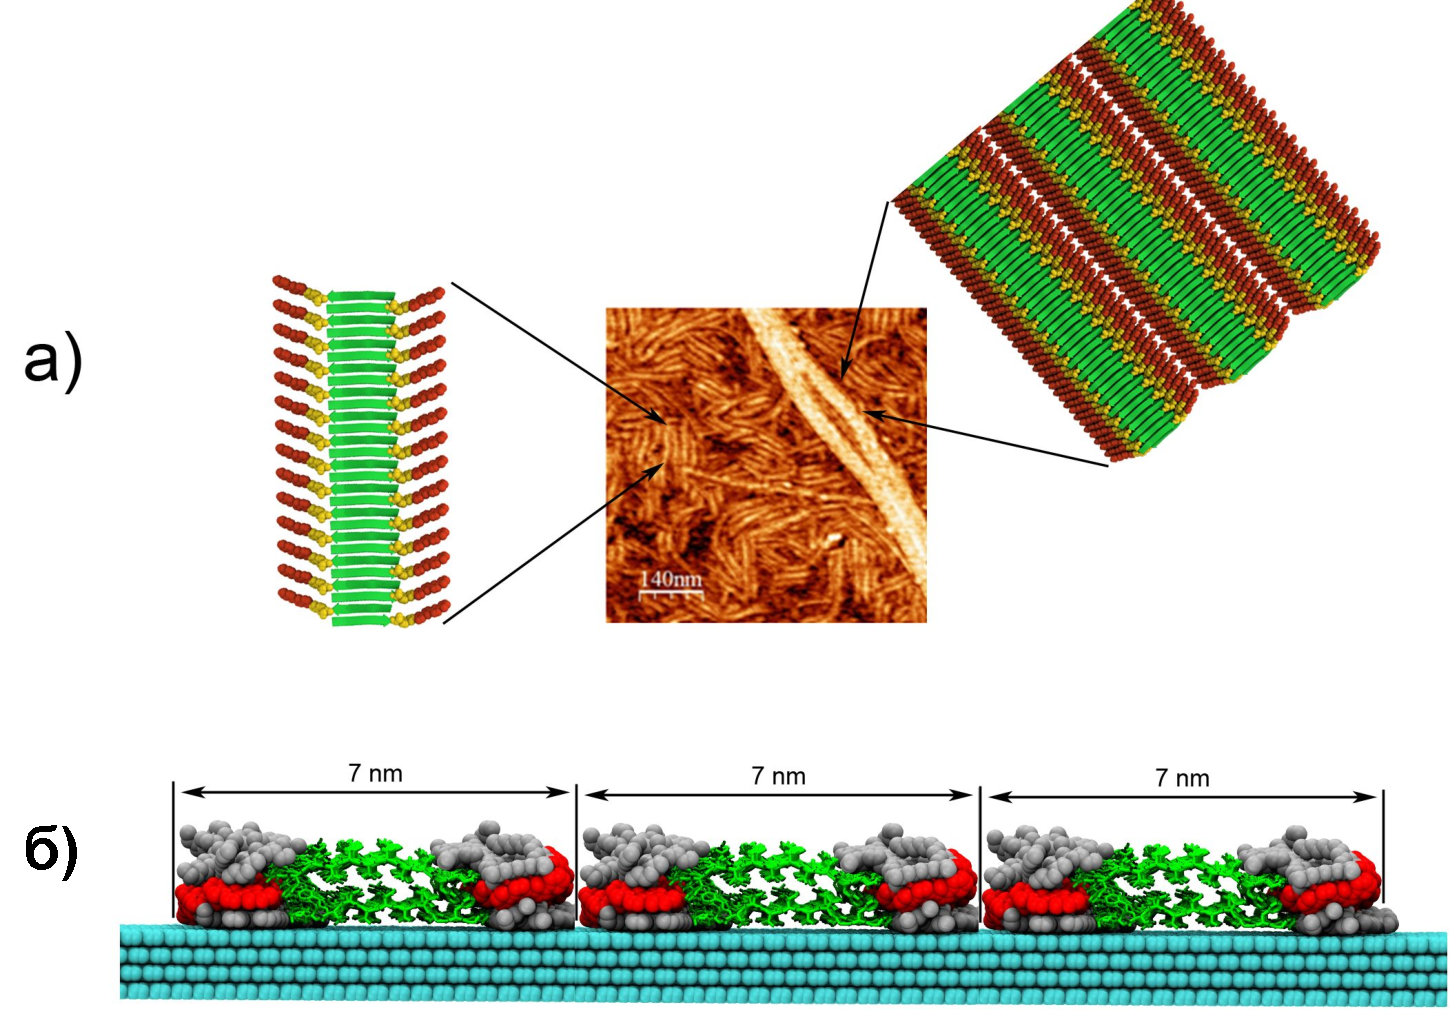
\includegraphics[width=\textwidth]{images/p4/punkt5/part4_p5_f55.pdf}
    \caption[Предложенная схематическая модель вероятного расположения гибридных молекул в наблюдаемых нанофибриллах]{Предложенная схематическая модель вероятного расположения гибридных молекул в наблюдаемых нанофибриллах и пучке, состоящем из более мелких фибрилл, образованных молекулярными гибридами тиофен-пептид. (а) Изображение АСМ и предполагаемая структура более мелких фибрилл и пучков двухслойных фибрилл. $\beta$-нити обозначены зелеными стрелками; кватротиофены изображены сферами ван-дер-Ваальса красного цвета. Алкильные цепи и ПЭГ не показаны. (б) Другой вид модели наблюдаемых пучков. Модельный субстрат изображен голубым цветом, кватротиофены - красным, алкильные цепи - серым, пептидные части - зелеными трубками, азидогруппа, связывающая тиофен с пептидом, и ПЭГ-хвосты не изображены.}
    \label{fig:p4_p5_f55}
\end{figure}
    
    
\subsubsection{Дальнейший дизайн и экспериментальные стратегии}
    
    На основании результатов моделирования и анализа экспериментальных данных можно посоветовать некоторые идеи для дальнейших экспериментальных исследований, а также возможную настройку химической структуры молекул.
    
    Дальнейшие экспериментальные исследования полученных агрегатов с помощью более совершенных методов, несомненно, будут полезны для более точного определения моделей их межмолекулярной агрегации. Могут быть применены следующие методы: (i) дифракция рентгеновских лучей на фибриллах - которая поможет определить периодичность между $\beta$-нитями и между стопками $\beta$-листов, (ii) другие методы подготовки проб АСМ (возможно, с помощью центрифугирования из более разбавленного раствора), чтобы визуализировать действительно отдельные волокна на подложке без остаточного материала, (iii) окрашивание красителем Конго красным и тиофлавином B может дать интересную информацию о структуре и кинетике самосборки фибрилл, (iv) крио-ПЭМ может быть также методом выбора для визуализации фибрилл в ``квази-растворе'', (v)  АСМ с имзмерением проводимости может пролить свет на проводящие свойства фибрилл, (vi) АСМ в растворе, если возможно, может предоставить информацию о прочности и влиянии субстрата на морфологию фибрилл.
    
    Что касается улучшения гибридных молекул тиофен-пептид в отношении потенциального использования в качестве проводящих/полупроводниковых нанопроводов, можно предложить следующие идеи. Из измерений АСМ можно увидеть, что присутствуют как более мелкие, так и большие фибриллы (пучки), это указывает на тот факт, что одна фибриллярная конформация не имеет значительных энергетических предпочтений по сравнению с другой конформацией, но разные типы агрегатов находятся в динамическом равновесии. Другой факт - полученные фибриллы кажутся не очень стабильными и не очень упорядоченными на больших расстояниях. Следовательно, можно предположить, что могут быть внесены некоторые модификации в структуру гибридных молекул, которые будут усиливать фибриллярную конформацию агрегатов и усиливать паттерны фибриллярной самосборки. Это может быть сделано, например, путем введения зарядов на двух концах $\beta$-нитей, которые будут обеспечивать самосборку из-за электростатических взаимодействий, в то же время это обеспечит антипараллельную схему самосборки. В качестве альтернативы можно исследовать различные пептидные последовательности и топологии. В том числе Schillinger et al. \cite{schillinger_oligothiophene_2009} уже было показано, что трехблочный сополимер, в котором кватротиофен присоединен к двум олигопептидам на каждом конце, образует хорошо упорядоченные фибриллы.

   Ассоциация молекул через параллельные $\beta$-листы, вероятно, будет производить более упорядоченную организацию тиофена, чем антипараллельное расположение, поэтому условия для такой сборки должны быть исследованы.

    Формирование фибриллярных агрегатов высокого порядка посредством наложения и переплетения лент также может быть перспективной стратегией, поскольку добавленное упорядочение структуры снова будет способствовать улучшению электронных и проводящих свойств.
    
\subsection{Выводы раздела}
    
    В этом разделе мы представили комплексное моделирование фибриллярных агрегатов из диблочных олигомеров кватротиофен-пептид на основе различных предполагаемых межмолекулярных структур, вдохновленных структурами родственных амилоидных фибрилл. Мы разработали мультимасштабную методологию, основанную на предсказании периодического расположения, моделировании фибрилл в явном и неявном растворителе, а также на подложке.

    Выявлены и обсуждены взаимосвязи межмолекулярной организации агрегатов, супрамолекулярной морфологии фибрилл, а также их свойств.

    Результаты моделирования сравнивались с имеющимися экспериментальными данными, и была предложена вероятная межмолекулярная структура наблюдаемых фибрилл. Были предложены дальнейшие экспериментальные и дизайнерские стратегии для создания проводящих нанопроволок из тиофен-пептидных олигомеров.
    
    
    




\section{Моделирование пептидных фибрилл EF-C, взаимодействующих с ретровирусами}
\textit{Результаты данного раздела следуют публикации \cite{yolamanova_peptide_2013}.} В данном разделе приведены результаты интегративного моделирования амилоидоподобных положительно заряженных пептидных фибрилл, которые нашли свое применения в качестве средств ускоряющих вирусную трансдукцию генетического материала в клетки. Исполльзуют методы и подходы инетгративного моделирования разработанные и описанные, в том числе, в предыдущем разделе.

\subsection{Описание экспериментальных результатов}
\textit{Описание следует публикации \cite{yolamanova_peptide_2013}.}

    
\subsubsection{Пептидные нанофибриллы EF-C ускоряют ретровирусную трансдукцию генов
и могут быть использованы для быстрой концентрации вирусов}
    
    Неэффективный перенос генов и низкие концентрации вирионов это основные ограничения ретровирусной трансдукции \cite{matrai_recent_2010}. Мы и другие ранее показали, что пептиды, полученные из человеческой спермы образуют амилоидные фибриллы, которые ускоряют доставку генов ретровирусным путем, стимулируя прикрепления вирионов к клеткам-мишеням \cite{munch_semen-derived_2007,roan_cationic_2009,kim_semen-mediated_2010,wurm_influence_2010,wurm_improved_2011,roan_peptides_2011,arnold_naturally_2012}. Однако применение этих природных фибриллообразующих пептидов ограничено умеренной эффективностью, высокой стоимостью синтез пептида и вариабельностью размера фибрилл и кинетики их образования. Здесь мы сообщаем о разработке нанофибрилл, которые самоорганизуются в водном растворе из пептида длиной в 12 аминокислотных остатков, которые называем ускоряющим фактором C (enhancing factor C, EF-C). Эти искусственные нанофибриллы значительно более эффективно усиливают процесс ретровирусного переноса генов, чем фибриллы полученные из спермы или другие усилители трансдукции. Более того, нанофибриллы EF-C позволяют концентрировать ретровирусные переносчиками путем обычного низкоскоростного центрифугирования и являются безопасными и эффективными по оценкам в исследованиях \textit{ex vivo}. Наши результаты показывают, что фибриллы EF-C представляют собой очень универсальный, удобный и широко применимый наноматериал, который имеет потенциал значительно облегчить процесс ретровирусного переноса генов в фундаментальных исследованиях и клиническом применении. 
    
    Открытие принципов, лежащих в основе конструкции нанофибрилл для ретровирусной трансдукции произошло из исследований, направленных на более точное определение взаимодействия вируса иммунодефицита человека типа 1 (ВИЧ-1) с его клеточными рецепторами. Во время этого исследования мы проанализировали влияние на вирусную инфекционность различных пептидов, полученных из гликопротеина gp120 ВИЧ-1. Мы нашли, что один пептид, EF-A (соответствует аминокислотам 413–431 gp120) приводит к увеличению инфицирования  до 34 раз (рис. \ref{fig:p4_nn2013_f1}а,б). Для определения минимальной пептидной последовательности необходимой для этого эффекта, мы исследовали варианты различной длины (от B до H) EF-A и пептид EFcon, полученный из консенсусной последовательности gp120  (рис. \ref{fig:p4_nn2013_f1}а). Обработка клеток всеми пептидами, содержащими центральную область EF-A (остатки 419–427) способствовала инфицированию ВИЧ-1 (рис. \ref{fig:p4_nn2013_f1}в), не вызывая цитотоксических эффектов. На основе этого скрининга была идентифицирована небольшая амфифильная 12-аминокислотная последовательность пептида EF-C с последовательностью QCKIKQIINMWQ (1,533 Да; pI=9,31, заряд =+2). EF-C стимулировал вирусную инфекцию с половинной максимальной активностью ($EC_{50}$) $\sim11 $мг/мл, которая примерно в четыре раза сильнее, чем у встречающихся в природе фибрилл SEVI, полученных из спермы,  (42 мг/мл; Рис. \ref{fig:p4_nn2013_f1}в,г). Предыдущие исследования показали, что образование фибрилл является необходимым условием для того, чтобы пептиды, полученные из спермы, могли способствовать ретровирусной инфекции \cite{munch_semen-derived_2007,roan_peptides_2011,arnold_naturally_2012}. Мы обнаружили, что все активные формы gp120 фрагменты (EF-A,-C,-D,-F и con) продемонстрировали амилоид-специфическое увеличение связывание Конго красного (рис. \ref{fig:p4_nn2013_f1}д) и тиофлавина T (ThT, рис. \ref{fig:p4_nn2013_f1}е) связывание. Кроме того, интенсивность флуоресценции значительно коррелировала со способностью пептидов gp120 увеличивать вирусное инфицирование. Таким образом, образование фибрилл имеет решающее значение для способности фрагментов, полученных из gp120, стимулировать ретровирусную доставку генов. Примечательно, что EF-C всегда самособирается в нанофибриллы сразу после разбавления его раствора в диметилсульфоксиде (ДМСО) в различных буферах. Это отличается от сборки фибрилл SEVI, поскольку они обычно образуются только после нескольких часов или дней перемешивания синтезированного пептида \cite{munch_semen-derived_2007,roan_cationic_2009,kim_semen-mediated_2010,wurm_improved_2011}. Нанофибриллы EF-C могут храниться не менее двух недель при комнатной температуре или $4^{\circ}C$ без потери активности по усилению трансдукции.
    
    Чтобы охарактеризовать нанофибриллы, мы проанализировали структуру и морфологию EF-C, наиболее эффективного усилителя трансдукции. С помощью атомно-силовой микроскопии (АСМ) мы обнаружили фибриллярные агрегаты диаметром 3,4$\pm$1,1 нм, длиной от $\sim$100 до 400 нм (рис. \ref{fig:p4_nn2013_f2}а, \ref{fig:p4_modeling_sf5}), а кручение с полушагам кручения в 26$\pm$2 нм (рис. \ref{fig:p4_nn2013_f2}б). Статистический анализ изображений более 50 отдельных нанофибрилл выявил, что персистентная длина находилась в диапазоне 0,5–2,9 мкм, а модуль Юнга (E) в диапазон 0,2–9,2 ГПа. Эти значения соответствуют тем, что наблюдаются для других амилоидных систем, и это означает, что фибриллы EF-C относительно жесткие по сравнению с другими биофиламентами, такими как актин (1-2 ГПа) или органические макромолекулы такие, как полимерные мицеллы ($\sim$0,4 ГПа) \cite{knowles_nanomechanics_2011,dalhaimer_single_2003}. Дальнейший биофизический анализ с использованием кругового дихроизма (КД) и инфракрасной спектроскопия с преобразованием Фурье (ИКФС) указали на присутствие преимущественно элементов вторичной структуры $\beta$-слоя и двух пиков в полосе амида-I, характерных для антипараллельного расположения $\beta$-листов \cite{cerf_antiparallel_2009} (рис. \ref{fig:p4_nn2013_f2}в). Порошковая дифракция рентгеновских лучей подтвердила типичный амилоидный паттерн дифракции с рефлексами при 4,8\AA{} и 12\AA. Для определения молекулярной структуры фибрилл EF-C экспериментально полученные структурные параметры были объединены с молекулярным моделированием \cite{shaytan_self-assembling_2011} (рис. \ref{fig:p4_nn2013_f2}г – e). Полученная модель фибрилл предполагает, что боковые цепи лизина образуют гидрофильную поверхность с высокой плотностью катионных зарядов при физиологическом pH (рис. \ref{fig:p4_nn2013_f2}е). Измерения дзета-потенциала согласуются с этим анализом и показали что фибриллы EF-C имеют чистый потенциал +17,7 $\pm$1,7 мВ, аналогично с SEVI (+17,8$\pm$1,1 мВ).
    
    Чтобы визуализировать взаимодействие фибрилл EF-C с вирионами, нанофибриллы, меченные родамином (которые усиливают вирусную инфекцию так же эффективно, как немеченые фибриллы) были смешаны с ретровирусными частицами, меченные желтым флуоресцентным белком (YFP). Поразительно, что все вирионы связались с фибриллами EF-C, за секунды. Это эффективное образование макроскопических комплексов из вирионов и фибрилл EF-C побудили нас проверить, могут ли фибриллы использоваться для осаждения и концентрирования вирионов в настольной центрифуге. Мы обнаружили, что центрифугирование ВИЧ-1 или ретровирусных векторов с фибриллами EF-C в течение 5 мин при 10 000 g осаждали практически все вирионы. Удаление супернатанта (содержащего использованную среду) с последующим ресуспендированием вирусного осадка в желаемом объеме свежей среды, позволили сконцентрировать вирионы и достиx высоких скоростей трансдукции). Примечательно, что это подход на основе нанофибрилл значительно быстрее и удобнее, чем длительное (60–90 мин) ультрацентрифугирование (50 000 g при $4^{\circ}C$), которое обычно используется для концентрирования ретровирусных частиц \cite{tiscornia_production_2006}.
    
    
\begin{figure} [H]
    \centering
    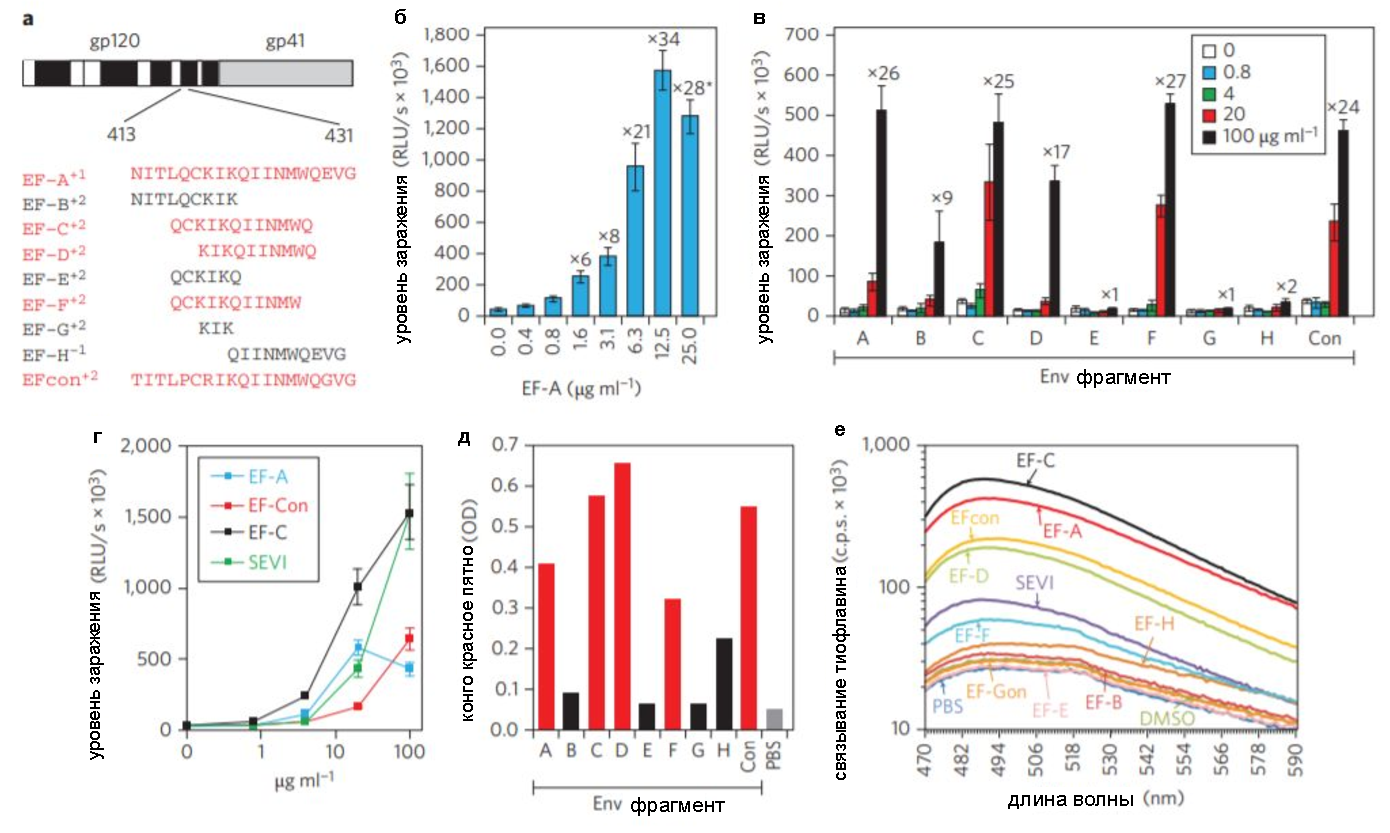
\includegraphics[width=\textwidth]{images/p4/natnanotech2013/nn2013/nn2013_f1.pdf}
    \caption[Пептиды, полученные из гликопротеина gp120 ВИЧ-1, усиливают вирусную инфекцию]{Пептиды, полученные из гликопротеина gp120 ВИЧ-1, усиливают вирусную инфекцию. \textbf{а}, Обзор проанализированных фрагментов gp120. Активные пептиды показаны красным. Указана локализация в предшественнике белке Env ВИЧ-1, а числа соответствуют положениям аминокислот в последовательности gp120 ВИЧ-1 HxB2. Цифры в верхнем индексе указывают на чистый заряд пептидов. \textbf{б}, пептид EF-A усиливает инфекцию ВИЧ-1. Вирус обрабатывали пептидом и смесь была использованы для заражения клеток TZM-bl. Цифры над столбиками указывают на n-кратное усиление инфекции по сравнению с контролем без EF-A. RLU/с, относительные световые единицы в секунду; звездочка, чрезмерное заражение. \textbf{в}, активность синтетических фрагментов gp120 по стимулированию инфицирования ВИЧ-1, описанная в \textbf{a,г}, EF-C усиливает ВИЧ-1 заражение более эффективно, чем SEVI. \textbf{д,е}, окрашивание Конго красным \textbf{д} и флуоресценция ThT \textbf{е} тестируемых пептидов. OD - оптическая плотность; c.p.s., отсчеты в секунду.}
    \label{fig:p4_nn2013_f1}
\end{figure}
    
\begin{figure} [H]
    \centering
    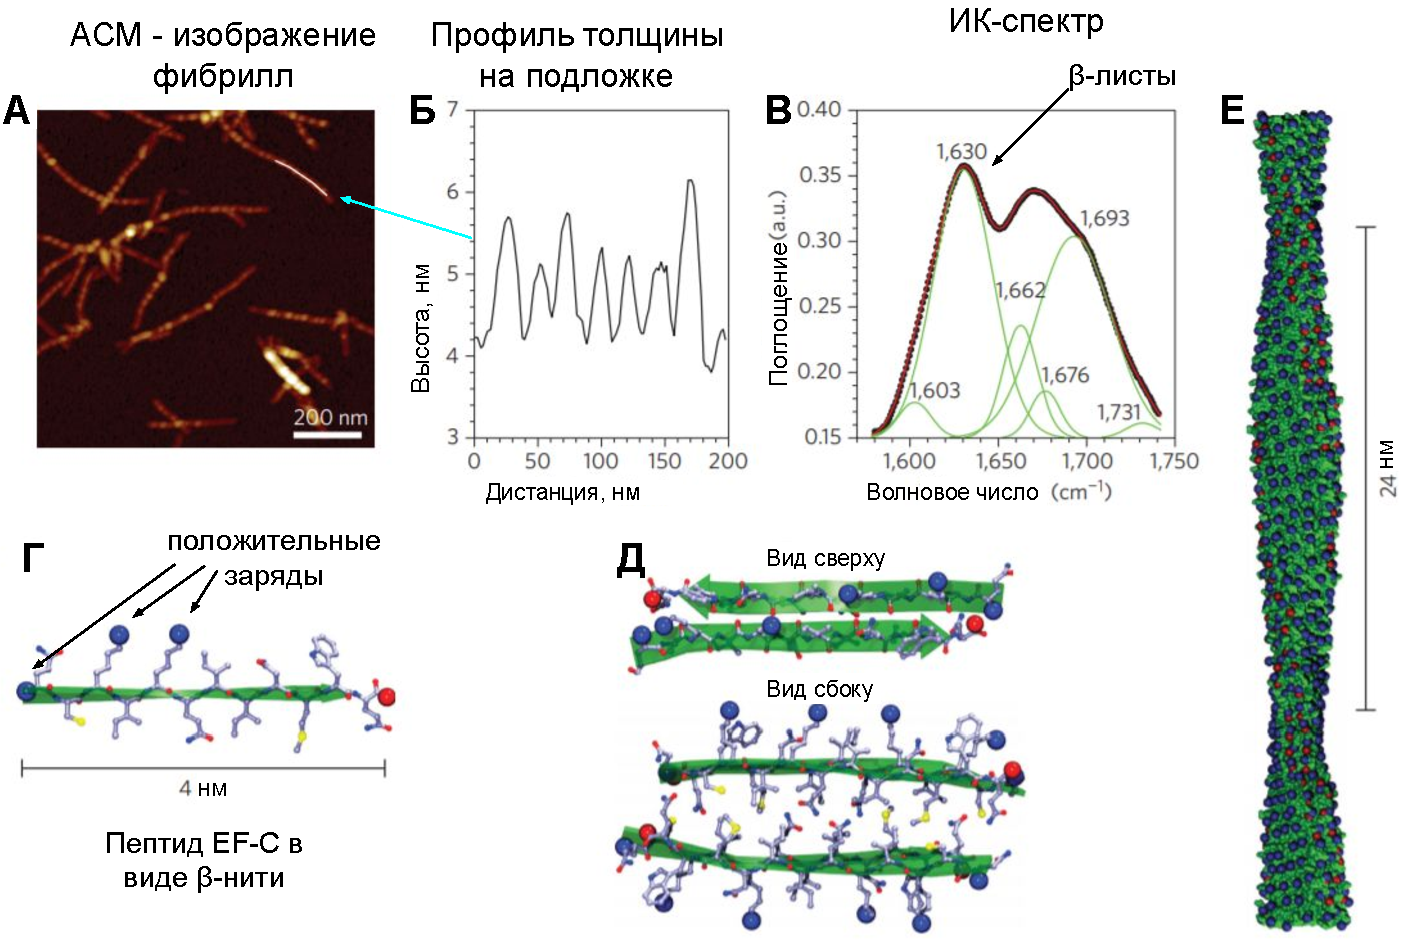
\includegraphics[width=\textwidth]{images/p4/natnanotech2013/nn2013/nn2013_f2.pdf}
    \caption[Структурная характеристика и молекулярное моделирование фибрилл EF-C]{Структурная характеристика и молекулярное моделирование фибрилл EF-C. \textbf{а} - АСМ-изображение фибрилл EF-C. \textbf{б}, профиль по указанной линии в \textbf{а}. Автокорреляция графика профиля дает средний полушаг фибрилл в 26$\pm$2 нм. \textbf{в}, ИКФС-спектр с вписыванием гауссианов для определения вторичной структуры. Пики на 1630 $см^{-1}$ и 1693 $см^{-1}$ указывают на антипараллельное расположение $\beta$-листов. \textbf{г} - Молекулярная модель пептида EF-C. \textbf{д}, вид  сверху и сбоку элементарной единицы фибриллы, состоящей из четырех $\beta$-нитей, собранных в стопку из двух антипараллельных $\beta$-листов. \textbf{е}, Уточненная молекулярная модель фибриллы с шагом спирали 28 нм. Атомы C, серый; N, синий; О, красный; S, желтый.}
    \label{fig:p4_nn2013_f2}
\end{figure}
    
    \begin{figure} [H]
    \centering
    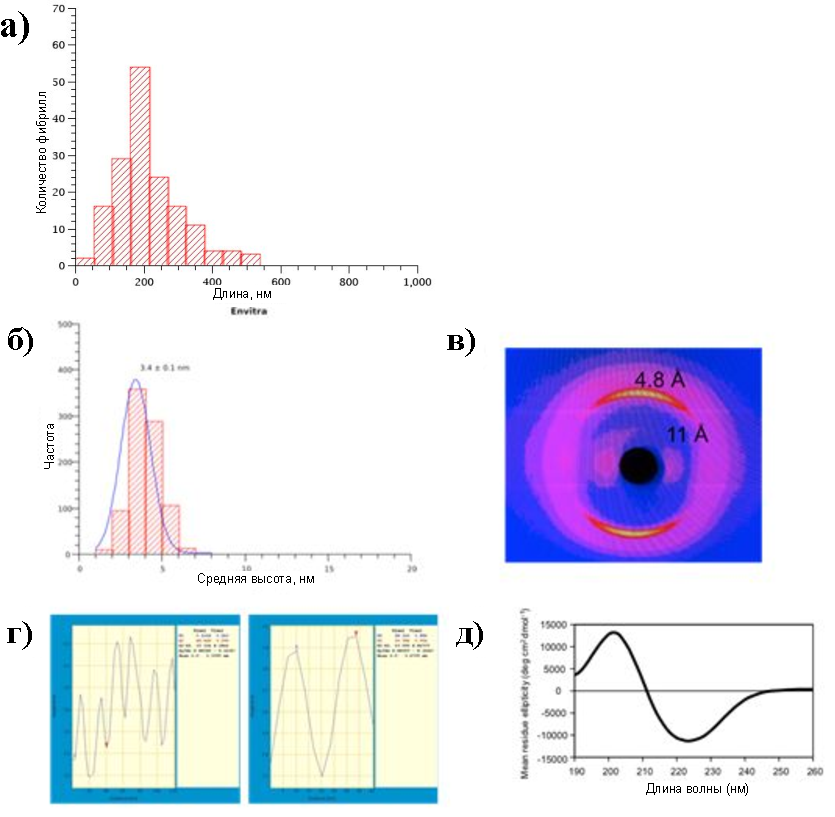
\includegraphics[width=\textwidth]{images/p4/natnanotech2013/modeling/p4_modeling_sf5.pdf}
    \caption[Дополнительная структурная характеристика фибрилл EF-C]{Дополнительная структурная характеристика фибрилл EF-C. а и б) Гистограммы распределения длин и высот АСМ . в) Рентгеновская дифрактограмма, показывающая рефлексы, характерные для амилоидных фибрилл, при 4,8 и 11\AA. г) График профиля АСМ вдоль фибриллы (слева) и соответствующая автокорреляция, показывающая половину шага спирали. д) Круговой дихроизм фибрилл EF-C в фосфатном буфере.}
    \label{fig:p4_modeling_sf5}
\end{figure}
    
% \begin{figure} [H]
%     \centering
%     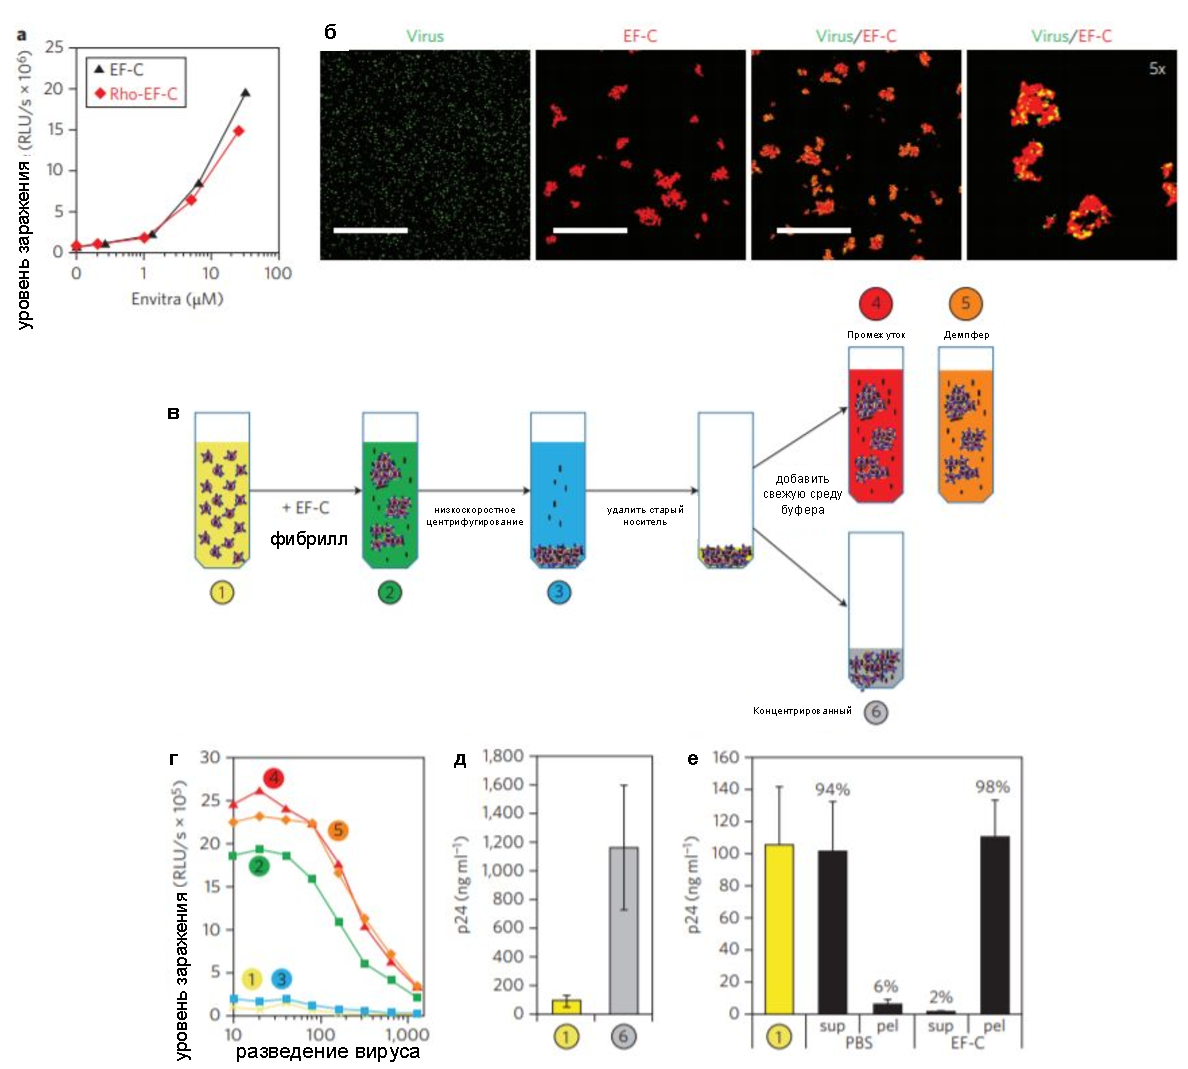
\includegraphics[width=\textwidth]{images/p4/natnanotech2013/nn2013/nn2013_f3.pdf}
%     \caption{\textbf{Фибриллы EF-C связывают, осаждают и концентрируют вирионы. а.}  Фибриллы, образованные Rho-меченным пептидом EF-C, эффективно усиливают ВИЧ-инфекцию. \textbf{б}, конфокальный микроскопические изображения (увеличение × 630) только вирионов MLV – YFP, одного Rho – EF-C или их смесей, включая увеличение последних × 5. Шкала шкалы 15 $\mu$м. \textbf{в}, Схема экспериментальной процедуры для концентрирования вирионов. 10 мл запаса вируса, содержащего использованную среду (1), составляет обработаны нанофибриллами (2) и подвергнуты низкоскоростному центрифугированию. После удаления супернатанта (3) осажденные вирионы ресуспендируют в свежем средний (4) или буферный (5). Уменьшение объема среды для ресуспендирования позволяет концентрировать вирус (6). \textbf{г}, Инфекционность полученных растворов. \textbf{д}, p24 ELISA исходного вируса (1) и вируса, обработанного нанофибриллами, после ресуспендирования в одной десятой исходного объема среды (6). \textbf{е}, p24 ELISA оригинала исходный вирус (1), супернатанты (sup), полученные после центрифугирования вируса, обработанного PBS или EF-C, и осадок (осадок), растворенный в исходном объеме.}
%     \label{fig:p4_nn2013_f3}
% \end{figure}
    

    
    Для дальнейшего выяснения механизма, лежащего в основе опосредованного фибриллами Для повышения инфекционности мы провели конфокальный микроскопический анализ комплексов вирион/фибриллы в присутствии клеток. В результаты показывают, что фибриллы EF-C значительно увеличивают количество вирусных частиц, прикрепленных к поверхности клетки. Совместная локализация с клетками указывает на стабильное взаимодействие комплексов вирион/фибриллы с клеточной мембраной. Это взаимодействие может возникнуть из нейтрализация отталкивания между отрицательно заряженными вирусными и клеточными мембранами в сочетании с привлекательными взаимодействиями избыточных положительных зарядов на фибриллах с поверхностью клетки. Это в конечном итоге приводит к усиленному слиянию вирусной и клеточной мембран.
    
    
% \begin{figure} [H]
%     \centering
%     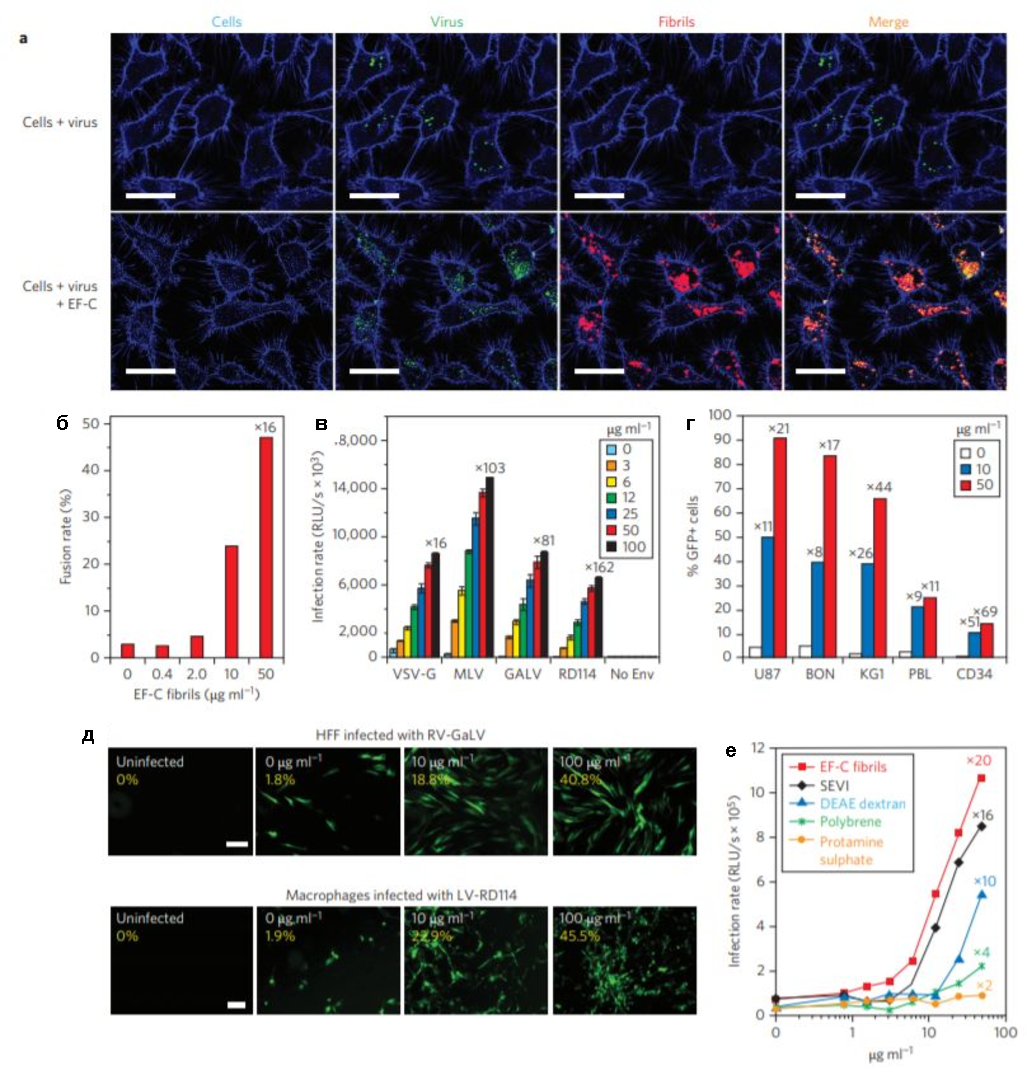
\includegraphics[width=\textwidth]{images/p4/natnanotech2013/nn2013/nn2013_f4.pdf}
%     \caption{\textbf{Фибриллы EF-C представляют собой усилители трансдукции широкого спектра действия. а,} Нанофибриллы усиливают прикрепление вирионов. Анализ клеток HeLa (синие), инокулированных либо только MLV-YFP (зеленый), либо в присутствии Rho-EF-C (красный) (увеличение × 630). Шкала шкалы 15 $\mu$м. \textbf{б}, Фибриллы увеличивают скорость слияния вирионов с клетки. \textbf{в}, фибриллы EF-C увеличивают лентивирусную трансдукцию клеток 293T независимо от вирусного гликопротеина. \textbf{г}: Влияние EF-C на перенос лентивирусного гена в глиобластома человека (U87MG), эндокринная опухоль поджелудочной железы (BON), миелоидный KG-1, мононуклеар периферической крови (PBL) и гематопоэтический ствол CD34+ клетки. \textbf{д}, Анализ фибробластов крайней плоти человека (HFF; верхняя панель) или макрофагов, происходящих из моноцитов, после трансдукции обработанными или необработанными фибриллами $\gamma$-ретровирусные (RV) или лентивирусные (LV) частицы. Указаны проценты трансдуцированных (GFP+) клеток. Шкала шкалы 50 $\mu$м. \textbf{е}, Сравнение фибрилл и других усилители трансдукции на ВИЧ-1 инфекцию. Цифры над столбиками в \textbf{в,г} и \textbf{е} указывают на n-кратное усиление трансдукции по сравнению с контролем. без фибрилл.}
%     \label{fig:p4_nn2013_f4}
% \end{figure}
    
    
    В настоящее время наиболее эффективный и распространенный метод ускорения переноса ретровирусного гена основан на производном фибронектина - RetroNectin \cite{hanenberg_colocalization_1996,hanenberg_optimization_1997,pollok_high-efficiency_1998}. RetroNectin необходимо предварительно нанести на пластины для совместной локализации вирионов и клеток, что в конечном итоге приводит к увеличению поглощения вируса клетками. Чтобы проверить, могут ли нанофибриллы работать аналогично, слайды покрывали EF-C фибриллами и инкубировали с ретровирусными частицами. Конфокальная микроскопия показала, что фибриллы были иммобилизованы на поверхности и эффективно захватывали вирионы в зависимости от времени и дозы. Как и ожидалось, иммобилизованные фибриллы значительно увеличивают лентивирусную трансдукцию и этот эффект практически не зависел от используемых пластин. Мы сравнили эффекты покрытий RetroNectin и EF-C и обнаружили, что оба усиливают ретровирусный перенос с аналогичным ускорением. Комбинация покрытия RetroNectin и фибриллами EF-C в растворе приводили к еще более высоким уровням переноса генов. Как и следовало ожидать, обработка вирионов или клеток EF-C в растворе увеличивало доставку генов ретровирусами, в то время как RetroNectin такого эффекта не имел.
    
% \begin{figure} [H]
%     \centering
%     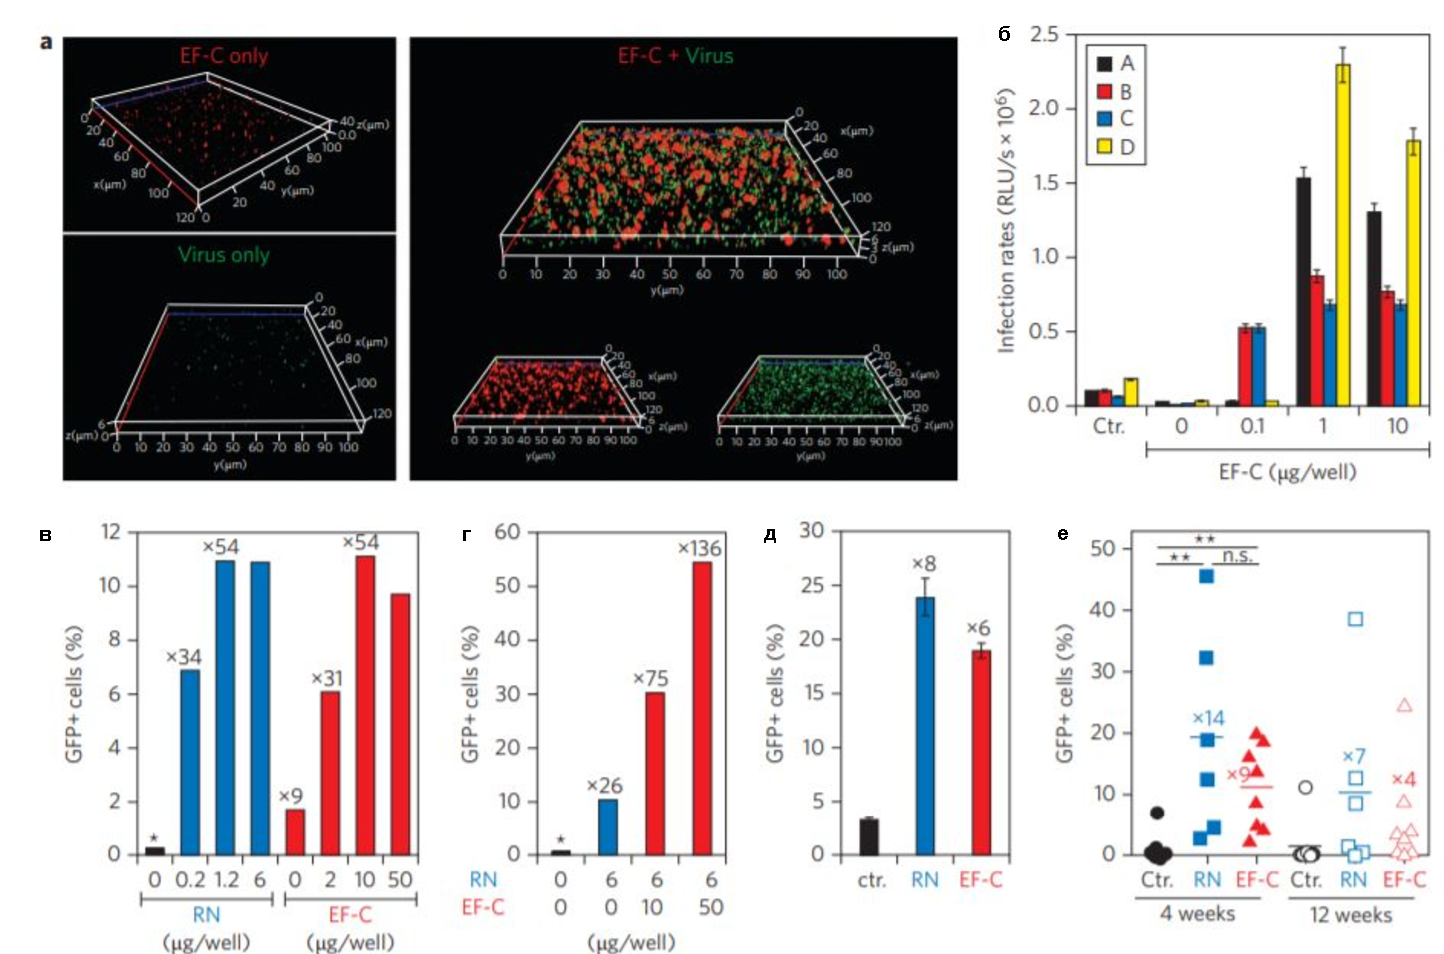
\includegraphics[width=\textwidth]{images/p4/natnanotech2013/nn2013/nn2013_f5.pdf}
%     \caption{\textbf{Фибриллы EF-C можно иммобилизовать (a – в) и обеспечить эффективный перенос генов мышам (г – е). а,} изображения Z-стека только иммобилизованных фибрилл Rho-EF-C (вверху слева), только MLV-YFP (внизу слева) и иммобилизованные фибриллы Rho-EF-C, подвергшиеся воздействию вируса (справа; на верхнем изображении показаны оба канала, слитые, и нижние изображения, отдельно). \textbf{б}, EF-C, нанесенный на микротитровальные планшеты, способствует лентивирусной инфекции. в, EF-C с покрытием усиливает лентивирусную трансдукцию с аналогичным эффективность как RetroNectin. \textbf{г}, Аддитивные эффекты ретронектина и фибрилл EF-C. Вирионы добавляли в планшеты, покрытые RetroNectin. После удаления инокулята клетки в присутствии или в отсутствие вируса, обработанного фибриллами, добавляли. \textbf{д}, фибриллы EF-C увеличивают перенос лентивирусного гена в клетки мыши. Клетки костного мозга были трансдуцированные лентивирусным вектором в отсутствие энхансера (контроль, ctr.), с использованием многоступенчатого протокола спин-инфекции (RN) на основе RetroNectin или кратким лечение EF-C. Для получения дополнительной информации см. Дополнительную информацию. \textbf{е}. Трансдуцированные клетки трансплантировали мышам-реципиентам и анализировали путем определения процент GFP-положительных клеток в периферической крови. Звездочки указывают на статистическую значимость (P<0,01). n.s .; статистически не значимо.}
%     \label{fig:p4_nn2013_f5}
% \end{figure}
    

    
    % Изучить возможное применение фибрилл EF-C в генах. подходов к терапии, мы трансдуцировали клетки костного мозга мышей \textit{ex vivo} (i) в отсутствие энхансеров, (ii) с использованием обычно используемых многоступенчатый протокол на основе ретроНектина, который включает спиновую трансдукцию \cite{millington_towards_2009,kustikova_retroviral_2007}, и (iii) в одноэтапный подход на основе нанофибрилл (для подробности см. на дополнительном рис. S16a). И РетроНектин, и EF-C нанофибриллы увеличивали трансдукцию (рис. \ref{fig:p4_nn2013_f5}д). Трансдуцированные клетки были трансплантированы мышам-реципиентам, и приживление определяли через 4–5 и 12 недель. Результаты продемонстрировали значительно более высокую долю трансдуцированных клеток в RetroNectin. и группы EF-C, чем у контрольных мышей (фиг. \ref{fig:p4_nn2013_f5}е). В частности, использование нанофибрилл EF-C вместо протокола RetroNectin уменьшилось эффективное время работы от 100 до 10 мин (доп. Рис. S16б), даже без расчета инкубации в течение ночи после покрытие и второй этап спинового заражения, необходимый для Протоколы на основе RetroNectin. Таким образом, нанофибриллы EF-C производил такие же скорости трансдукции и приживления, что и RetroNectin, но значительно сократил и упростил работу шаги (дополнительная таблица S1).
    
    % В заключение мы продемонстрировали, что пептид EF-C спонтанно самоорганизуются в высокоупорядоченные нанофибриллы, которые позволяют ускорить перенос ретровирусного гена и сконцентрировать вирионы с помощью обычного низкоскоростного центрифугирования (дополнительное Рис. S17). Положительно заряженные фибриллы эффективно захватывают вирусные частицы и увеличивают их прикрепление к клеткам-мишеням и последующее слияние. Разумное объяснение высокой эффективности трансдукции по сравнению с катионными полимерами может происходить образование электростатического ``наномоста'' между вирионами и клетками. По сравнению с катионными полимерами нанофибриллы EF-C демонстрируют отличные структурные особенности. такие как высокая жесткость и соотношение сторон. Таким образом, нанофибриллы – вирус комплексы предположительно обладают положительным суммарным зарядом, который способствует взаимодействию с отрицательной клеточной мембраной. Кроме того, некоторые вирусные гликопротеины могут оставаться доступными для взаимодействие с клеточными рецепторами для передачи инфекции. Утилизация недавно описанных нанофибрилл имеет значительные преимущества перед доступные в настоящее время методологии увеличения ретровирусной трансдукции. Во-первых, нанофибриллы EF-C более эффективны в усилении ретровирусной перенос генов по сравнению с другими макромолекулярными энхансерами. Во-вторых, Фибриллы EF-C образуются быстрее, их дешевле производить и более эффективны в усилении ретровирусной трансдукции, чем амилоидные фибриллы, полученные из спермы. В-третьих, по сравнению с РетроНектином, который был предпочтительным методом для усиления переноса ретровирусных генов более десяти лет\cite{hanenberg_colocalization_1996,hanenberg_optimization_1997,pollok_high-efficiency_1998} EF-C столь же эффективен, менее дорог и более удобен и универсален в использовании (дополнительная таблица S1). Кроме того, RetroNectin требует сложной процедуры нанесения покрытия, тогда как нанофибриллы становятся активными сразу после добавления к запас вируса или клетки-мишени. В-четвертых, нанофибриллы позволяют концентрировать вирионы в течение нескольких минут в стандартной настольной центрифуге. вместо ультрацентрифугирования. Наконец, нанофибриллы могут быть особенно подходящими для клинического применения, поскольку их универсальное обращение может обеспечить эффективный перенос ретровирусных генов в мешки для культур клеток. а также в живых организмах при местном и системном введении. Таким образом, нанофибриллы EF-C представляют собой гибкие, доступные, безопасные и новый эффективный нанобиоматериал, предлагающий большой потенциал для значительно улучшить перенос ретровирусных генов в основных и клиническое применение.
    
    
    
    
    
    
    
    
    
    
    
\subsection{Детали моделирования}

\subsection{Моделирование молекулярной динамики}

Чтобы построить молекулярную модель амилоидной фибриллы, был использован мультимасштабный комбинированный экспериментально-теоретический интегративный подход, описанный в других работах \cite{shaytan_self-assembling_2011,shaytan_self-organizing_2011}. На основе полностью атомной молекулярно-механической модели пептида EF-C, экспериментальных данных, основных физических принципов, а также понимания принципов образования амилоидных фибрилл была предложена базовая модель межмолекулярного расположения пептидов в фибрилле. Полностью атомная молекулярно-механическая модель этого межмолекулярного расположения была построена следующим образом: (i) пептид был взят в вытянутой конформации с соответствующими двугранными углами, (ii) два пептида были расположены в виде димера двух антипараллельных бета-цепей, так чтобы
максимизировать количество водородных связей между нитями, (iii) два димера были расположены в тетрамере путем наложения ``незаряженных'' поверхностей бета-листов, и тетрамер был помещен в коробку для моделирования с периодом 10\AA{} вдоль направления фибриллы, чтобы сформировать периодическую фибриллярную структуру, (iv) затем была использована модель молекулярной механики, основанная на силовом поле AMBER99SB-ILDN \cite{lindorff-larsen_improved_2010}, чтобы выполнить минимизацию энергии в фиксированных периодических граничных условиях. На следующем этапе была создана фибриллярная структура длиной 50 бета-нитей (примерно 25 нм) путем воспроизведения периодической ячейки межмолекулярного расположения в одном направлении. Фибрилла сольватирована молекулами воды (модель TIP3P), добавлено 100 ионов хлора для нейтрализации системы. Общее количество атомов в системе составило около 296 тысяч с размерами ящика периодического моделирования 11x9x30 нм. Система была подвергнута минимизации энергии с последующим моделированием релаксации с помощью МД с упругими ограничениями на положения атомов фибриллы, чтобы позволить положениям молекул ионов и воды отрелаксировать. После этого было проведено моделирование равновесной МД в течение 20 нс при давлении и температуре 1 атм и 300 К соответственно с использованием алгоритмов перемасштабирования скорости и барастата Парринелло-Рамана. Электростатические взаимодействия на больших расстояниях обрабатывались с помощью алгоритма PME, для короткодействующих взаимодействий использовалось отсечение 1 нм. Моделирование проводилось параллельно с использованием пакета программ GROMACS 4.5 \cite{van_der_spoel_gromacs_2005}. В ходе моделирования фибриллярная структура приняла свою благоприятную скрученную конформацию и была стабильной как на межмолекулярном, так и на морфологическом уровне. Структура фибриллы была дополнительно визуализирована и проанализирована с использованием VMD \cite{humphrey_vmd_1996} и собственных скриптов. Смоделированная дифракционная картина фибрилл была построена с использованием программы SFALL из пакета CCP4 \cite{winn_overview_2011} и специально написанного программного обеспечения для выполнения цилиндрического усреднения структурного фактора. Дополнительно на рис. \ref{fig:p4_modeling_sf6} представлена структура фибрилл и результаты анализа.




\begin{figure} [H]
    \centering
    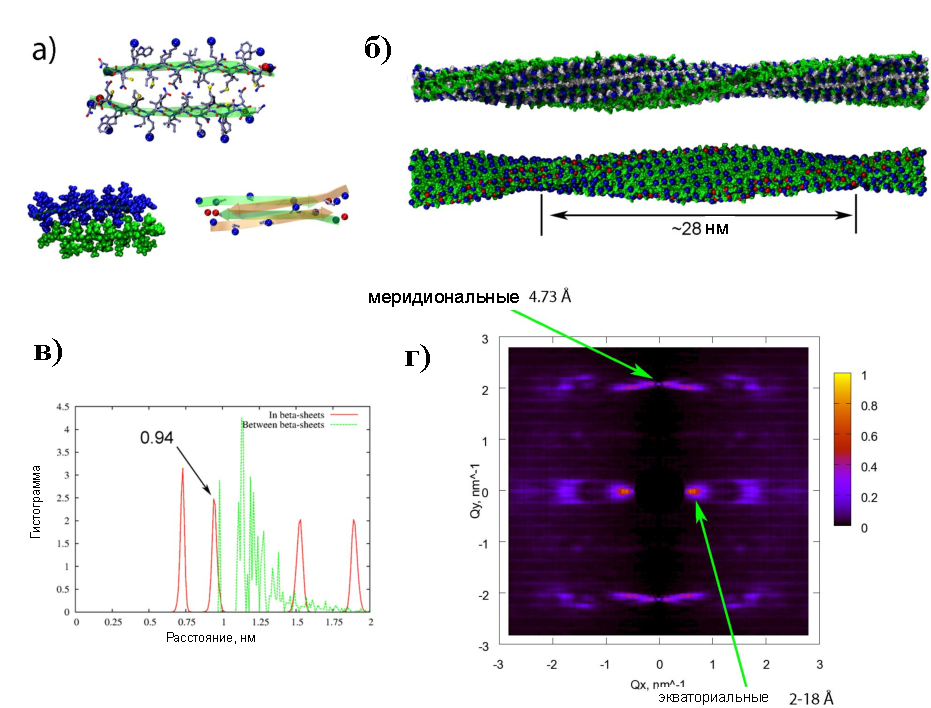
\includegraphics[width=\textwidth]{images/p4/natnanotech2013/modeling/p4_modeling_sf6.pdf}
    \caption[Дополнительные данные о модели фибриллы из пептидов EF-C]{Дополнительные данные о модели фибриллы из пептидов EF-C. а) Молекулярные модели димеров пептидов и элементарной единицы фибриллы, обрамленной четырьмя $\beta$-нитями, собранными в стопку из двух антипараллельных $\beta$-листов. б) уточненная и проанализированная модель фибриллы с использованием обширного моделирования молекулярной динамики, фибриллы представлены с использованием их доступной для растворителя поверхности: на верхнем изображении остатки окрашены в соответствии с их гидрофобностью, на нижнем - изображены положительно и отрицательно заряженные участки синим и красным, соответственно. в) распределение расстояний между центрами масс пептидов в фибрилле, видны четкие пики, показывающие одномерную периодичность фибриллы. г) рассчитанная 2D картина дифракции фибрилл, представленная как функция компонентов вектора рассеяния вдоль и перпендикулярно оси фибрилл, можно видеть четкое указание меридиональных и экваториальных рефлексов, согласующихся с экспериментальными данными (см.  рис. \ref{fig:p4_modeling_sf5}в).}
    \label{fig:p4_modeling_sf6}
\end{figure}




\section{Выводы главы \ref{part4_amyloid}}

Разработаны подходы интегративного моделирования амилоидоподобных фибрилл, позволяющие реконструировать укладку пептидов и морофологию фибрилл на основе сочетания экспериментальных данных ИК- и КД-спектроскопии, рентгеновской дифракции, электронной и атомно-силовой микроскопии.

%По результатам работы данной главы можно сделать следующие выводы:
  
 %\begin{itemize}
%\item Разработаны подходы интегративного моделирования амилоидоподобных фибрилл. Подходы основаны на: (i) использовании экспериментальных данных (рентгеновская дифракция на фибриллах, ИК- и КД-спектроскопия, окрашивание красителями) для конструирования возможных укладок пептидов в амилоидные фибриллы, (ii) использовании методов молекулярной динамики (в том числе с использованием элементов диссипативной динамики частиц) для установления крупномасштабной морфологии фибрилл с заданной укладкой, (iii) сравнении модельных морфологий с экспериментальными данными (электронная микроскопия, атомно-силовая микроскопия).
%\item В рамках комплексного теоретико-экспериментального интегративного подхода охарактеризованы структуры и морфологии фибрилл состоящих из олигомеров тиофена и пептидов (самособирающиеся биоорганические нанопровода). Получены атомистические модели фибрилл согласующиеся с экспериментальными данным. Модели фибрилл основаны на антипараллельной сборке $\beta$-листов из пептидов с последующим взаимодействием двух лент гидрофильными сторонами. Предложены стратегии улучшения проводимости самособирающихся фибрилл, основанные на использовании параллельной укладки $\beta$-листов.
%\item С помощью разработанного подхода построена структурная модель положительно заряженных фибрилл EF-C, которые могут использоваться для ускорения взаимодействия вирусных векторов с эукариотическими клетками в ходе трансдукции или генной терапии. Построенная модель согласуется с экспериментальными данными и основана на антипараллельной укладке пептидов в $\beta$-листы. Данная укладка дополнительно стабилизируется электростатическими взаимодействиями между заряженными концами пептидов.
%\end{itemize}


% \subsection{Положения выносимые на защиту}
% %положения выносимые на защиту
% \begin{enumerate}
%   \item Разработаны подходы интегративного моделирования амилоидоподобных фибрилл, позволяющие создавать их структурные атомистические модели на основе ряда косвенных экспериментальных данных. Созданы структурные модели ряда функционально перспективных фибрилл. 
% \end{enumerate}